\pdfoutput=1

%\documentclass[preprint,10pt]{elsarticle}
\documentclass[10pt]{article}
%\documentclass[review]{siamart0216}
%\documentclass{siamart0216}

%\documentclass[AMA]{WileyNJD-v1}
%\articletype{Article Type}

\usepackage{fullpage}

\usepackage{lineno}

\usepackage{amsmath,amssymb,amsfonts}
\usepackage{amsthm}
\usepackage[titletoc,toc,title]{appendix}

\usepackage{array} 
\usepackage{listings}
\usepackage{mathtools}
%\usepackage{pdfpages}
%\usepackage[textsize=footnotesize,color=green]{todonotes}
\usepackage{bm}
\usepackage{tikz}
\usepackage[normalem]{ulem}
\usepackage{hhline}

\usepackage{graphicx}
\usepackage{subfig}
\usepackage{color}

%% ====================================== graphics

\usepackage{pgfplots}
\usepackage{pgfplotstable}
\definecolor{markercolor}{RGB}{124.9, 255, 160.65}
\pgfplotsset{width=10cm,compat=1.3}
\pgfplotsset{
tick label style={font=\small},
label style={font=\small},
legend style={font=\small}
}

\usetikzlibrary{calc}

%%% START MACRO FOR ANNOTATION OF TRIANGLE WITH SLOPE %%%.
\newcommand{\logLogSlopeTriangle}[5]
{
    % #1. Relative offset in x direction.
    % #2. Width in x direction, so xA-xB.
    % #3. Relative offset in y direction.
    % #4. Slope d(y)/d(log10(x)).
    % #5. Plot options.

    \pgfplotsextra
    {
        \pgfkeysgetvalue{/pgfplots/xmin}{\xmin}
        \pgfkeysgetvalue{/pgfplots/xmax}{\xmax}
        \pgfkeysgetvalue{/pgfplots/ymin}{\ymin}
        \pgfkeysgetvalue{/pgfplots/ymax}{\ymax}

        % Calculate auxilliary quantities, in relative sense.
        \pgfmathsetmacro{\xArel}{#1}
        \pgfmathsetmacro{\yArel}{#3}
        \pgfmathsetmacro{\xBrel}{#1-#2}
        \pgfmathsetmacro{\yBrel}{\yArel}
        \pgfmathsetmacro{\xCrel}{\xArel}

        \pgfmathsetmacro{\lnxB}{\xmin*(1-(#1-#2))+\xmax*(#1-#2)} % in [xmin,xmax].
        \pgfmathsetmacro{\lnxA}{\xmin*(1-#1)+\xmax*#1} % in [xmin,xmax].
        \pgfmathsetmacro{\lnyA}{\ymin*(1-#3)+\ymax*#3} % in [ymin,ymax].
        \pgfmathsetmacro{\lnyC}{\lnyA+#4*(\lnxA-\lnxB)}
        \pgfmathsetmacro{\yCrel}{\lnyC-\ymin)/(\ymax-\ymin)} % THE IMPROVED EXPRESSION WITHOUT 'DIMENSION TOO LARGE' ERROR.

        % Define coordinates for \draw. MIND THE 'rel axis cs' as opposed to the 'axis cs'.
        \coordinate (A) at (rel axis cs:\xArel,\yArel);
        \coordinate (B) at (rel axis cs:\xBrel,\yBrel);
        \coordinate (C) at (rel axis cs:\xCrel,\yCrel);

        % Draw slope triangle.
        \draw[#5]   (A)-- node[pos=0.5,anchor=north] {1}
                    (B)-- 
                    (C)-- node[pos=0.5,anchor=west] {#4}
                    cycle;
    }
}
%%% END MACRO FOR ANNOTATION OF TRIANGLE WITH SLOPE %%%.

\newcommand{\logLogSlopeTriangleNeg}[5]
{
    % #1. Relative offset in x direction.
    % #2. Width in x direction, so xA-xB.
    % #3. Relative offset in y direction.
    % #4. Slope d(y)/d(log10(x)).
    % #5. Plot options.

    \pgfplotsextra
    {
        \pgfkeysgetvalue{/pgfplots/xmin}{\xmin}
        \pgfkeysgetvalue{/pgfplots/xmax}{\xmax}
        \pgfkeysgetvalue{/pgfplots/ymin}{\ymin}
        \pgfkeysgetvalue{/pgfplots/ymax}{\ymax}

        % Calculate auxilliary quantities, in relative sense.
        \pgfmathsetmacro{\xArel}{#1}
        \pgfmathsetmacro{\yArel}{#3}
        \pgfmathsetmacro{\xBrel}{#1-#2}
        \pgfmathsetmacro{\yBrel}{\yArel}
        \pgfmathsetmacro{\xCrel}{\xArel}

        \pgfmathsetmacro{\lnxB}{\xmin*(1-(#1-#2))+\xmax*(#1-#2)} % in [xmin,xmax].
        \pgfmathsetmacro{\lnxA}{\xmin*(1-#1)+\xmax*#1} % in [xmin,xmax].
        \pgfmathsetmacro{\lnyA}{\ymin*(1-#3)+\ymax*#3} % in [ymin,ymax].
        \pgfmathsetmacro{\lnyC}{\lnyA+#4*(\lnxA-\lnxB)}
        \pgfmathsetmacro{\yCrel}{\lnyC-\ymin)/(\ymax-\ymin)} % THE IMPROVED EXPRESSION WITHOUT 'DIMENSION TOO LARGE' ERROR.

        % Define coordinates for \draw. MIND THE 'rel axis cs' as opposed to the 'axis cs'.
        \coordinate (A) at (rel axis cs:\xArel,\yArel);
        \coordinate (B) at (rel axis cs:\xBrel,\yBrel);
        \coordinate (C) at (rel axis cs:\xCrel,\yCrel);

        % Draw slope triangle.
        \draw[#5]   (A)-- node[pos=.5,anchor=south] {1}
                    (B)-- 
                    (C)-- node[pos=0.5,anchor=west] {#4}
                    cycle;
    }
}
%%% END MACRO FOR ANNOTATION OF TRIANGLE WITH SLOPE %%%.

%%% START MACRO FOR ANNOTATION OF TRIANGLE WITH SLOPE %%%.
\newcommand{\logLogSlopeTriangleFlipNeg}[5]
{
    % #1. Relative offset in x direction.
    % #2. Width in x direction, so xA-xB.
    % #3. Relative offset in y direction.
    % #4. Slope d(y)/d(log10(x)).
    % #5. Plot options.

    \pgfplotsextra
    {
        \pgfkeysgetvalue{/pgfplots/xmin}{\xmin}
        \pgfkeysgetvalue{/pgfplots/xmax}{\xmax}
        \pgfkeysgetvalue{/pgfplots/ymin}{\ymin}
        \pgfkeysgetvalue{/pgfplots/ymax}{\ymax}

        % Calculate auxilliary quantities, in relative sense.
        %\pgfmathsetmacro{\xArel}{#1}
        %\pgfmathsetmacro{\yArel}{#3}
        \pgfmathsetmacro{\xBrel}{#1-#2}
        \pgfmathsetmacro{\yBrel}{#3}
        \pgfmathsetmacro{\xCrel}{#1}

        \pgfmathsetmacro{\lnxB}{\xmin*(1-(#1-#2))+\xmax*(#1-#2)} % in [xmin,xmax].
        \pgfmathsetmacro{\lnxA}{\xmin*(1-#1)+\xmax*#1} % in [xmin,xmax].
        \pgfmathsetmacro{\lnyA}{\ymin*(1-#3)+\ymax*#3} % in [ymin,ymax].
        \pgfmathsetmacro{\lnyC}{\lnyA+#4*(\lnxA-\lnxB)}
        \pgfmathsetmacro{\yCrel}{\lnyC-\ymin)/(\ymax-\ymin)} % THE IMPROVED EXPRESSION WITHOUT 'DIMENSION TOO LARGE' ERROR.

	\pgfmathsetmacro{\xArel}{\xBrel}
        \pgfmathsetmacro{\yArel}{\yCrel}

        % Define coordinates for \draw. MIND THE 'rel axis cs' as opposed to the 'axis cs'.
        \coordinate (A) at (rel axis cs:\xArel,\yArel);
        \coordinate (B) at (rel axis cs:\xBrel,\yBrel);
        \coordinate (C) at (rel axis cs:\xCrel,\yCrel);

        % Draw slope triangle.
        \draw[#5]   (A)-- node[pos=0.5,anchor=east] {#4}
                    (B)-- 
                    (C)-- node[pos=0.5,anchor=north] {1}
                    cycle;
    }
}
%%% END MACRO FOR ANNOTATION OF TRIANGLE WITH SLOPE %%%.


%%% START MACRO FOR ANNOTATION OF TRIANGLE WITH SLOPE %%%.
\newcommand{\logLogSlopeTriangleFlip}[5]
{
    % #1. Relative offset in x direction.
    % #2. Width in x direction, so xA-xB.
    % #3. Relative offset in y direction.
    % #4. Slope d(y)/d(log10(x)).
    % #5. Plot options.

    \pgfplotsextra
    {
        \pgfkeysgetvalue{/pgfplots/xmin}{\xmin}
        \pgfkeysgetvalue{/pgfplots/xmax}{\xmax}
        \pgfkeysgetvalue{/pgfplots/ymin}{\ymin}
        \pgfkeysgetvalue{/pgfplots/ymax}{\ymax}

        % Calculate auxilliary quantities, in relative sense.
        %\pgfmathsetmacro{\xArel}{#1}
        %\pgfmathsetmacro{\yArel}{#3}
        \pgfmathsetmacro{\xBrel}{#1-#2}
        \pgfmathsetmacro{\yBrel}{#3}
        \pgfmathsetmacro{\xCrel}{#1}

        \pgfmathsetmacro{\lnxB}{\xmin*(1-(#1-#2))+\xmax*(#1-#2)} % in [xmin,xmax].
        \pgfmathsetmacro{\lnxA}{\xmin*(1-#1)+\xmax*#1} % in [xmin,xmax].
        \pgfmathsetmacro{\lnyA}{\ymin*(1-#3)+\ymax*#3} % in [ymin,ymax].
        \pgfmathsetmacro{\lnyC}{\lnyA+#4*(\lnxA-\lnxB)}
        \pgfmathsetmacro{\yCrel}{\lnyC-\ymin)/(\ymax-\ymin)} % THE IMPROVED EXPRESSION WITHOUT 'DIMENSION TOO LARGE' ERROR.

	\pgfmathsetmacro{\xArel}{\xBrel}
        \pgfmathsetmacro{\yArel}{\yCrel}

        % Define coordinates for \draw. MIND THE 'rel axis cs' as opposed to the 'axis cs'.
        \coordinate (A) at (rel axis cs:\xArel,\yArel);
        \coordinate (B) at (rel axis cs:\xBrel,\yBrel);
        \coordinate (C) at (rel axis cs:\xCrel,\yCrel);

        % Draw slope triangle.
        \draw[#5]   (A)-- node[pos=0.5,anchor=east] {#4}
                    (B)-- 
                    (C)-- node[pos=0.5,anchor=south] {1}
                    cycle;
    }
}
%%% END MACRO FOR ANNOTATION OF TRIANGLE WITH SLOPE %%%.



\usepackage{stmaryrd}

\renewcommand{\topfraction}{0.85}
\renewcommand{\textfraction}{0.1}
\renewcommand{\floatpagefraction}{0.75}

\newcommand{\vect}[1]{\ensuremath\boldsymbol{#1}}
\newcommand{\tensor}[1]{\underline{\bm{#1}}}
\newcommand{\del}{\triangle}
\newcommand{\curl}{\grad \times}
\renewcommand{\div}{\grad \cdot}

\newcommand{\bs}[1]{\boldsymbol{#1}}
\newcommand{\equaldef}{\stackrel{\mathrm{def}}{=}}

\newcommand{\td}[2]{\frac{{\rm d}#1}{{\rm d}{\rm #2}}}
\newcommand{\pd}[2]{\frac{\partial#1}{\partial#2}}
\newcommand{\pdd}[2]{\frac{\partial^2#1}{\partial#2^2}}
\newcommand{\mb}[1]{\mathbf{#1}}
\newcommand{\mbb}[1]{\mathbb{#1}}
\newcommand{\mc}[1]{\mathcal{#1}}
\newcommand{\snor}[1]{\left| #1 \right|}
\newcommand{\nor}[1]{\left\| #1 \right\|}
\newcommand{\LRp}[1]{\left( #1 \right)}
\newcommand{\LRs}[1]{\left[ #1 \right]}
\newcommand{\LRa}[1]{\left\langle #1 \right\rangle}
\newcommand{\LRb}[1]{\left| #1 \right|}
\newcommand{\LRc}[1]{\left\{ #1 \right\}}
\newcommand{\LRceil}[1]{\left\lceil #1 \right\rceil}
\newcommand{\LRl}[1]{\left. #1 \right|}

%\newcommand{\cond}[1]{\kappa\LRp{#1}}
%\newcommand{\cond}[2]{\nor{#1}_{#2}\nor{{#1}^{-1}}_{#2}}

\newcommand{\Grad} {\ensuremath{\nabla}}
\newcommand{\Div} {\ensuremath{\nabla\cdot}}
\newcommand{\jump}[1] {\ensuremath{\llbracket#1\rrbracket}}
\newcommand{\avg}[1] {\ensuremath{\LRc{\!\{#1\}\!}}}

\newcommand{\Oh}{{\Omega_h}}
\renewcommand{\L}{L^2\LRp{\Omega}}
\newcommand{\Lk}{L^2\LRp{D^k}}
\newcommand{\Ldk}{L^2\LRp{\partial D^k}}
%\newcommand{\Lk}{D^k}
%\newcommand{\Ldk}{\partial D^k}
\newcommand{\Dhat}{\widehat{D}}
\newcommand{\Lhat}{L^2\LRp{\Dhat}}

\newtheorem{theorem}{Theorem}[section]
\newtheorem{lemma}[theorem]{Lemma}

%\newtheorem{proposition}[theorem]{Proposition}
%\newtheorem{corollary}[theorem]{Corollary}

%\newenvironment{definition}[1][Definition]{\begin{trivlist}
%\item[\hskip \labelsep {\bfseries #1}]}{\end{trivlist}}
%\newenvironment{example}[1][Example]{\begin{trivlist}
%\item[\hskip \labelsep {\bfseries #1}]}{\end{trivlist}}

\newcommand{\eval}[2][\right]{\relax
  \ifx#1\right\relax \left.\fi#2#1\rvert}

\def\etal{{\it et al.~}}


\newcommand{\note}[1]{{\color{blue}{#1}}}
%\newcommand{\remark}[1]{\textbf{\color{red}#1}}


\newcommand{\LinfDk}{L^{\infty}\LRp{D^k}}

\newcommand{\diag}[1]{{\rm diag}\LRp{#1}}

\newcommand{\half}{1/2}

\newcolumntype{C}[1]{>{\centering\let\newline\\\arraybackslash\hspace{0pt}}m{#1}}

%% d in integrand
\newcommand*\diff[1]{\mathop{}\!{\mathrm{d}#1}}

\makeatletter
\renewcommand\d[1]{\mspace{6mu}\mathrm{d}#1\@ifnextchar\d{\mspace{-3mu}}{}}
\makeatother

\date{}
\author{Jesse Chan}
\title{Weight-adjusted discontinuous Galerkin methods: matrix-valued weights and elastic wave propagation in heterogeneous media}

\begin{document}

%\title{This is the sample article title\protect\thanks{This is an example for title footnote.}}
%\author[1]{Author One*}
%\authormark{AUTHOR ONE \textsc{et al}}
%\address[1]{\orgdiv{Original Division}, \orgname{Original University}, \orgaddress{\state{State name}, \country{Country name}}}
%\corres{*Corresponding author name, This is sample corresponding address. \email{authorone@gmail.com}}


\maketitle

\linenumbers
\begin{abstract}
Weight-adjusted inner products \cite{chan2016weight1,chan2016weight2} are easily invertible approximations to weighted $L^2$ inner products.  These approximations can be paired with a discontinuous Galerkin (DG) discretization to produce a time-domain method for wave propagation which is low storage, energy stable, and high order accurate for arbitrary heterogeneous media and curvilinear meshes.  In this work, we extend weight-adjusted DG (WADG) methods to the case of matrix-valued weights, with the linear elastic wave equation as an application.  We present a DG formulation of the symmetric form of the linear elastic wave equation, with upwind-like dissipation incorporated through simple penalty fluxes.  A semi-discrete convergence analysis is given, and numerical results confirm the stability and high order accuracy of WADG for several problems in elastic wave propagation.  
\end{abstract}

%\tableofcontents

\section{Introduction}

Efficient and accurate methods for elastic wave propagation form a foundation for a broad range of applications, from seismic and medical imaging to rupture and earthquake simulation.  Finite differences are the most common choice of method \cite{virieux1986p}; however, finite element methods have garnered interest due to their low numerical dispersion and ability to accommodate geometrically flexible unstructured meshes.  

Typical methods for time-domain wave propagation utilize explicit time stepping, since the hyperbolic partial differential equations (PDEs) which govern wave propagation admit a reasonable stable time-step restriction.  However, finite element methods require the inversion of a global mass matrix when paired with explicit time integrators.  Spectral element methods (SEM) sidestep this issue on hexahedral meshes by utilizing a mass lumped diagonal mass matrix \cite{komatitsch1998spectral}.  The inversion of a globally coupled matrix can also be avoided through the use of discontinuous Galerkin (DG) methods, which result in a locally invertible block diagonal mass matrices.  Due to difficulties in extending mass-lumping techniques from hexahedra to tetrahedra, high order DG methods are often employed for seismic simulations which require the use of simplicial meshes \cite{kaser2006arbitrary, dumbser2006arbitrary, de2007arbitrary,delcourte2009high,delcourte2015analysis,ye2016discontinuous}.  High order DG methods also lend themselves well to efficient implementations using Graphics Processing Units (GPUs) \cite{klockner2009nodal, modave2015nodal, modave2016gpu, chan2015gpu}.  

Most high order DG methods on simplicial meshes assume that material coefficients are constant over each element, which can result in spurious reflections and the loss of high order accuracy \cite{castro2010seismic,mercerat2015nodal,bencomo2015discontinuous}.  This limitation can be overcome by incorporating sub-element heterogeneities into weighted mass matrices, resulting in a DG method which is both high order accurate and energy stable \cite{mercerat2015nodal, bencomo2015discontinuous}.  On tetrahedral meshes, this approach necessitates the pre-computation and storage of factorizations or inverses for each local mass matrix, which greatly increases both storage costs and data transferred at high orders of approximation.  These costs are especially problematic for accelerator architectures such as GPUs, which possess limited memory.  
%For DG methods on hexahedral meshes, mass lumping reduces the construction of weighted mass matrices to entry-wise scalings of a diagonal mass matrix.  However, on tetrahedral meshes, this approach necessitates the pre-computation and storage of factorizations for each local mass matrix, which greatly increases both storage costs and data transferred at high orders of approximation.  These costs are especially problematic for accelerator architectures such as GPUs, which possess limited memory.  

Storage costs associated with weighted mass matrices can be avoided by approximating weighted $L^2$ inner products using weight-adjusted inner products, which result in easily invertible approximations to weighted mass matrices \cite{chan2016weight1,chan2016weight2}.  For sufficiently regular weights, high order accuracy is also retained.  When paired with an energy stable DG formulation, these approximations result in weight-adjusted DG methods (WADG), which preserve energy stability and high order accuracy while retaining a low asymptotic storage cost.  Additionally, unlike mass-lumping techniques, WADG methods do not rely on the use of inexact quadrature rules, and reduce to the exact inversion of mass matrices for constant weights.  

Weight-adjusted DG methods have been applied to acoustic wave propagation in heterogeneous media and on curvilinear meshes \cite{chan2016weight1,chan2016weight2}.  Both of these previous applications have involved scalar weighting functions.  In this work, we extend weight-adjusted inner products to matrix-valued weights, and demonstrate the usefulness of this generalization to elastic wave propagation in arbitrary media.  A new energy stable DG formulation is introduced based on the symmetric form of the elastic wave equations, with upwind-like numerical dissipation introduced through simple penalty fluxes \cite{warburton2013low}.  In contrast to the fluxes proposed in \cite{ye2016discontinuous}, the penalty fluxes used here can be made to be independent of material coefficients.  

This work proceeds as follows: Sections~\ref{sec:symelas} and \ref{sec:dgform} present an energy stable DG formulation with simple penalty fluxes for the symmetric hyperbolic form of the elastic wave equation, and discuss issues related to storage and inversion of local mass matrices for material coefficients with sub-element variations.  Section~\ref{sec:mwadg} extends weight-adjusted approximations to weighted $L^2$ inner products and mass matrices to the case of matrix-valued weights, and provides interpolation estimates which account for the regularity of the matrix weight.  These results are incorporated into a weight-adjusted DG method for the linear elastic wave equations in Section~\ref{sec:wadgelas}.  Finally, numerical results in Section~\ref{sec:numerical} demonstrate the accuracy of this method for several problems in linear elasticity.  

\section{Symmetric form of the elastic wave equation}
\label{sec:symelas}
We begin with the linear elastic wave equation in a domain $\Omega \in \mathbb{R}^d$.  These equations can be written as a first order velocity-stress system for velocity $\bm{v}$ and symmetric stress tensor $\bm{S}$ 
\begin{align*}
\rho \pd{\bm{v}}{t} &= \Div{\bm{S}} + \bm{f}\\
\pd{\bm{S}}{t} &= \frac{1}{2} \tensor{\bm{C}}\LRp{\Grad\bm{v} + \Grad\bm{v}^T},
\end{align*}
where $\bm{f}$ is the body force per unit volume, $\rho$ is density, and $\tensor{\bm{C}}$ is the symmetric constitutive stiffness tensor relating stress and strain.  We rewrite these equations as a symmetric hyperbolic system of PDEs \cite{hughes1978classical} using Voigt notation
\begin{align}
\rho \pd{\bm{v}}{t} &= \sum_{i=1}^d \bm{A}_i^T \pd{\bm{\sigma}}{\bm{x}_i}\nonumber + \bm{f}\\
\bm{C}^{-1} \pd{\bm{\sigma}}{t} &= \sum_{i=1}^d \bm{A}_i \pd{\bm{v}}{\bm{x}_i}.
\label{eq:symelas}
\end{align}
where $\bm{C}$ is the symmetric matrix form of the constitutive tensor $\tensor{\bm{C}}$ and $\bm{\sigma}$ is a vector of length $N_d = \frac{d(d+1)}{2}$, the number of unique entries of the stress tensor $\bm{S}$ in $d$ dimensions.  We note that the matrices $\bm{A}_i$ are spatially constant, while $\rho,\bm{C}$, and $\bm{C}^{-1}$ can vary spatially.  Furthermore, we will assume that $\rho$ and $\bm{C}$ are positive-definite and bounded pointwise such that 
\begin{align*}
0 &< \rho_{\min} \leq \rho(\bm{x}) \leq \rho_{\max} < \infty, \\
0 &< c_{\min} \leq \bm{u}^T\bm{C}(\bm{x})\bm{u} \leq c_{\max} < \infty\\
0 &< \tilde{c}_{\min} \leq \bm{u}^T\bm{C}^{-1}(\bm{x})\bm{u} \leq \tilde{c}_{\max} < \infty
\end{align*}
for all $\bm{x}\in \mathbb{R}^d$ and all $\bm{u} \in \mathbb{R}^{N_d}$.  

In two dimensions, $\bm{v} = (\bm{v}_1, \bm{v}_2)^T$ and $\bm{\sigma}= (\sigma_{xx},\sigma_{yy},\sigma_{xy})^T$ 
\[
\bm{S} = \LRp{\begin{array}{cc}
\sigma_{xx} & \sigma_{xy}\\
\sigma_{xy} & \sigma_{yy}
\end{array}},
\]
while the matrices $\bm{A}_i$ are 
\[
\bm{A}_1 = \left(\begin{array}{cc}
1 & 0\\
0 & 0\\
0 & 1
\end{array}\right), \qquad 
\bm{A}_2 = \left(\begin{array}{cc}
0 & 0\\
0 & 1\\
1 & 0
\end{array}\right).
\]
In three dimensions, the velocity is $\bm{v} = (\bm{v}_1,\bm{v}_2,\bm{v}_3)^T$, while $\bm{\sigma}= (\sigma_{xx},\sigma_{yy},\sigma_{zz},\sigma_{yz},\sigma_{xz},\sigma_{xy})^T$ denotes the unique entries of the stress tensor $\bm{S}$
\[
\bm{S} = \LRp{\begin{array}{ccc}
\sigma_{xx} & \sigma_{xy} & \sigma_{xz}\\
\sigma_{xy} & \sigma_{yy}& \sigma_{yz}\\
\sigma_{xz} & \sigma_{yz}& \sigma_{zz}
\end{array}}.
\]
The matrices $\bm{A}_i$ are then
\[
\bm{A}_1 = \left(\begin{array}{ccc}
1 & 0 & 0\\
0 & 0& 0\\
0 & 0& 0\\
0 & 0& 0\\
0 & 0 & 1\\
0 & 1 & 0
\end{array}\right), \qquad 
\bm{A}_2 = \left(\begin{array}{ccc}
0 & 0 & 0\\
0 & 1 & 0\\
0 & 0 & 0\\
0 & 0 & 1\\
0 & 0 & 0\\
1 & 0 & 0
\end{array}\right), \qquad
\bm{A}_3 = \left(\begin{array}{ccc}
0 & 0 & 0\\
0 & 0 & 0\\
0 & 0 & 1\\
0 & 1 & 0\\
1 & 0 & 0\\
0 & 0 & 0
\end{array}\right)
\]

In general anisotropic media, $\bm{C}$ is symmetric and positive-definite.  For two-dimensional isotropic media, $\bm{C}$ is given as
\[
\bm{C}= \LRp{
\begin{array}{ccc}
2\mu+\lambda  &  \lambda  &     0\\
\lambda &       2\mu+\lambda &      0\\
0 & 0 & \mu
\end{array}}, 
\]
where $\lambda,\mu$ are Lame parameters.  For three-dimensional isotropic media, $\bm{C}$ is given instead by
\[
\LRp{\begin{array}{cccc}
2\mu+\lambda  &  \lambda  &     \lambda   & \\
\lambda &   2\mu+\lambda & \lambda   &  \\
\lambda & \lambda &   2\mu+\lambda &    \\
 &   &    & {\mu}\bm{I}^{3\times3} \\
\end{array}}.  
\]
We will consider both spatially varying isotropic and anisotropic media in this work.  

\section{An energy stable discontinuous Galerkin formulation for elastic wave propagation}
\label{sec:dgform}
The advantage of the symmetric first order formulation of the elastic wave equations (\ref{eq:symelas}) is that it is straightforward to derive an energy stable discontinuous Galerkin formulation.  We assume that the domain $\Omega$ is Lipschitz and exactly triangulated by a mesh $\Omega_h$, which consists of elements $D^k$.  We further assume that each element $D^k$ is the image of a reference element $\widehat{D}$ under the local elemental mapping 
\[
\bm{x}^k = \bm{\Phi}^k \widehat{\bm{x}},
\]
where $\bm{x}^k = \LRc{x^k,y^k}$ for $d=2$ and $\bm{x}^k = \LRc{x^k,y^k,z^k}$ for $d=3$ denote physical coordinates on $D^k$ and $\widehat{\bm{x}} = \LRc{\widehat{x},\widehat{y}}$  for $d = 2$ and $\widehat{\bm{x}} = \LRc{\widehat{x},\widehat{y},\widehat{z}}$ for $d = 3$ denote coordinates on the reference element.  We denote the determinant of the Jacobian of $\bm{\Phi}^k$ as $J$, and refer to it as the Jacobian for the remainder of this work.  

We will approximate solution components over each element $D^k$ from an approximation space $V_h\LRp{D^k}$, which we define as the composition of the mapping $\bm{\Phi}^k$ and a reference approximation space $V_h\LRp{\widehat{D}}$
\[
V_h\LRp{D^k} = \bm{\Phi}^k \circ V_h\LRp{\widehat{D}}.
\]
The global approximation space $V_h\LRp{\Oh}$ is then defined as the direct sum of elemental approximation spaces
\[
V_h\LRp{\Oh} = \bigoplus_{D^k}V_h\LRp{D^k}.  
\]
For the remainder of this work, we will take $V_h\LRp{\widehat{D}} = P^N\LRp{\widehat{D}}$, where $P^N\LRp{\widehat{D}}$ is the polynomial space of total degree $N$ on the reference simplex.  In two dimensions, $P^N$ on a triangle is
\[
P^N\LRp{\widehat{D}} = \LRc{ \widehat{x}^i \widehat{y}^j, \quad 0 \leq i + j \leq N},
\] 
and in three dimensions, $P^N$ on a tetrahedron is
\[
P^N\LRp{\widehat{D}} = \LRc{ \widehat{x}^i \widehat{y}^j \widehat{z}^k, \quad 0 \leq i + j +k \leq N}.  
\]
We denote the $L^2$ inner product and norm over $D^k$ by $\LRp{\cdot,\cdot}_{\Lk}$, such that
\[
\LRp{\bm{f},\bm{g}}_{\Lk} = \int_{D^k} \bm{f}\cdot\bm{g} \diff{\bm{x}} = \int_{\widehat{D}} \bm{f}\cdot\bm{g} J\diff{\widehat{\bm{x}}}, \qquad \nor{\bm{f}}_{\Lk}^2 = \LRp{\bm{f},\bm{f}}_{\Lk},
\]
where $\bm{f},\bm{g}$ are vector-valued functions.  Global $L^2$ inner products and norms are using local $L^2$ inner products and norms
\[
\LRp{\bm{f},\bm{g}}_{\L} = \sum_{D^k\in \Oh} \LRp{\bm{f},\bm{g}}_{\Lk}, \qquad \nor{\bm{f}}_{\L}^2 = \sum_{D^k\in \Oh} \nor{\bm{f}}^2_{\Lk}.
\]
We define also the $L^2$ inner product and norm over the boundary $\partial D^k$ of an element
\[
\LRa{\bm{u},\bm{v}}_{\Ldk} = \int_{\partial D^k}\bm{u}\cdot\bm{v}\diff{\bm{x}} = \sum_{f\in \partial D^k}\int_{\widehat{f}}\bm{u}\cdot\bm{v}J^f\diff{\widehat{\bm{x}}}, \qquad \nor{\bm{u}}_{\Ldk}^2 = \LRa{\bm{u},\bm{u}}_{\Ldk},
\]
where $J^f$ is the Jacobian of the mapping from a reference face $\widehat{f}$ to a physical face $f$ of an element.  

Let $f$ be a face of an element $D^{k}$ with neighboring element $D^{k,+}$ and unit outward normal $\bm{n}$.  We define $u^-$ and $u^+$ denote interior and exterior values of a discontinuous function $u$ such that
\[
{u}^- = \LRl{u}_{f \cap \partial D^k}, \qquad {u}^+ = \LRl{u}_{f \cap  \partial D^{k,+}}.  
\]
The jump and average of a scalar function $u\in V_h\LRp{\Omega_h}$ over $f$ are then defined as
\[
\jump{u} = u^+ - u^-, \qquad \avg{u} = \frac{u^+ + u^-}{2}.
\]
Jumps and averages of a vector-valued functions $\bm{u}\in \mathbb{R}^m$ and $\bm{S}\in \mathbb{R}^{m\times n}$ are then defined component-wise 
\[
\LRp{\jump{\bm{u}}}_i = \jump{\bm{u}_i}, \qquad 1\leq i \leq m, \qquad \LRp{\jump{\bm{S}}}_{ij} = \jump{\bm{S}_{ij}}, \qquad 1\leq i \leq m, \quad 1\leq j \leq n.
\]

We can now specify a DG formulation for the linear elastic wave equation (\ref{eq:symelas}).  Symmetric hyperbolic systems readily admit a DG formulation based on penalty fluxes \cite{chan2016short}.  For the linear elastic wave equation in symmetric first order form, this formulation is given as
\begin{align}
&\sum_{D^k\in \Oh} \LRp{\rho \pd{\bm{v}}{t},\bm{w}}_{\Lk} = \sum_{D^k\in \Oh} \LRp{\LRp{ \sum_{i=1}^d \bm{A}_i^T\pd{\bm{\sigma}}{\bm{x}_i} + \bm{f},\bm{w}}_{\Lk}  + \LRa{\frac{1}{2}\bm{A}_n^T\jump{\bm{\sigma}} + \frac{\tau_v}{2}\bm{A}_n^T\bm{A}_n\jump{\bm{v}},\bm{w}}_{\Ldk}} \nonumber\\
&\sum_{D^k\in \Oh} \LRp{\bm{C}^{-1} \pd{\bm{\sigma}}{t},\bm{q}}_{\Lk} = \sum_{D^k\in \Oh}\LRp{\LRp{\sum_{i=1}^d \bm{A}_i \pd{\bm{v}}{\bm{x}_i},\bm{q}}_{\Lk} + \LRa{\frac{1}{2}\bm{A}_n\jump{\bm{v}} + \frac{\tau_{\sigma}}{2}\bm{A}_n\bm{A}_n^T\jump{\bm{\sigma}},\bm{q}}_{\Ldk}},
\label{eq:dgform}
\end{align}
for all $\bm{w},\bm{q}\in V_h\LRp{\Omega_h}$.  Here, $\tau_v,\tau_\sigma \geq 0$ are penalty parameters and $\bm{A}_n$ is the normal matrix defined on a face $f$ as $\bm{A}_n = \sum_{i=1}^d \bm{n}_i \bm{A}_i$.  In two dimensions, $\bm{A}_n$ is 
\[
\bm{A}_n =  \LRp{\begin{array}{cc}
{n}_x & 0\\
 0 & {n}_y\\
{n}_y & {n}_x
\end{array}}.
\]
while in three dimensions, $\bm{A}_n$ is
\[
\bm{A}_n =  \LRp{\begin{array}{ccc}
{n}_x & 0 & 0\\
 0 & {n}_y & 0\\
0&  0 & {n}_z \\
0 &{n}_z & {n}_y\\
{n}_z & 0 & {n}_x\\
{n}_y & {n}_x & 0\\
\end{array}}.  
\]

We note that, unlike the penalty DG formulation given in \cite{ye2016discontinuous}, material coefficients $\rho,\bm{C}$ appear only on the left hand side of (\ref{eq:dgform}).  Thus, efficient techniques for constant coefficient formulations \cite{chan2015bbdg} can be used to evaluate the right hand side of the formulation, even in the presence of sub-element variations in $\rho,\bm{C}$.  
% and numerical fluxes are independent of these material coefficients if $\tau_v,\tau_\sigma$ are also independent of $\rho,\bm{C}$.  This implies that, even in the presence of sub-element variations in $\rho,\bm{C}$, fast constant coefficient techniques \cite{chan2015bbdg} can be used in the evaluation of the right hand side of the formulation.  

\subsection{Boundary conditions}

In this work, we assume boundary conditions on velocity and traction of the form
\[
\bm{v} = \bm{v}_{\rm bc}, \qquad \bm{S}\bm{n} = \bm{t}_{\rm bc}
\]
where $\bm{v}_{\rm bc}$ and $\bm{t}_{\rm bc}$ are given values.  Traction boundary conditions where $\bm{t}_{\rm bc} = 0$ are referred to as free-surface boundary conditions.  We follow \cite{leveque2002finite,wilcox2010high} and impose boundary conditions on the DG formulation through exterior values and jumps of the solution.  Boundary conditions on the normal component of the stress can be imposed by noting that the numerical flux contains the term $\jump{\bm{A}_n^T\bm{\sigma}} = \jump{\bm{S}\bm{n}}$.  

For a face which lies on a boundary, velocity boundary conditions are imposed by setting 
\begin{align*}
\jump{\bm{v}} &= 2\LRp{\bm{v}_{\rm bc} - \bm{v}^- }, \qquad \jump{\bm{A}_n^T\bm{\sigma}}=\jump{\bm{S}\bm{n}} = 0, 
\end{align*}
while traction boundary conditions are enforced through
\begin{align*}
\jump{\bm{A}_n^T\bm{\sigma}} = \jump{\bm{S}\bm{n}} = 2\LRp{\bm{t}_{\rm bc} - \bm{S}^-\bm{n} }= 2\LRp{\bm{t}_{\rm bc} - \bm{A}_n^T\bm{\sigma}^- }, \qquad \jump{\bm{v}} = 0.
\end{align*}
For problems which involve the truncation of infinite or large domains, absorbing boundary conditions are required.  For such cases, we impose simple non-reflective boundary conditions \cite{leveque2002finite} through jumps 
\begin{align*}
\jump{\bm{A}_n^T\bm{\sigma}} = \jump{\bm{S}\bm{n}} = - \bm{S}^-\bm{n} = -\bm{A}_n^T\bm{\sigma}^- , \qquad \jump{\bm{v}} = - \bm{v}^-. 
\end{align*}
We note that more accurate absorbing conditions can be imposed using, for example, perfectly matched layers \cite{berenger1994perfectly} or high order absorbing boundary conditions \cite{hagstrom2004new,modave2016high}.  

In all cases, boundary conditions are imposed by computing numerical fluxes using these modified jumps.  This imposition guarantees energy stability for free surface, non-reflective, and homogeneous velocity boundary conditions.  

%Easiest way to impose BCs: set $U^+$ values, compute central fluxes and then compute penalty fluxes via $\bm{A}_n^T\bm{A}_n \jump{U} = \bm{A}_n \jump{F}$.  


\subsection{Energy stability}

%It is straightforward to show that the formulation  is energy stable for zero velocity and traction boundary conditions, as well as non-reflective boundary conditions.  
Integrating the velocity equations of (\ref{eq:dgform}) by parts gives
\begin{align*}
\sum_{D^k \in \Oh}\LRp{\rho \pd{\bm{v}}{t},\bm{w}}_{\Lk} &= \sum_{D^k \in \Oh}-\LRp{ \sum_{i=1}^d \bm{\sigma},\bm{A}_i \pd{\bm{w}}{\bm{x}_i}}_{\Lk}  + \LRa{\bm{A}_n^T\avg{\bm{\sigma}} + \frac{\tau_v}{2}\bm{A}_n^T\bm{A}_n\jump{\bm{v}},\bm{w}}_{\Ldk} \nonumber\\
\sum_{D^k \in \Oh}\LRp{\bm{C}^{-1} \pd{\bm{\sigma}}{t},\bm{q}}_{\Lk} &= \sum_{D^k \in \Oh}\LRp{\sum_{i=1}^d \bm{A}_i \pd{\bm{v}}{\bm{x}_i},\bm{q}}_{\Lk} + \LRa{\frac{1}{2}\bm{A}_n\jump{\bm{v}} + \frac{\tau_{\sigma}}{2}\bm{A}_n\bm{A}_n^T\jump{\bm{\sigma}},\bm{q}}_{\Ldk} 
\end{align*}
Taking $(\bm{w},\bm{q}) = (\bm{v},\bm{\sigma})$ and adding both equations together yields
\begin{align*}
\sum_{D^k\in \Oh}&\frac{1}{2}\pd{}{t}\LRp{\LRp{\rho \bm{v},\bm{v}}_{\Lk} + \LRp{\bm{C}^{-1} \bm{\sigma},\bm{\sigma}}_{\Lk}} \\
&=\sum_{D^k\in \Omega_h}\LRa{\bm{A}_n^T\avg{\bm{\sigma}} + \frac{\tau_v}{2}\bm{A}_n^T\bm{A}_n\jump{\bm{v}},\bm{v}}_{\partial D^k}+ \LRa{\frac{1}{2}\bm{A}_n\jump{\bm{v}} + \frac{\tau_\sigma}{2}\bm{A}_n\bm{A}_n^T\jump{\bm{\sigma}},\bm{\sigma}}_{\partial D^k}  \\
&=\sum_{D^k\in \Omega_h}\sum_{f\in \partial D^k}\int_{f}\LRp{\bm{A}_n^T\avg{\bm{\sigma}}\bm{v} + \frac{\tau_v}{2}\bm{A}_n^T\bm{A}_n\jump{\bm{v}}\bm{v} + \frac{1}{2}\bm{A}_n\jump{\bm{v}}\bm{\sigma} + \frac{\tau_\sigma}{2}\bm{A}_n\bm{A}_n^T\jump{\bm{\sigma}}\bm{\sigma}}\diff{\bm{x}}.
\end{align*}
Let $\Gamma_h$ denote the set of unique faces in $\Oh$, and let $\Gamma_v,\Gamma_\sigma,\Gamma_{\rm abc}$ denote the parts of the boundary where velocity, traction, and non-reflective boundary conditions are imposed, respectively.  We separate surface terms into contributions from interior shared faces and from boundary faces.  On an interior shared face, we sum contributions from the two adjacent elements to yield
\begin{align*}
&\sum_{f\in \Gamma_h \setminus \partial \Omega} \int_{f}\LRp{\bm{A}_n^T\avg{\bm{\sigma}}\bm{v} + \frac{\tau_v}{2}\bm{A}_n^T\bm{A}_n\jump{\bm{v}}\bm{v} + \frac{1}{2}\bm{A}_n\jump{\bm{v}}\bm{\sigma} + \frac{\tau_\sigma}{2}\bm{A}_n\bm{A}_n^T\jump{\bm{\sigma}}\bm{\sigma}}\diff{\bm{x}}\\
&= - \sum_{f \in\Gamma_h \setminus \partial \Omega} \int_{f} \LRp{\frac{\tau_v}{2}\LRb{\bm{A}_n\jump{\bm{v}}}^2 + \frac{\tau_\sigma}{2}\LRb{\bm{A}_n^T\jump{\bm{\sigma}}}^2}\diff{\bm{x}}.  
%\label{thm:stability}
\end{align*}
For faces which lie on the boundary $\Gamma_v$ where velocity boundary conditions are imposed, $\jump{\bm{v}} = -2\bm{v}^-$, $\jump{\bm{A}_n^T\bm{\sigma}} = 0$, and $\bm{A}_n^T\avg{\bm{\sigma}} = \bm{Sn}^-$, implying that 
\begin{align*}
&\sum_{f\in \Gamma_v} \int_f\LRp{ \bm{A}_n^T\avg{\bm{\sigma}}\bm{v} + \frac{\tau_v}{2}\bm{A}_n^T\bm{A}_n\jump{\bm{v}}\bm{v} + \frac{1}{2}\bm{A}_n\jump{\bm{v}}\bm{\sigma} + \frac{\tau_\sigma}{2}\bm{A}_n\bm{A}_n^T\jump{\bm{\sigma}}\bm{\sigma}}\diff{\bm{x}}\\
&= \sum_{f\in \Gamma_v} \int_f \LRp{\bm{A}_n^T \bm{\sigma}^-\bm{v}^- - \bm{A}_n \bm{v}^- \bm{\sigma}^- - \tau_v \bm{A}_n^T\bm{A}_n \LRb{\bm{v}^-}^2}\diff{\bm{x}} = - \sum_{f\in \Gamma_v} \int_f \LRp{\tau_v \bm{A}_n^T\bm{A}_n \LRb{\bm{v}^-}^2}\diff{\bm{x}}.
\end{align*}
For faces which lie on $\Gamma_\sigma$, $\bm{A}_n^T\jump{\bm{\sigma}} = -2\bm{A}_n^T\bm{\sigma}^-$, $\bm{A}_n^T\avg{\bm{\sigma}} = 0$, and $\jump{\bm{v}} = 0$, yielding a similar contribution
\[
\sum_{f\in \Gamma_\sigma} \int_f \LRp{\bm{A}_n^T\avg{\bm{\sigma}}\bm{v} + \frac{\tau_v}{2}\bm{A}_n^T\bm{A}_n\jump{\bm{v}}\bm{v} + \frac{1}{2}\bm{A}_n\jump{\bm{v}}\bm{\sigma} + \frac{\tau_\sigma}{2}\bm{A}_n\bm{A}_n^T\jump{\bm{\sigma}}\bm{\sigma}}\diff{\bm{x}} = - \sum_{f\in \Gamma_\sigma} \int_f \LRp{\tau_\sigma \bm{A}_n\bm{A}_n^T \LRb{\bm{\sigma}^-}^2}\diff{\bm{x}}.
\]
Finally, for faces in $\Gamma_{\rm abc}$ we have $\bm{A}_n^T\avg{\bm{\sigma}} =\frac{1}{2} \bm{A}_n^T\bm{\sigma}^- $, $\bm{A}_n^T\jump{\bm{\sigma}} = -\bm{A}_n^T\bm{\sigma}^-$, and $\jump{\bm{v}} = -\bm{v}^-$, yielding
\begin{align*}
\sum_{f\in \Gamma_{\rm abc}} &\int_f \LRp{\bm{A}_n^T\avg{\bm{\sigma}}\bm{v} + \frac{\tau_v}{2}\bm{A}_n^T\bm{A}_n\jump{\bm{v}}\bm{v} + \frac{1}{2}\bm{A}_n\jump{\bm{v}}\bm{\sigma} + \frac{\tau_\sigma}{2}\bm{A}_n\bm{A}_n^T\jump{\bm{\sigma}}\bm{\sigma}}\diff{\bm{x}} =\\
& - \sum_{f\in \Gamma_{\rm abc}} \int_f \LRp{ \frac{\tau_v}{2} \bm{A}_n^T\bm{A}_n \LRb{\bm{v}^-}^2 + \frac{\tau_\sigma}{2} \bm{A}_n\bm{A}_n^T \LRb{\bm{\sigma}^-}^2}\diff{\bm{x}}.  
\end{align*}
Combining all face contributions together gives the following result:
\begin{theorem}
The DG formulation (\ref{eq:dgform}) is energy stable for $\tau_v,\tau_\sigma \geq 0$, in the sense that
\begin{align}
&\sum_{D^k\in \Oh} \frac{1}{2}\pd{}{t}\LRp{\LRp{\rho \bm{v},\bm{v}}_{\Lk} + \LRp{\bm{C}^{-1} \bm{\sigma},\bm{\sigma}}_{\Lk}} = - \sum_{f \in\Gamma_h \setminus \partial \Omega} \int_{f}\LRp{ \frac{\tau_v}{2}\LRb{\bm{A}_n\jump{\bm{v}}}^2 + \frac{\tau_\sigma}{2}\LRb{\bm{A}_n^T\jump{\bm{\sigma}}}^2}\diff{\bm{x}}\nonumber\\
& - \sum_{f\in \Gamma_v} \int_f \LRp{\tau_v  \LRb{\bm{A}_n\bm{v}^-}^2}\diff{\bm{x}}  - \sum_{f\in \Gamma_\sigma} \int_f \LRp{\tau_\sigma  \LRb{\bm{A}_n^T\bm{\sigma}^-}^2}\diff{\bm{x}} - \sum_{f\in \Gamma_{\rm abc}} \int_f \LRp{\frac{\tau_v}{2} \LRb{\bm{A}_n\bm{v}^-}^2 + \frac{\tau_\sigma}{2} \LRb{\bm{A}_n^T\bm{\sigma}^-}^2}\diff{\bm{x}} \leq 0.  
\label{eq:thm:stability}
\end{align}
\label{thm:stability}
\end{theorem}

Since $\rho$ and $\bm{C}^{-1}$ are positive definite, the left hand side of (\ref{eq:thm:stability}) is an $L^2$-equivalent norm on $(\bm{v},\bm{\sigma})$, and Theorem~\ref{thm:stability} implies that the magnitude of the DG solution $(\bm{v},\bm{\sigma})$ is non-increasing in time.  This also shows that dissipation present for positive penalization constants $\tau_v,\tau_{\sigma}$ acts on non-conforming components with non-zero jumps $\bm{A}_n^T\jump{\bm{v}}$ and $\bm{A}_n\jump{\bm{\sigma}}$.  In fact, it was shown in \cite{chan2016short} that, in the limit as $\tau_v,\tau_\sigma \rightarrow\infty$, the eigenspaces of DG discretizations split into a conforming part consisting of $\bm{u},\bm{\sigma}$ which satisfy
\[
\bm{A}_n\jump{\bm{u}} = 0, \qquad \bm{A}_n^T\jump{\bm{\sigma}} = 0
\]
and an non-conforming part (defined through the $L^2$ orthogonal complement) corresponding to eigenvalues contain real parts which approach $-\infty$.  For the linear elastic wave equations, these conditions are equivalent to requirements of $C^0$ continuity for $\bm{u}$ and normal continuity of the stress tensor $\jump{\bm{S}}\bm{n} = 0$.
%\begin{align*}
%\jump{\bm{S} \bm{n}} = 0.
%\jump{\bm{\sigma}_{xx} \bm{n}_x + \bm{\sigma}_{xy} \bm{n}_y + \bm{\sigma}_{xz} \bm{n}_z} &= 0\\
%\jump{\bm{\sigma}_{xy} \bm{n}_x + \bm{\sigma}_{yy} \bm{n}_y + \bm{\sigma}_{yz} \bm{n}_z} &= 0\\
%\jump{\bm{\sigma}_{xz} \bm{n}_x + \bm{\sigma}_{yz} \bm{n}_y + \bm{\sigma}_{zz} \bm{n}_z} &= 0.
%\end{align*}

\subsection{The semi-discrete matrix system for DG}

The solution to (\ref{eq:dgform}) can be approximated by discretizing in space and using an explicit time integrator, which requires only evaluations of local contributions over $D^k$ to the DG formulation
\begin{align}
\LRp{\rho \pd{\bm{v}}{t},\bm{w}}_{\Lk} &= {\LRp{ \sum_{i=1}^d \bm{A}_i^T\pd{\bm{\sigma}}{\bm{x}_i},\bm{w}}_{\Lk}  + \LRa{\frac{1}{2}\bm{A}_n^T\jump{\bm{\sigma}} + \frac{\tau_v}{2}\bm{A}_n^T\bm{A}_n\jump{\bm{v}},\bm{w}}_{\Ldk}} \nonumber\\
\LRp{\bm{C}^{-1} \pd{\bm{\sigma}}{t},\bm{q}}_{\Lk} &= {\LRp{\sum_{i=1}^d \bm{A}_i \pd{\bm{v}}{\bm{x}_i},\bm{q}}_{\Lk} + \LRa{\frac{1}{2}\bm{A}_n\jump{\bm{v}} + \frac{\tau_{\sigma}}{2}\bm{A}_n\bm{A}_n^T\jump{\bm{\sigma}},\bm{q}}_{\Ldk}}. 
\label{eq:dgloc} 
\end{align}

Let $\LRc{\phi_i}_{i=1}^{N_p}$ be a basis for $P^N\LRp{\widehat{D}}$.  We define the reference mass matrix $\widehat{\bm{M}}$ and the physical mass matrix $\bm{M}$ for an element $D^k$ as
\[
\LRp{\widehat{\bm{M}}}_{ij} = \int_{\widehat{D}}\phi_j\phi_i \diff{\widehat{\bm{x}}}, \qquad \LRp{\bm{M}}_{ij} = \int_{D^k} \phi_j\phi_i \diff{\bm{x}} = \int_{\widehat{D}}\phi_j\phi_i J\diff{ \widehat{\bm{x}}}.
\]
For affine mappings, $J$ is constant and $\bm{M} = J\widehat{\bm{M}}$.  We also define weak differentiation matrices $\bm{S}_{k}$ and face mass matrix $\bm{M}_f$ such that
\[
\LRp{\bm{S}_{k}}_{ij} =  \int_{D^k} \pd{\phi_j}{\bm{x}_k}\phi_i \diff{\bm{x}}, \qquad \LRp{\bm{M}_{f}}_{ij} =  \int_{f} \phi_j \phi_i \diff{\bm{x}} = \int_{\widehat{f}} \phi_j \phi_i J^f\diff{\widehat{\bm{x}}},
\]
where $J^f$ is the Jacobian of the mapping from a reference face $\widehat{f}$ to $f$.  For affinely mapped simplices, $J^f$ is also constant and $\bm{M}_f = J^f \widehat{\bm{M}}_f$, where the definition of the reference face mass matrix $\widehat{\bm{M}}_f$ is analogous to the definition of the reference mass matrix $\widehat{\bm{M}}$.

Finally, we define weighted mass matrices.  Let $w(\bm{x})\in \mathbb{R}$ and $\bm{W}(\bm{x})\in \mathbb{R}^{m\times n}$.  Then, scalar and matrix-weighted mass matrices $\bm{M}_w$ and $\bm{M}_{\bm{W}}$ are defined through
\[
\LRp{\bm{M}_w}_{ij} = \int_{D^k} w(\bm{x}) \phi_j(\bm{x})  \phi_i(\bm{x})\diff{\bm{x}}, \qquad \bm{M}_{\bm{W}} = \LRp{\begin{array}{ccc}
\bm{M}_{\bm{W}_{1,1}}& \ldots & \bm{M}_{\bm{W}_{1,n}}\\
\vdots & \ddots & \vdots\\
\bm{M}_{\bm{W}_{m,1}} & \ldots & \bm{M}_{\bm{W}_{m,n}}\\
\end{array}},
\]
where $\bm{M}_{\bm{W}_{i,j}}$ is the scalar weighted mass matrix weighted by the $(i,j)$ entry of $\bm{W}$. 

Local contributions to the DG variational form may then be evaluated in a quadrature-free manner using these matrices.  Let $\bm{\Sigma}_i,\bm{V}_i$ denote vectors containing degrees of freedom for solution components $\bm{\sigma}_i, \bm{v}_i$ such that 
\begin{align*}
\bm{\sigma}_{i}(\bm{x},t) &= \sum_{j=1}^{N_p} \bm{\Sigma}_i(t) \phi_j(\bm{x}), \qquad 1 \leq i \leq N_d\\ 
\bm{v}_{i}(\bm{x},t) &= \sum_{j=1}^{N_p} \bm{V}_i(t) \phi_j(\bm{x}), \qquad 1 \leq i \leq d. 
\end{align*}
Then, the local DG formulation can be written as a block system of ordinary differential equations (ODEs)
%\begin{align}
%\bm{M}_{\rho} \pd{\bm{V}_n}{t} &= \sum_{i=1}^d \sum_{j=1}^{N_d}\LRp{\bm{A}_i}_{mn} \bm{S}_{i} \bm{\Sigma}_m + \sum_{f\in \partial D^k}\bm{M}_f\bm{F}_{v,n} , \qquad n = 1,\ldots, d\nonumber\\
%\sum_{n=1}^{N_d} \bm{M}_{\bm{C}^{-1}_{mn}} \pd{\bm{\Sigma}_n}{t} &= \sum_{i=1}^d \sum_{n=1}^{d} \LRp{\bm{A}_i}_{mn}\bm{S}_{i}\bm{V}_n  +  \sum_{f\in \partial D^k}\bm{M}_f\bm{F}_{\sigma,m}, \qquad m = 1,\ldots,N_d,
%\label{eq:dgmat}
%\end{align}
%where $\bm{F}_{v,n}$ is a vector representing the $n$th component of the velocity numerical flux, $\bm{F}_{\sigma,m}$ is a vector representing the $m$th component of the stress numerical flux, and $\bm{M}_{\rho},\bm{M}_{\bm{C}^{-1}_{mn}}$ are mass matrices weighted with respect to density and the $(m,n)$ entry of $\bm{C}$, respectively.  We can rewrite this in 
by concatenating $\bm{\Sigma}_i,\bm{V}_i$ into single vectors $\bm{\Sigma},\bm{V}$ and using the Kronecker product $\otimes$
\begin{align}
\bm{M}_{\rho \bm{I}} \pd{\bm{V}}{t} &= \sum_{i=1}^d  \LRp{\bm{A}_i^T\otimes \bm{S}_{i}} \bm{\Sigma} + \sum_{f\in \partial D^k}\LRp{\bm{I}\otimes \bm{M}_f}\bm{F}_{v}\nonumber\\
\bm{M}_{\bm{C}^{-1}} \pd{\bm{\Sigma}}{t} &= \sum_{i=1}^d \LRp{\bm{A}_i\otimes \bm{S}_{i}}\bm{V}  +  \sum_{f\in \partial D^k}\LRp{\bm{I}\otimes\bm{M}_f}\bm{F}_{\sigma}. 
\label{eq:dgmat}
\end{align}
where $\bm{F}_{v}$ and $\bm{F}_{\sigma}$ denote degrees of freedom for velocity and stress numerical fluxes.  

In order to apply standard time integration methods, we must invert $\bm{M}_{\rho\bm{I}}$ and $\bm{M}_{\bm{C}^{-1}}$ to isolate $\pd{\bm{v}}{t}$ and $\pd{\bm{\sigma}}{t}$ on the left hand side.  While the inversion of $\bm{M}_{\rho\bm{I}}$ and $\bm{M}_{\bm{C}^{-1}}$ can be parallelized from element to element, doing so typically requires either the precomputation and storage of large dense matrix inverses or the on-the-fly construction and solution of a large dense matrix system at every time-step.  The former option requires a large amount of storage, while the latter option is computationally expensive and difficult to parallelize.  This cost can be overcome for $\rho, \bm{C}$ which are constant over an element $D^k$, in which case $\bm{M}_{\rho\bm{I}}$ is block diagonal with identical blocks $\bm{M}_\rho = \rho\bm{M}$, while $\bm{M}_{\bm{C}^{-1}}$ reduces to
\[
\bm{M}_{\bm{C}^{-1}} = \LRp{\begin{array}{ccc}
\bm{C}_{1,1}^{-1}\bm{M}& \ldots & \bm{C}^{-1}_{1,N_d}\bm{M}\\
\vdots & \ddots & \vdots\\
\bm{C}_{N_d,1}^{-1}\bm{M} & \ldots & \bm{C}^{-1}_{N_d,N_d}\bm{M}\\
\end{array}} 
= \LRp{\bm{C}^{-1}\otimes \bm{M}}.
\]
Then, $\bm{M}^{-1}_\rho = \frac{1}{\rho}\bm{M}^{-1} = \frac{1}{J\rho}\widehat{\bm{M}}^{-1}$, and $\bm{M}^{-1}_{\bm{C}^{-1}} = \bm{C}\otimes \bm{M}^{-1} = \bm{C}\otimes \LRp{\frac{1}{J}\widehat{\bm{M}}^{-1}}$, and each matrix inverse can be applied using the inverse of the reference mass matrix $\widehat{\bm{M}}^{-1}$ and the values of $\rho, \bm{C}$, and $J$ over each element.  Applying this observation to (\ref{eq:dgmat}) then yields the following local system of ODEs 
\begin{align*}
\pd{\bm{V}}{t} &= \sum_{i=1}^d  \LRp{\frac{1}{\rho}\bm{A}_i^T\otimes \bm{D}_{i}} \bm{\Sigma} + \sum_{f\in \partial D^k}\LRp{\frac{1}{\rho}\bm{I}\otimes \bm{L}_f}\bm{F}_{v}\\
\pd{\bm{\Sigma}}{t} &= \sum_{i=1}^d \LRp{\bm{C}\bm{A}_i\otimes \bm{D}_{i}}\bm{V}  +  \sum_{f\in \partial D^k}\LRp{\bm{C}\otimes\bm{L}_f}\bm{F}_{\sigma},
\end{align*}
where we have introduced the differentiation matrix $\bm{D}_i = \bm{M}^{-1}\bm{S}_i$ and lift matrix $\bm{L}_f = \bm{M}^{-1}\bm{M}_f$.  For affine elements, both derivative and lift matrices may be applied using only geometric factors and reference derivative and lift matrices.  

Unfortunately, if $\rho$ and $\bm{C}$ vary spatially within an element, the above approach can no longer be used to invert $\bm{M}_\rho$ and $\bm{M}_{\bm{C}^{-1}}$ in an efficient and low-storage manner.  
%One can avoid these issues by using mass lumping techniques, where nodal points for Lagrange basis functions are co-located at quadrature points on simplices \cite{chin1999higher, cohen2001higher}; however, these points are only available up to order $N\leq 4$ in three dimensions.  Additionally, these techniques can require the use of enriched polynomial spaces due to a mismatch between the number of points and dimension of $P^N$.  Mass-lumping can also be done using interior quadratures with $N_p$ points \cite{williams2014symmetric}, though these are defined only up to $N=6$ in three dimensions, and proving high order accuracy.
For isotropic media, one way to address sub-element variations in material parameters is to diagonalize the matrix $\bm{C}$ through a change of variables \cite{etienne2010hp}.  This results in a local system of ODEs with only scalar weighted mass matrices \cite{mercerat2015nodal}, which can be treated using scalar weight-adjusted approximations.  We take a different approach in addressing these issues and approximate the matrix-weighted $L^2$ inner product (and corresponding matrix-weighted mass matrix $\bm{M}_{\bm{C}^{-1}}$) using a weight-adjusted approximation which is low storage, simple to invert, energy stable, and provably high order accurate for spatially varying weights $\rho, \bm{C}$ with sufficiently regularity.   

%This implies that the RHS terms are 
%\[
%\bm{A}_1 \pd{\bm{v}}{x} + \bm{A}_2 \pd{\bm{v}}{y}  = \LRp{\begin{array}{c}
%\Div \bm{\sigma}_x \\
%\Div \bm{\sigma}_y \\
%\pd{u_1}{x} \\
%\pd{u_2}{y} \\
%\pd{u_2}{x} + \pd{u_1}{y}
%\end{array}}
%\]

%The central flux terms for elasticity are then given as
%\[
%\bm{A}_n\avg{\bm{v}} = \LRp{\begin{array}{c}
%\avg{\bm{\sigma}_x} \cdot \bm{n}\\
%\avg{\bm{\sigma}_y} \cdot \bm{n}\\
%\avg{u_1}{n}_x\\
%\avg{u_2}{n}_y\\
%\avg{u_2}{n}_x + \avg{u_1}{n}_y
%\end{array}}
%\]
%while the penalty flux term is
%\[
%\bm{A}_n^T\bm{A}_n\jump{\bm{v}} = 
%\LRp{\begin{array}{ccccc}
%1 & n_xn_y & & &\\
%n_xn_y & 1 & & &\\
% & & n_x^2 & 0 & n_xn_y \\
%  & & 0 & n_y^2 & n_xn_y \\
%   & & n_xn_y & n_xn_y & 1 
%\end{array}}
%\LRp{\begin{array}{c}
%\jump{u_1}\\
%\jump{u_2}\\
%\jump{\sigma_{xx}}\\
%\jump{\sigma_{yy}}\\
%\jump{\sigma_{xy}}
%\end{array}}
%=
%\LRp{\begin{array}{c}
%\jump{u_1} + \jump{u_2}n_xn_y\\
%n_xn_y\jump{u_1} + \jump{u_2}\\
%\LRp{\jump{\bm{\sigma}_x}\cdot\bm{n}}n_x\\
%\LRp{\jump{\bm{\sigma}_y}\cdot\bm{n}}n_y\\
%\jump{\sigma_{xy}} + n_x n_y \LRp{\jump{\sigma_{xx}} + \jump{\sigma_{yy}}}
%\end{array}}.
%\]
%We note that $\bm{A}_n^T\bm{A}_n$ has eigenvalues $1 \pm n_x n_y$ and thus has norm less than $3/2$.  
%We choose the penalty parameter $\bm{\tau}$ as a diagonal matrix such that $\bm{A}_0^{-1}\bm{\tau}\bm{A}_n^T\bm{A}_n = O(1)$.  In this case, $\tau_v = O\LRp{\frac{1}{\rho}}$, while $\tau_{\sigma} = O\LRp{\frac{1}{2\mu + \lambda}}$. 

%This implies that the RHS terms are 
%\[
%\bm{A}_1 \pd{\bm{v}}{x} + \bm{A}_2 \pd{\bm{v}}{y} +\bm{A}_3 \pd{\bm{v}}{z}  = \LRp{\begin{array}{c}
%\Div \bm{\sigma}_x \\
%\Div \bm{\sigma}_y \\
%\Div \bm{\sigma}_z \\
%\pd{u_1}{x} \\
%\pd{u_2}{y} \\
%\pd{u_3}{z} \\
%\pd{u_3}{y} + \pd{u_2}{z}\\
%\pd{u_3}{x} + \pd{u_1}{z}\\
%\pd{u_2}{x} + \pd{u_1}{y}
%\end{array}}.
%\]
%The central flux terms for elasticity are then given as
%\[
%\bm{A}_n\avg{\bm{v}} = \LRp{\begin{array}{c}
%\avg{\bm{\sigma}_x} \cdot \bm{n}\\
%\avg{\bm{\sigma}_y} \cdot \bm{n}\\
%\avg{\bm{\sigma}_z} \cdot \bm{n}\\
%\avg{u_1}{n}_x\\
%\avg{u_2}{n}_y\\
%\avg{u_3}{n}_z\\
%\avg{u_3}{n}_y + \avg{u_2}{n}_z\\
%\avg{u_3}{n}_x + \avg{u_1}{n}_z\\
%\avg{u_2}{n}_x + \avg{u_1}{n}_y
%\end{array}}
%\]
%The penalty flux term is evaluated simply by re-applying $\bm{A}_n = \bm{A}_n^T$.  Expanded out, it yields
%\begin{align*}
%\bm{A}_n^T\bm{A}_n\jump{\bm{v}} &= 
%\LRp{\begin{array}{ccc|ccc|ccc}
%1 & n_xn_y & n_xn_z   &&&&&&\\
%n_xn_y & 1 & n_yn_z   &&&&&&\\
%n_xn_z & n_yn_z & 1   &&&&&&\\
%\hline\\
%&&&  n_x^2&&&&n_xn_z&n_xn_y\\
%&&&  &n_y^2&&n_xn_z&&n_xn_y\\
%&&&  &&n_z^2&n_xn_z&n_xn_y&\\
%\hline\\
%&&&  &n_xn_z& n_xn_y& n_y^2+n_z^2&n_xn_y&n_xn_z\\
%&&&  n_xn_z && n_xn_y& n_xn_y& n_x^2+n_z^2&n_yn_z\\
%&&&  n_xn_z &n_xn_y && n_xn_z& n_yn_z& n_x^2+n_y^2\\
%\end{array}}
%\LRp{\begin{array}{c}
%\jump{u_1}\\
%\jump{u_2}\\
%\jump{u_3}\\
%\jump{\sigma_{xx}}\\
%\jump{\sigma_{yy}}\\
%\jump{\sigma_{zz}}\\
%\jump{\sigma_{yz}}\\
%\jump{\sigma_{xz}}\\
%\jump{\sigma_{xy}}
%\end{array}}\\
%&=
%\LRp{\begin{array}{c}
%\jump{u_1} + \jump{u_2}n_xn_y + \jump{u_3}n_xn_z\\
%n_xn_y\jump{u_1} + \jump{u_2} + n_yn_z\jump{u_3}\\
%n_xn_z\jump{u_1} + n_yn_z\jump{u_2} + \jump{u_3}\\
%\LRp{\jump{\bm{\sigma}_x}\cdot\bm{n}}n_x\\
%\LRp{\jump{\bm{\sigma}_y}\cdot\bm{n}}n_y\\
%\LRp{\jump{\bm{\sigma}_z}\cdot\bm{n}}n_z\\
%\jump{\sigma_{yz}}(n_y^2+n_z^2) + \LRp{\jump{\sigma_{xz}}n_y + \jump{\sigma_{xy}}n_z}n_x + \LRp{\jump{\sigma_{yy}}n_y + \jump{\sigma_{zz}}n_y}n_z\\
%\jump{\sigma_{xz}}(n_x^2+n_z^2) + \LRp{\jump{\sigma_{xx}}n_z + \jump{\sigma_{yz}}n_y}n_x + \LRp{\jump{\sigma_{xy}}n_y + \jump{\sigma_{zz}}n_x}n_z\\
%\jump{\sigma_{xy}}(n_x^2+n_y^2) + \LRp{\jump{\sigma_{xx}}n_y + \jump{\sigma_{yy}}n_y}n_x + \LRp{\jump{\sigma_{xz}}n_y + \jump{\sigma_{yz}}n_x}n_z\\
%\end{array}}.
%\end{align*}
%
%We choose the penalty parameter $\bm{\tau}$ as a diagonal matrix such that $\bm{A}_0^{-1}\bm{\tau}\bm{A}_n^T\bm{A}_n = O(1)$.  In this case, $\tau_v = O\LRp{\frac{1}{\rho}}$, while $\tau_{\sigma} = O\LRp{\frac{1}{2\mu + \lambda}}$. 

\section{Weight-adjusted inner products for matrix-valued weights}
\label{sec:mwadg}
Weight-adjusted inner products are high order accurate approximations of weighted $L^2$ inner products.  These can be interpreted as generalizations of mass lumping techniques, reducing to mass lumping when integrals are evaluated with appropriate quadrature rules.  These weight-adjusted inner products result in weight-adjusted mass matrices, whose inverses approximate the inverse of a weighted $L^2$ mass matrix.  

We wish to apply weight-adjusted approximations to avoid the inversion of $\bm{M}_\rho$ and $\bm{M}_{\bm{C}^{-1}}$.  Approximating the inverse of $\bm{M}_\rho$ can be done using weight-adjusted approximations for scalar weights \cite{chan2016weight1,chan2016weight2}, which we review in Section~\ref{sec:swadg}.  We then extend scalar weight-adjusted approximations to matrix-valued weights in Section~\ref{sec:mwadg} to approximate the inverse of $\bm{M}_{\bm{C}^{-1}}$.  

\subsection{Scalar weight adjusted inner products}
\label{sec:swadg}

We introduce standard Lebesgue $L^p$ norms and their associated $L^p$ spaces over a general domain $\Omega$
\begin{align*}
\nor{u}_{L^p\LRp{\Omega}} = \LRp{\int_{\Omega} u^p \diff{\bm{x}}}^{1/p}, \qquad  
L^p\LRp{\Omega} = \LRc{u: \Omega\rightarrow \mathbb{R}, \quad \nor{u}_{L^p\LRp{\Omega}} < \infty} 
\end{align*}
for $1 \leq p < \infty$.  For $p = \infty$, these are defined as
\begin{align*}
\nor{u}_{L^{\infty}\LRp{\Omega}} = \inf\LRc{C \geq 0: \LRb{u\LRp{\bm{x}}} \leq C \quad \forall \bm{x}\in \Omega}, \qquad L^{\infty}\LRp{\Omega} &= \LRc{u: \Omega\rightarrow \mathbb{R}, \quad \nor{u}_{L^{\infty}\LRp{\Omega}} < \infty}.
\end{align*}
These induce $L^p$ Sobolev seminorms and norms of degree $s$ 
\begin{align*}
\LRb{u}_{W^{s,p}\LRp{\Omega}} &= \LRp{\sum_{\LRb{\alpha}= s} \nor{ D^{\alpha} u}_{L^p\LRp{\Omega}}^p}^{1/p}, \qquad \LRb{u}_{W^{s,\infty}\LRp{\Omega}} = \max_{\LRb{\alpha}= s} \nor{D^{\alpha}u}_{L^{\infty}\LRp{\Omega}}\\
\nor{u}_{W^{s,p}\LRp{\Omega}} &= \LRp{\sum_{\LRb{\alpha}\leq s} \nor{ D^{\alpha} u}_{L^p\LRp{\Omega}}^p}^{1/p}, \qquad \nor{u}_{W^{s,\infty}\LRp{\Omega}} = \max_{\LRb{\alpha}\leq s} \nor{D^{\alpha}u}_{L^{\infty}\LRp{\Omega}}.
\end{align*}
where $\alpha = \LRc{\alpha_1,\ldots,\alpha_d}$ is a multi-index such that
\begin{align*}
D^{\alpha}u &= \pd{^{\alpha_1}}{x^{\alpha_1}}\pd{^{\alpha_2}}{y^{\alpha_2}} u, \qquad d = 2\\
D^{\alpha}u &= \pd{^{\alpha_1}}{x^{\alpha_1}}\pd{^{\alpha_2}}{y^{\alpha_2}}\pd{^{\alpha_3}}{z^{\alpha_3}} u, \qquad d = 3.
\end{align*}

Let $\Pi_N$ denote the $L^2$ projection on the reference element $\widehat{D}$.  We define two operators $T_w: L^2\LRp{D^k} \rightarrow P^N\LRp{D^k}$ and $T^{-1}_w: L^2\LRp{D^k} \rightarrow P^N\LRp{D^k}$ such that
\begin{align*}
T_wu &= \Pi_N(wu)\\
\LRp{wT^{-1}_wu,v}_{\Lk} &= \LRp{u,v}_{\Lk}, \qquad \forall v\in P^N\LRp{D^k}.  
\end{align*}
A weighted $L^2$ inner product $\LRp{wu,v}_{\Lk}$ can be approximated by a weight-adjusted inner product
\[
\LRp{wu,v}_{\Lk} = \LRp{T_wu,v}_{\Lk}\approx \LRp{T^{-1}_{1/w}u,v}_{\Lk}.  
\]
based on the observation that $T^{-1}_{1/w}u \approx uw$.  This approximation is made precise by the following estimates for approximations of the product $uw$ and weighted moments on affinely mapped elements:
\begin{theorem}[Theorem 5 in \cite{chan2016weight1}]
Let $D^k$ be quasi-regular with representative size $h = {\rm diam}\LRp{D^k}$.  For $N \geq 0$, $w\in W^{N+1,\infty}\LRp{D^k}$, and $u \in W^{N+1,2}\LRp{D^k}$, 
\begin{align}
\nor{{u}{w}-T_{w}u}_{L^2\LRp{D^k}} &\leq C_wh^{N+1} \nor{u}_{W^{N+1,2}\LRp{D^k}},\\
\nor{{u}{w}-T^{-1}_{1/w}u}_{L^2\LRp{D^k}} &\leq C_wh^{N+1}   \nor{u}_{W^{N+1,2}\LRp{D^k}}.
\end{align}
where $C_w = C\nor{w}_{L^{\infty}\LRp{D^k}}\nor{\frac{1}{w}}_{L^{\infty}\LRp{D^k}} \nor{w}_{W^{N+1,\infty}\LRp{D^k}}$.
\end{theorem}

%\begin{theorem}[Theorem 6 in \cite{chan2016weight1}]
%Let $u\in W^{N+1,2}\LRp{D^k}$, $w\in W^{N+1,\infty}\LRp{D^k}$, and $v \in P^M\LRp{D^k}$ for $0 \leq M\leq N$; then
%\begin{align*}
%&\LRb{\LRp{{w}u,v}_{L^2\LRp{D^k}} - \LRp{T^{-1}_{1/w}u,v}} \\
%&\leq Ch^{2N+2 - M} \nor{{w}}_{L^{\infty}\LRp{D^k}}\nor{\frac{1}{w}}_{L^{\infty}\LRp{D^k}}^2 \nor{w}^2_{W^{N+1,\infty}\LRp{D^k}}  \nor{u}_{W^{N+1,2}\LRp{D^k}} \nor{v}_{L^{\infty}\LRp{D^k}}.
%\end{align*}
%\end{theorem}
%Both theorems rely on a scalar weighted interpolation estimate derived in \cite{warburton2013low,chan2016weight1} for a general non-affine element $D^k$.  
This theorem relies on a scalar weighted interpolation estimate derived in \cite{warburton2013low,chan2016weight1} for a general non-affine element $D^k$.  
\begin{theorem}[Theorem 4 in \cite{chan2016weight1}]
Let $D^k$ be a quasi-regular element with representative size $h = {\rm diam}\LRp{D^k}$. For $N \geq 0$, $w\in W^{N+1,\infty}\LRp{D^k}$, and $u\in W^{N+1,2}\LRp{D^k}$, 
\begin{align*}
&\nor{u - \frac{1}{w}\Pi_N(wu)}_{\Lk} \leq \\
&C h^{N+1} \nor{{\sqrt{J}}}_{\LinfDk}\nor{\frac{1}{\sqrt{J}}}_{\LinfDk}\nor{\frac{1}{w}}_{\LinfDk}\nor{w}_{W^{N+1,\infty}\LRp{D^k}}\nor{u}_{W^{N+1,2}\LRp{D^k}}.
\end{align*}
\label{thm:wproj}
\end{theorem}

\subsection{Extension to matrix weights}

We now generalize weight-adjusted inner products to the case of matrix-valued weights.  We first define appropriate generalizations of norms used in Section~\ref{sec:swadg} to vector-valued functions.  Let $D^{\bm{\alpha}}\bm{v}$ denote component-wise differentiation of $\bm{v}$ with respect to a $d$-dimensional multi-index $\bm{\alpha}$.  Then, vector $L^p$ Sobolev norms for $\bm{v}(\bm{x}) \in \mathbb{R}^m$ can be defined as 
\begin{align*}
\LRb{\bm{v}}_{W^{k,p}}^p &= {\sum_{i=1}^m \LRb{\bm{v}_i}_{W^{k,p}}^p}, \qquad \nor{\bm{v}}_{W^{k,p}}^p = {\sum_{i=1}^m \nor{\bm{v}_i}_{W^{k,p}}^p} \qquad 1 \leq p < \infty,\\
\LRb{\bm{v}}_{W^{k,\infty}} &= \max_i \LRb{\bm{v}_i}_{W^{k,\infty}}, \qquad \nor{\bm{v}}_{W^{k,\infty}} = \max_i \nor{\bm{v}_i}_{W^{k,\infty}}.
\end{align*}
The corresponding Sobolev spaces $W^{k,p}$ and $W^{k,\infty}$ are defined similarly to the scalar case.  

Let $\bm{W}(\bm{x})$ be a matrix-valued weight function which is pointwise symmetric positive-definite 
\[
0 < w_{\min} \leq  \nor{\bm{W}(\bm{x})}_2 \leq w_{\max} < \infty, \qquad 0 < \tilde{w}_{\min} \leq  \nor{\bm{W}^{-1}(\bm{x})}_2 \leq \tilde{w}_{\max} < \infty, \qquad \forall \bm{x} \in \Omega.
\]
We define a $k$th order Sobolev norm for $\bm{W}(\bm{x})$ in terms of the induced $p$-norm
\begin{align*}
\nor{\bm{W}(\bm{x})}_{k,p,\infty}^p &= \sum_{\LRb{\bm{\alpha}} \leq k} \sup_{\bm{x}} \nor{D^{\bm{\alpha}}\bm{W}(\bm{x})}^p_p
\end{align*}
where $D^{\bm{\alpha}}\bm{W}(\bm{x})$ again denotes component-wise differentiation.  While this norm is not sub-multiplicative, the following bound holds
\begin{align*}
\nor{\bm{W}{\bm{v}}}_{W^{k,p}}^p &= \sum_{\LRb{\alpha}\leq k} \nor{D^{\alpha}\LRp{\bm{W}\bm{v}}}_{L^p}^p 
%\leq C_N \sum_{\LRb{\alpha}\leq k} \nor{\sum_{\LRb{\beta}\leq \alpha} \LRp{D^{\beta}\bm{W}}\LRp{D^{\alpha-\beta}\bm{v}} }_{L^p}^p\\
\leq C_N \int  \sum_{\LRb{\alpha}\leq k} \sum_{\LRb{\beta}\leq \LRb{\alpha}} \nor{\LRp{D^{\beta}\bm{W}}\LRp{D^{\alpha-\beta}\bm{v}} }_{p}^p \diff{\bm{x}}\\
&\leq C_N\int \LRp{\sum_{\LRb{\alpha}\leq k} \nor{\LRp{D^{\alpha}\bm{W}}}_p}^p \LRp{\sum_{\LRb{\alpha}\leq k} \nor{D^{\alpha}\bm{v}}_{p} }^p\diff{\bm{x}}\\
&\leq C_N \nor{\bm{W}}_{k,p,\infty}^p \nor{\bm{v}}_{k,p}^p,
\end{align*}
where we have used Leibniz's rule, Cauchy-Schwarz, and the arithmetic-geometric mean inequality.  

The following theorem extends Theorem~\ref{thm:wproj} to matrix weights by computing weighted interpolation estimates for the quantity $\bm{W}^{-1}\Pi_N\LRp{\bm{W}\bm{v}}$.  
\begin{theorem}
Let $D^k$ be a quasi-regular element with representative size $h = {\rm diam}\LRp{D^k}$. For $N \geq 0$, $\bm{W} \in \LRp{W^{N+1,\infty}\LRp{D^k}}^{d\times d}$, and $\bm{v}\in \LRp{W^{N+1,2}\LRp{D^k}}^d$, 
\[
\nor{\bm{v} - \bm{W}^{-1}\Pi_N\LRp{\bm{W}\bm{v}}}_{\Lk} \leq Ch^{N+1} \nor{{\sqrt{J}}}_{\LinfDk}\nor{\frac{1}{\sqrt{J}}}_{\LinfDk}\tilde{w}_{\max}\nor{\bm{W}}_{N+1,2,\infty} \nor{\bm{v}}_{W^{N+1,2}\LRp{D^k}}
\]
\label{thm:wwproj}
\end{theorem}
\begin{proof}
The proof is similar to the scalar case.  Using vector-valued versions of Bramble-Hilbert and a scaling argument for quasi-regular elements yields
\begin{align*}
\nor{\bm{v} - \bm{W}^{-1}\Pi_N\LRp{\bm{W}\bm{v}}}_{\Lk} &\leq C_1 \nor{\sqrt{J}}_{\LinfDk} \sup_{\bm{x}}\nor{\bm{W}^{-1}}_{2} \nor{\bm{W}\bm{v} - \Pi_N\LRp{\bm{W}\bm{v}}}_{\Lk}\\
&\leq C_1 \nor{{\sqrt{J}}}_{\LinfDk} \sup_{\bm{x}}\nor{\bm{W}^{-1}}_{2} \LRb{\bm{W}\bm{v}}_{W^{N+1,2}\LRp{\Dhat}}\\
&\leq C_2 h^{N+1}\nor{{\sqrt{J}}}_{\LinfDk}\nor{\frac{1}{\sqrt{J}}}_{\LinfDk} \sup_{\bm{x}}\nor{\bm{W}^{-1}}_{2} \nor{\bm{W}\bm{v}}_{W^{N+1,2}\LRp{D^k}}\\
&\leq C_3 h^{N+1}\nor{{\sqrt{J}}}_{\LinfDk}\nor{\frac{1}{\sqrt{J}}}_{\LinfDk} \tilde{w}_{\max} \nor{\bm{W}}_{{N+1,2,\infty}}\nor{\bm{v}}_{W^{N+1,2}\LRp{D^k}}.
\end{align*}
\end{proof}

\subsubsection{Weight-adjusted approximations with matrix weights}
\label{sec:mwadgprop}

Let $\Pi_N\bm{u}$ be defined as the $L^2$ projection applied to each component of the vector-valued function $\bm{u}$.  We then define the operator $T_{\bm{W}}$ analogously to the scalar case
\[
T_{\bm{W}}\bm{v} = \Pi_N\LRp{\bm{W}\bm{v}}.  
\]
The inverse operator $T^{-1}_{\bm{W}}$ is defined implicitly via
\[
\LRp{\bm{W}T^{-1}_{\bm{W}}\bm{v},\bm{w}}_{\Lk} = \LRp{\bm{v},\bm{w}}_{\Lk}.
\]
This definition is a straightforward generalization of $T^{-1}_{w}$ to matrix-valued weights $\bm{W}$.  Conveniently, all properties of $T_{w},T^{-1}_{w}$ for scalar $w(\bm{x})$ \cite{chan2016weight1} carry over to matrix weights $\bm{W}(\bm{x})$ as well.
\begin{lemma}
Let $\Pi_N$ denote the component-wise $L^2$ projection, and let $\bm{W} \in \LRp{L^{\infty}}^m$.  Then, $T_{\bm{W}}$ satisfies the following properties:
\begin{enumerate}
\vspace{.5em}
\item $T_{\bm{W}}^{-1}T_{\bm{W}} = \Pi_N$ \label{p1}
\vspace{.5em}
\item $\Pi_N T_{\bm{W}}^{-1} = T_{\bm{W}}^{-1}\Pi_N  =  T_{\bm{W}}^{-1}$ \label{p2}
\vspace{.5em}
\item $\nor{T^{-1}_{\bm{W}}}_{\Lk} \leq \tilde{w}_{\max}$. \label{p4}
\vspace{.5em}
\item $\LRp{T^{-1}_{\bm{W}} \bm{v},\bm{w}}_{\Lk}$ forms an inner product on $\LRp{P^N}^m \times \LRp{P^N}^m$, which is equivalent to the $L^2$ inner product with equivalence constants $C_1 = \tilde{w}_{\min}, C_2 = \tilde{w}_{\max}$. \label{p3}
\vspace{.5em}
\end{enumerate}
\label{lemma:props}
\end{lemma}
\begin{proof}
The proofs of properties~\ref{p1} and \ref{p2} are consequences of the definition of $T_{\bm{W}}$, and are identical to proofs for the scalar case.  Property~\ref{p4} is a straightforward extension from the scalar case.  Let $\bm{v}\in \LRp{P^N}^m$.  Then, 
\[
\LRp{T^{-1}_{\bm{W}} \bm{v},\bm{v}}_{\Lk} = \LRp{\bm{W}^{-1}\bm{W}T^{-1}_{\bm{W}} \bm{v},\bm{v}}_{\Lk} \leq \sup_{\bm{x}}\nor{\bm{W}^{-1}(\bm{x})}\LRp{\bm{W}T^{-1}_{\bm{W}} \bm{v},\bm{v}}_{\Lk} = \tilde{w}_{\max} \nor{\bm{v}}_{\Lk}^2.
\]
Property~\ref{p3} then simply requires the lower bound
\[
\LRp{T^{-1}_{\bm{W}} \bm{v},\bm{v}}_{\Lk} = \LRp{\bm{W}^{-1}\bm{W}T^{-1}_{\bm{W}} \bm{v},\bm{v}}_{\Lk} \geq \inf_{\bm{x}}\nor{\bm{W}^{-1}(\bm{x})}\nor{\bm{v}}_{\Lk}^2 = \tilde{w}_{\min}\nor{\bm{v}}_{\Lk}^2 .  
\]
\end{proof}

Using Theorem~\ref{thm:wwproj}, we may also show that the matrix-valued weight-adjusted inner product is also high order accurate for sufficiently regular $\bm{W}$.
\begin{theorem}
Let $D^k$ be a quasi-regular element with representative size $h = {\rm diam}\LRp{D^k}$. For $N > 0$
\[
\nor{ \bm{W}\bm{v} - {T}^{-1}_{\bm{W}^{-1}}\bm{v} }_{\Lk } \leq C_{\bm{W}} h^{N+1} \nor{\bm{v}}_{W^{N+1,2}\LRp{D^k}}
\]
with constant $C_{\bm{W}}$ depending on $\bm{W}$ and $N$
\[
%C_{\bm{W}} = C_N \cond{\bm{W}}{2,\infty} \nor{\bm{W}}_{W^{N+1,2}\LRp{D^k}}.  
C_{\bm{W}} = C_N \nor{\sqrt{J}}_{\LinfDk}\nor{\frac{1}{\sqrt{J}}}_{\LinfDk} \tilde{w}_{\max}{w}_{\max} \nor{\bm{W}}_{{N+1,2,\infty}}.  
\]
\label{thm:west}
\end{theorem}
\begin{proof}
The proof follows the scalar case.  The triangle inequality gives
\[
\nor{ \bm{W}\bm{v} - {T}^{-1}_{\bm{W}^{-1}}\bm{v} }_{\Lk } \leq \nor{ \bm{W}\bm{v} - \Pi_N(\bm{W}\bm{v})}_{\Lk} + \nor{\Pi_N(\bm{W}\bm{v}) - T^{-1}_{\bm{W}^{-1}}\bm{v} }_{\Lk }.  
\]
The former term is bounded by interpolation estimates and by arguments used in the proof of Theorem~\ref{thm:wwproj}.  The latter term is bounded 
\begin{align*}
\nor{\Pi_N(\bm{W}\bm{v})- T^{-1}_{\bm{W}^{-1}}\bm{v} }_{\Lk} &= \nor{T^{-1}_{\bm{W}^{-1}} T_{\bm{W}^{-1}}\Pi_N(\bm{W}\bm{v})- T^{-1}_{\bm{W}^{-1}}\Pi_N\bm{v} }_{\Lk } \\
&= \nor{T^{-1}_{\bm{W}^{-1}} \Pi_N \LRp{T_{\bm{W}^{-1}}\Pi_N(\bm{W}\bm{v})}- T^{-1}_{\bm{W}^{-1}}\Pi_N\bm{v} }_{\Lk } \\
&\leq C_N \nor{T^{-1}_{\bm{W}^{-1}}} \nor{ T_{\bm{W}^{-1}}\Pi_N(\bm{W}\bm{v})-\Pi_N\bm{v} }_{\Lk }\\
&\leq C_N \nor{T^{-1}_{\bm{W}^{-1}}} \nor{ \Pi_N\LRp{\bm{W}^{-1}\Pi_N(\bm{W}\bm{v})} - \Pi_N\bm{v} }_{\Lk }\\
&\leq C_N {w}_{\max} \nor{ \bm{W}^{-1}\Pi_N(\bm{W}\bm{v}) - \bm{v} }_{\Lk }.
\end{align*}
where we have used $\nor{T_{\bm{W}^{-1}}^{-1}} \leq {w}_{\max}$ (Lemma~\ref{lemma:props}) and $\nor{\Pi_N}_{\Lk} = 1$.  
An application of Theorem~\ref{thm:wwproj} to bound $\nor{ \bm{W}^{-1}\Pi_N(\bm{W}\bm{v}) - \bm{v} }_{\Lk }$ completes the proof.
\end{proof}

We note that these estimates are tight, in the sense that estimates for scalar weight-adjusted inner products are recovered when the matrix weight is taken to be $\bm{W} = w\bm{I}$.  

%We note that the local conservation property of DG is lost when using weight-adjusted inner products.  However, 

\subsubsection{Approximation of weighted mass matrix inverses}

The advantage of using weight-adjusted inner products is that the corresponding weight-adjusted mass matrices are straightforward to invert.  For scalar weights, the weight-adjusted mass matrix approximates the weighted $L^2$ mass matrix and its inverse by
\[
\bm{M}_w \approx \bm{M}\bm{M}^{-1}_{1/w}\bm{M}, \qquad \bm{M}^{-1}_w \approx \bm{M}^{-1}\bm{M}_{1/w}\bm{M}^{-1}.
\]
By evaluating $\bm{M}_{1/w}$ in a matrix-free fashion (for example, using a sufficiently accurate quadrature rule), the inverse of the weight-adjusted mass matrix $\bm{M}^{-1}\bm{M}_{1/w}\bm{M}^{-1}$ can be applied in a low storage fashion.  

For weight-adjusted inner products with matrix-valued weights, the corresponding weight-adjusted mass matrices approximate weighted $L^2$ mass matrices and inverses in a similar fashion
\begin{align}
\bm{M}_{\bm{W}} \approx \LRp{\bm{I} \otimes \bm{M}} \bm{M}^{-1}_{\bm{W}^{-1}} \LRp{\bm{I} \otimes \bm{M}} \nonumber\\
\bm{M}_{\bm{W}}^{-1} \approx \LRp{\bm{I} \otimes \bm{M}^{-1}} \bm{M}_{\bm{W}^{-1}} \LRp{\bm{I} \otimes \bm{M}^{-1}}.
\label{eq:wadgmc}
\end{align}

We note that, when $\bm{W}$ is constant over $D^k$, $\bm{M}_{\bm{W}}$ reduces to the Kronecker product of the inverse stiffness tensor and the local mass matrix 
\[
\bm{M}_{\bm{W}} = \bm{W}\otimes \bm{M}, \qquad \bm{M}_{\bm{W}}^{-1} = \bm{W}^{-1}\otimes \bm{M}^{-1}.
\] 
In this case, we also have $\bm{M}_{\bm{W}^{-1}} = \bm{W}^{-1}\otimes \bm{M}$, and substituting this explicit inverse into the weight adjusted mass matrix inverse $\LRp{\bm{I} \otimes \bm{M}^{-1}} \bm{M}_{\bm{W}^{-1}} \LRp{\bm{I} \otimes \bm{M}^{-1}}$ in (\ref{eq:wadgmc}) recovers the exact inversion of $\bm{M}_{\bm{W}}$.  

\section{An energy stable weight-adjusted discontinuous Galerkin formulation for elastic wave propagation}
\label{sec:wadgelas}
%Recall the energy stable formulation for DG 
%\begin{align*}
%\LRp{\rho \pd{\bm{v}}{t},\bm{w}}_{\Lk} &= \LRp{ \sum_{i=1}^d \bm{A}_i^T\pd{\bm{\sigma}}{\bm{x}_i},\bm{w}}_{\Lk}  + \LRa{\frac{1}{2}\bm{A}_n^T\jump{\bm{\sigma}} + \frac{\tau_v}{2}\bm{A}_n\bm{A}_n^T\jump{\bm{v}},\bm{w}}_{\Ldk}\\
%\LRp{\bm{C}^{-1} \pd{\bm{\sigma}}{t},\bm{q}}_{\Lk} &= \LRp{\sum_{i=1}^d \bm{A}_i \pd{\bm{v}}{\bm{x}_i},\bm{q}}_{\Lk} + \LRa{\frac{1}{2}\bm{A}_n\jump{\bm{v}} + \frac{\tau_{\sigma}}{2}\bm{A}_n^T\bm{A}_n\jump{\bm{\sigma}},\bm{q}}_{\Ldk}.
%\end{align*}
We construct a weight-adjusted DG method by simply replacing the weighted $L^2$ inner products appearing in the left hand side of the local DG formulation (\ref{eq:dgloc}) with weight-adjusted approximations
\begin{align*}
\LRp{T^{-1}_{1/\rho} \pd{\bm{v}}{t},\bm{w}}_{\Lk} &= \LRp{ \sum_{i=1}^d \bm{A}_i^T\pd{\bm{\sigma}}{\bm{x}_i},\bm{w}}_{\Lk}  + \LRa{\frac{1}{2}\bm{A}_n^T\jump{\bm{\sigma}} + \frac{\tau_v}{2}\bm{A}_n\bm{A}_n^T\jump{\bm{v}},\bm{w}}_{\Ldk}\\
\LRp{T^{-1}_{\bm{C}} \pd{\bm{\sigma}}{t},\bm{q}}_{\Lk} &= \LRp{\sum_{i=1}^d \bm{A}_i \pd{\bm{v}}{\bm{x}_i},\bm{q}}_{\Lk} + \LRa{\frac{1}{2}\bm{A}_n\jump{\bm{v}} + \frac{\tau_{\sigma}}{2}\bm{A}_n^T\bm{A}_n\jump{\bm{\sigma}},\bm{q}}_{\Ldk}.
\end{align*}
Since the right hand side of the WADG formulation is identical to the right hand side of the DG formulation (\ref{eq:dgform}), WADG preserves a variant of the energy stability in Theorem~\ref{thm:stability}  
\begin{align*}
&\sum_{D^k\in \Oh} \frac{1}{2}\pd{}{t}\LRp{\LRp{T^{-1}_{1/\rho} \bm{v},\bm{v}}_{\Lk} + \LRp{T^{-1}_{\bm{C}} \bm{\sigma},\bm{\sigma}}_{\Lk}} \leq - \sum_{f \in\Gamma_h \setminus \partial \Omega} \int_{f} \LRp{\frac{\tau_v}{2}\LRb{\bm{A}_n\jump{\bm{v}}}^2 + \frac{\tau_\sigma}{2}\LRb{\bm{A}_n^T\jump{\bm{\sigma}}}^2}\diff{\bm{x}}\nonumber\\
& - \sum_{f\in \Gamma_v} \int_f \LRp{\tau_v  \LRb{\bm{A}_n\bm{v}^-}^2}\diff{\bm{x}}  - \sum_{f\in \Gamma_\sigma} \int_f \LRp{\tau_\sigma  \LRb{\bm{A}_n^T\bm{\sigma}^-}^2}\diff{\bm{x}} - \sum_{f\in \Gamma_{\rm abc}} \int_f \LRp{\frac{\tau_v}{2} \LRb{\bm{A}_n\bm{v}^-}^2 + \frac{\tau_\sigma}{2} \LRb{\bm{A}_n^T\bm{\sigma}^-}^2 }\diff{\bm{x}}\leq 0.  
\end{align*}

The use of weight-adjusted inner products replaces the weighted $L^2$ mass matrices in (\ref{eq:dgmat}) by their weight-adjusted approximations.  
%\begin{align*}
%\bm{M}_{\rho \bm{I}} \pd{\bm{V}}{t} &= \sum_{i=1}^d  \LRp{\bm{A}_i^T\otimes \bm{S}_{i}} \bm{\Sigma} + \sum_{f\in \partial D^k}\LRp{\bm{I}\otimes \bm{M}_f}\bm{F}_{v}\nonumber\\
%\bm{M}_{\bm{C}^{-1}} \pd{\bm{\Sigma}}{t} &= \sum_{i=1}^d \LRp{\bm{A}_i\otimes \bm{S}_{i}}\bm{V}  +  \sum_{f\in \partial D^k}\LRp{\bm{I}\otimes\bm{M}_f}\bm{F}_{\sigma}. 
%\end{align*}
Inverting these weight-adjusted mass matrices yields the following local system of ODEs for $\bm{V},\bm{\Sigma}$
\begin{align*}
\pd{\bm{V}}{t} &= \LRp{\bm{I}\otimes\bm{M}^{-1}} \bm{M}_{\LRp{\rho^{-1}\bm{I}}} \LRp{\sum_{i=1}^d  \LRp{\bm{A}_i^T\otimes \bm{D}_{i}} \bm{\Sigma} + \sum_{f\in \partial D^k}\LRp{\bm{I}\otimes \bm{L}_f}\bm{F}_{v}} \nonumber\\
\pd{\bm{\Sigma}}{t} &= \LRp{\bm{I}\otimes\bm{M}^{-1}} \bm{M}_{\bm{C}}  \LRp{\sum_{i=1}^d \LRp{\bm{A}_i\otimes \bm{D}_{i}}\bm{V}  +  \sum_{f\in \partial D^k}\LRp{\bm{I}\otimes\bm{L}_f}\bm{F}_{\sigma}}. 
\label{eq:wadgmat}
\end{align*}
In practice, the matrices $\LRp{\bm{I}\otimes\bm{M}^{-1}} \bm{M}_{\LRp{\rho^{-1}\bm{I}}}$ and $\LRp{\bm{I}\otimes\bm{M}^{-1}} \bm{M}_{\bm{C}}$ are applied in a matrix-free fashion using reference element matrices and values of $\rho,\bm{C}$ at quadrature points.  After fusing operations together, this procedure can be boiled down to multiplication by two rectangular matrices \cite{chan2016weight2}.  

One drawback of the analysis presented in this work is that accuracy of the weight-adjusted approximation is not guaranteed in the incompressible limit $\mu / \lambda \rightarrow 0$.  In this case, the stiffness matrix $\bm{C}$ becomes singular, and the constant $\tilde{w}_{\max}$ in the upper bound on $\nor{\bm{C}^{-1}}$ blows up.  However, numerical experiments in Section~\ref{sec:incomp} suggest that, while taking $\mu/\lambda \approx 0$ (or $\bm{C}$ nearly singular) results in larger relative errors for $\bm{\sigma}$, the accuracy of the WADG solution for $\bm{v}$ does not degrade as significantly for near-incompressible materials.  

\subsection{Energy stability on curvilinear meshes}

We have shown the energy stability of the DG formulation (\ref{eq:dgform}) on meshes of affine elements by assuming exact integration of all terms.  However, energy stability can still be guaranteed if integrals are evaluated inexactly using quadrature.  Instead of discretizing the ``strong'' DG formulation (\ref{eq:dgform}), we discretize the ``skew-symmetric'' formulation, where the right hand side of the velocity equations is integrated by parts,\footnote{The choice of which equation to integrate by parts is arbitrary, since integrating the stress equations by parts also results in an energy stable formulation. } resulting in the (local) formulation 
\begin{align*}
\int_{\Dhat} T^{-1}_{(\rho J)^{-1}} \pd{\bm{v}}{t}\bm{w} \diff{\widehat{\bm{x}}}&= -\int_{\Dhat}\LRp{\sum_{i=1}^d \bm{\sigma},\bm{A}_i \pd{\bm{w}}{\bm{x}_i}}J\diff{\widehat{\bm{x}}}  + \sum_{f \in \partial D^k} \int_{\widehat{f}}\LRp{\bm{A}_n^T\avg{\bm{\sigma}} + \frac{\tau_v}{2}\bm{A}_n^T\bm{A}_n\jump{\bm{v}}}\bm{w}J^f\diff{\widehat{\bm{x}}} \nonumber\\
\int_{\Dhat}  T^{-1}_{\LRp{J^{-1}\bm{C}}} \pd{\bm{\sigma}}{t}\bm{q} \diff{\widehat{\bm{x}}}&= \int_{\Dhat} \LRp{\sum_{i=1}^d \bm{A}_i \pd{\bm{v}}{\bm{x}_i},\bm{q}}J \diff{\widehat{\bm{x}}} + \sum_{f\in \partial D^k}\int_{\widehat{f}}\LRp{\frac{1}{2}\bm{A}_n\jump{\bm{v}} + \frac{\tau_{\sigma}}{2}\bm{A}_n\bm{A}_n^T\jump{\bm{\sigma}}}\bm{q}J^f\diff{\widehat{\bm{x}}}
\end{align*}
where we have incorporated spatial variations of $J$ into the definition of the weights on the left hand side.  

The proof of energy stability in Theorem~\ref{thm:stability} requires only algebraic manipulations of this formulation, and does not require that integration-by-parts holds discretely.  This implies that a discrete version of energy stability is still guaranteed in the presence of inexact quadrature, where integrals in Theorem~\ref{thm:stability} are replaced with quadrature approximations.  This is especially important for discretizations on curvilinear meshes, where the exact integration of spatially varying geometric factors and Jacobians can be either inhibitively expensive for high order curvilinear mappings or impossible for rational mappings \cite{engvall2016isogeometric, michoski2015foundations}.  

We note that, to ensure energy stability on curved and non-affine elements, the ``skew-symmetric'' formulation must be evaluated explicitly using quadrature, which is typically more expensive than quadrature-free evaluations used to evaluate the ``strong'' DG formulation (\ref{eq:dgform}).  These costs can be slightly reduced for most curvilinear meshes by evaluating the DG formulation using the ``skew-symmetric'' formulation on curvilinear elements and the more efficient ``strong'' DG formulation on affine elements \cite{chan2016weight2}.  

\subsection{Convergence analysis}

Using estimates from Section~\ref{sec:mwadgprop}, we can extend the semi-discrete convergence analysis in \cite{houston2002discontinuous,warburton2013low,chan2016weight1} to linear elastic wave propagation on meshes of affine elements.  Techniques in \cite{warburton2013low} can be used to extend this analysis to curvilinear elements.  

Let $\bm{U},\bm{U}_h$ denote the exact and discrete WADG solutions, respectively.  We will assume that $\bm{U},\pd{\bm{U}}{t}$ are sufficiently regular such that
\[
\nor{\bm{U}}_{W^{N+1,2}\LRp{\Oh}} < \infty, \qquad \nor{\pd{\bm{U}}{t}}_{W^{N+1,2}\LRp{\Oh}} < \infty,
\]
where we define $\nor{\bm{U}}_{W^{N+1,2}\LRp{\Oh}}^2 = \sum_k \nor{\bm{U}}_{W^{N+1,2}\LRp{D^k}}^2$.

%We will also use Gronwall's inequality:
%\begin{lemma}[Lemma 4.4 in \cite{dolejvsi2002finite}]
%Let $y,q,r,z \in C[0,T]$.  Then, 
%\[
%y(T) + q(T) \leq z(T) + \int_0^T r(s) y(s) \diff{s}
%\]
%implies
%\[
%y(T) + q(T) + \int_0^T  r(s)q(s) e^{\int_s^T r}\diff{s} \leq z(T) + \int_0^T  r(s)z(s)e^{\int_s^T r}\diff{s}.
%\]
%\label{lemma:gron}
%\end{lemma}

In terms of group variables $\bm{U} = \LRp{\bm{v},\bm{\sigma}}$ and $\bm{V} = \LRp{\bm{w},\bm{q}} \in \LRp{V_h\LRp{\Oh}}^d\times\LRp{V_h\LRp{\Oh}}^{N_d}$, the WADG formulation can be written as
\begin{align*}
&\LRp{T^{-1}_{\bm{A}_0^{-1}}\pd{\bm{U}}{t},\bm{V}}_{\L} + a(\bm{U},\bm{V}) + b(\bm{U},\bm{V}) = (\bm{f},\bm{V})\\
a(\bm{U},\bm{V}) &= \sum_{D^k\in \Oh} \LRp{-\LRp{ \sum_{i=1}^d \bm{\sigma},\bm{A}_i \pd{\bm{w}}{\bm{x}_i}}_{\Lk}  + \LRp{\sum_{i=1}^d \bm{A}_i \pd{\bm{v}}{\bm{x}_i},\bm{q}}_{\Lk}} \\
b(\bm{U},\bm{V}) &= \sum_{D^k\in \Oh}\LRp{ \LRa{\bm{A}_n^T\avg{\bm{\sigma}} + \frac{\tau_v}{2}\bm{A}_n^T\bm{A}_n\jump{\bm{v}},\bm{w}}_{\Ldk} + \LRa{\frac{1}{2}\bm{A}_n\jump{\bm{v}} + \frac{\tau_{\sigma}}{2}\bm{A}_n\bm{A}_n^T\jump{\bm{\sigma}},\bm{q}}_{\Ldk} },
%a(\bm{U},\bm{V}) &= \sum_{D^k\in \Oh} \LRp{\LRp{ \sum_{i=1}^d \bm{A}_i^T\pd{\bm{\sigma}}{\bm{x}_i},\bm{w}}_{\Lk}  + \LRp{\sum_{i=1}^d \bm{A}_i \pd{\bm{v}}{\bm{x}_i},\bm{q}}_{\Lk}} \\
%b(\bm{U},\bm{V}) &= \sum_{D^k\in \Oh}\LRp{ \LRa{\bm{A}_n^T\jump{\bm{\sigma}} + \frac{\tau_v}{2}\bm{A}_n^T\bm{A}_n\jump{\bm{v}},\bm{w}}_{\Ldk} + \LRa{\frac{1}{2}\bm{A}_n\jump{\bm{v}} + \frac{\tau_{\sigma}}{2}\bm{A}_n\bm{A}_n^T\jump{\bm{\sigma}},\bm{q}}_{\Ldk} },
\end{align*}
where $\bm{A}_0(\bm{x}) = {\rm diag}\LRp{\rho(\bm{x})\bm{I}^{d\times d},\bm{C}^{-1}(\bm{x})}$.  Energy stability implies that
\begin{align*}
&b(\bm{U},\bm{U}) = \sum_{D^k\in\Oh} \LRp{\frac{\tau_v}{2}\nor{\jump{\bm{A}_n\bm{v}}}_{\Ldk}^2 + \frac{\tau_\sigma}{2}\nor{\jump{\bm{A}^T_n\bm{\sigma}}}_{\Ldk}^2}\\
&\LRp{T^{-1}_{\bm{A}_0^{-1}}\pd{\bm{U}}{t},\bm{U}}_{\L} + b(\bm{U},\bm{U}) =  (\bm{f},\bm{U}).
\end{align*}
Since the DG formulation (\ref{eq:dgform}) is consistent, these solutions satisfy
\begin{align}
\LRp{\bm{A}_0\pd{\bm{U}}{t},\bm{V}}_{\L} + a(\bm{U},\bm{V}) + b(\bm{U},\bm{V}) &= (\bm{f},\bm{V}) \nonumber\\
\LRp{T_{\bm{A}_0^{-1}}^{-1}\pd{\bm{U}_h}{t},\bm{V}}_{\L} + a(\bm{U}_h,\bm{V}) + b(\bm{U}_h,\bm{V}) &= (\bm{f},\bm{V})
\label{eq:dgvswadg}
\end{align}
for all $\bm{V} \in \LRp{V_h\LRp{\Oh}}^d\times\LRp{V_h\LRp{\Oh}}^{N_d}$.  We decompose the error $\bm{U}-\bm{U}_h$ into a projection error $\bm{\epsilon}$ and discretization error $\bm{\eta}$.
\[
\bm{U}-\bm{U}_h  = \LRp{\Pi_N\bm{U}-\bm{U}_h}-\LRp{\Pi_N\bm{U}-\bm{U}} = \bm{\eta} - \bm{\epsilon}.
\]
We assume that $\bm{U}_h(\bm{x},0)$ is the $L^2$ projection of the exact initial condition, such that $\left.\bm{\eta}\right|_{t=0} = 0$.  We also introduce a consistency error $\bm{\delta} = \bm{A}_0\bm{U} - T_{\bm{A}_0^{-1}}^{-1}\bm{U}$ resulting from the approximation of $\bm{A}_0\bm{U}$ by a weight-adjusted inner product
\[
\bm{A}_0\pd{\bm{U}}{t} - T_{\bm{A}_0^{-1}}^{-1}\pd{\bm{U}_h}{t} = \pd{}{t}\LRp{\bm{A}_0\bm{U} - T_{\bm{A}_0^{-1}}^{-1}\bm{U}} + \pd{}{t}T_{\bm{A}_0^{-1}}^{-1}\LRp{\Pi_N\bm{U}-\bm{U}_h} = \pd{\bm{\delta}}{t} + \pd{}{t}\LRp{T_{\bm{A}_0^{-1}}^{-1}\bm{\eta}}
\]  
where we have used that $\bm{T}_{\bm{A}_0^{-1}}^{-1} = \bm{T}_{\bm{A}_0^{-1}}^{-1}\Pi_N$.  Subtracting the DG and WADG formulations in (\ref{eq:dgvswadg}) and setting $\bm{V} = \bm{\eta}$ then yields 
\begin{align}
\frac{1}{2}\pd{}{t}\LRp{T^{-1}_{\bm{A}_0^{-1}}\bm{\eta},\bm{\eta}}_{\L} + b(\bm{\eta},\bm{\eta}) &= \LRp{\pd{\bm{\delta}}{t},\bm{\eta}}_{\L} + a(\bm{\epsilon},\bm{\eta}) + b(\bm{\epsilon},\bm{\eta}),
\label{eq:erreqn}
\end{align}
where we have used that $a(\bm{\eta},\bm{\eta}) = 0$ by skew symmetry.  

We bound $a(\bm{\epsilon},\bm{\eta}) + b(\bm{\epsilon},\bm{\eta})$ on the right hand side by integrating by parts the stress equation and using the component-wise $L^2$ orthogonality of $\bm{\epsilon}$ to derivatives of $\bm{\eta}$.  This reduces the term $a(\bm{\epsilon},\bm{\eta}) + b(\bm{v},\bm{\eta})$ to surface contributions over each element, which can be combined with contributions from neighboring elements to yield
\begin{align*}
 \sum_{D^k\in \Oh}&\LRp{ \LRa{\bm{A}_n^T\avg{\bm{\epsilon}_\sigma} + \frac{\tau_v}{2}\bm{A}_n^T\bm{A}_n\jump{\bm{\epsilon}_v},\bm{\eta}_v}_{\Ldk} + \LRa{\bm{A}_n\avg{\bm{\epsilon}_v} + \frac{\tau_{\sigma}}{2}\bm{A}_n\bm{A}_n^T\jump{\bm{\epsilon}_\sigma},\bm{\eta}_\sigma}_{\Ldk}}\\
&= \frac{1}{2}\sum_{D^k\in \Oh}\LRp{ 
\LRa{\avg{\bm{\epsilon}_\sigma} - \frac{\tau_v}{2}\bm{A}_n\jump{\bm{\epsilon}_v},\bm{A}_n\jump{\bm{\eta}_v}}_{\Ldk} + \LRa{\avg{\bm{\epsilon}_v} - \frac{\tau_\sigma}{2}\bm{A}_n^T\jump{\bm{\epsilon}_\sigma},\bm{A}_n^T\jump{\bm{\eta}_{\sigma}}}_{\Ldk}}\\ %- \LRa{\bm{A}_n^T\jump{\bm{\epsilon}_\sigma},\frac{\tau_{\sigma}}{2}\bm{A}_n^T\jump{\bm{\eta}}_\sigma}_{\Ldk} }\\
&\leq \frac{1}{2}\sum_{D^k\in \Oh}\nor{\avg{\bm{\epsilon}_\sigma} - \frac{\tau_v}{2}\bm{A}_n\jump{\bm{\epsilon}_v}}_{\Ldk} \nor{\bm{A}_n\jump{\bm{\eta}_v}}_{\Ldk} + \nor{\avg{\bm{\epsilon}_v} - \frac{\tau_\sigma}{2}\bm{A}_n^T\jump{\bm{\epsilon}_\sigma}}_{\Ldk}\nor{\bm{A}_n^T\jump{\bm{\eta}_{\sigma}}}_{\Ldk}\\ 
%&\leq \LRp{\nor{\avg{\bm{\epsilon}_\sigma} - \frac{\tau_v}{2}\bm{A}_n\jump{\bm{\epsilon}_v}}_{\Ldk}  + \nor{\avg{\bm{\epsilon}_v} - \frac{\tau_\sigma}{2}\bm{A}_n^T\jump{\bm{\epsilon}_\sigma}}_{\LDk}} +  \LRp{\nor{\bm{A}_n\jump{\bm{\eta}_v}}_{\Ldk}^2 + \nor{\bm{A}_n^T\jump{\bm{\eta}_{\sigma}}}_{\Ldk}^2}\\ 
&\leq C_\tau \sum_{D^k\in \Oh}\nor{\bm{\epsilon}}_{\Ldk} \LRp{\frac{\tau_v}{2}\nor{\bm{A}_n\jump{\bm{\eta}_v}}_{\Ldk}^2 + \frac{\tau_\sigma}{2}\nor{\bm{A}_n^T\jump{\bm{\eta}_{\sigma}}}_{\Ldk}^2}^{1/2}
\end{align*}
where $C_\tau$ is proportional to $\max\LRp{\tau_v, \tau_\sigma}$.  Using Young's inequality with $\alpha = C_\tau / 2$ yields the following bound 
\[
\LRb{a(\bm{\epsilon},\bm{\eta}) + b(\bm{\epsilon},\bm{\eta})} \leq {b(\bm{\eta},\bm{\eta})} + \frac{C_\tau^2 }{4} \sum_{D^k\in \Oh}\nor{\bm{\epsilon}}_{\Ldk}^2.
\]
Applying this to (\ref{eq:erreqn}) and using Cauchy-Schwarz on $\LRp{\pd{\bm{\delta}}{t},\bm{\eta}}_{\L}$ then yields
\[
\frac{1}{2}\pd{}{t}\LRp{T^{-1}_{\bm{A}_0^{-1}}\bm{\eta},\bm{\eta}}_{\L} + b(\bm{\eta},\bm{\eta}) \leq \nor{\pd{\bm{\delta}}{t}}_{\L} \nor{\bm{\eta}}_{\L} +  b(\bm{\eta},\bm{\eta}) + \sum_{D^k \in \Oh}\frac{ C_\tau^2}{4} \nor{\bm{\epsilon}}_{\Ldk}^2.
\]
We eliminate factors of $b(\bm{\eta},\bm{\eta})$ on both sides and bound right hand side terms.  The trace term is bounded using a standard $hp$ trace inequality \cite{warburton2003constants} and an interpolation estimate
\[
\sum_{D^k \in \Oh} \nor{\bm{\epsilon}}_{\Ldk}^2 \leq \sum_{D^k \in \Oh} C h^{-1} \nor{\bm{\epsilon}}_{\Lk}^2 = Ch^{-1} \nor{\bm{\epsilon}}^2_{\L} \leq Ch^{2N+1} \nor{\bm{U}}^2_{W^{N+1,2}}.  
\]
Since $\bm{A}_0$ is independent of $t$, Theorem~\ref{thm:west} gives
\[
\nor{\pd{\bm{\delta}}{t}}_{\L} = \nor{\bm{A}_0 \pd{\bm{U}}{t} - T_{\bm{A}_0^{-1}}^{-1}\pd{\bm{U}}{t}}_{\L} \leq C h^{N+1} {A}_{\max} \nor{\bm{A}_0}_{W^{N+1,\infty}(\Oh)}\nor{\pd{\bm{U}}{t}}_{\L}.
\]
where $A_{\max} = \max\LRp{\frac{\rho_{\max}}{\rho_{\min}}, c_{\max} \tilde{c}_{\max}}$.  Then, integrating from $[0,T]$ and using Lemma~\ref{lemma:props} yields 
\begin{equation}
A_{\min} \nor{\bm{\eta}}^2_{\L} \leq C\int_0^T  h^{N+1}A_{\max}\nor{\bm{A}_0}_{W^{N+1,\infty}(\Oh)}\nor{\pd{\bm{U}}{t}}_{\L} \nor{\bm{\eta}}_{\L} + h^{2N+1} \nor{\bm{U}}^2_{W^{N+1,2}(\Omega)} \diff{t}.
\label{eq:intermed}
\end{equation}
where $A_{\min} =\min\LRp{ \rho_{\min}, \tilde{c}_{\min}}$.  Applying the modified Gronwall's inequality (Lemma 1.10 in \cite{dolejvsi2015discontinuous}; see also \cite{chan2016weight1}) to (\ref{eq:intermed}) then yields
\begin{align*}
\nor{\bm{\eta}}_{\L} &\leq \frac{1}{A_{\min}} \int_0^T CA_{\max} h^{N+1}\nor{\bm{A}_0}_{W^{N+1,\infty}(\Oh)}\nor{\pd{\bm{U}}{t}}_{\L}\diff{t} + \sup_{t\in [0,T]} \sqrt{\int_0^T C h^{2N+1} \nor{\bm{U}}^2_{W^{N+1,2}(\Omega)}\diff{t}}\\
&\leq \frac{C T h^{N+1/2}}{A_{\min}} \sup_{t \in [0,T]}\LRp{h^{1/2} A_{\max}\nor{\bm{A}_0}_{W^{N+1,\infty}(\Oh)}\nor{\pd{\bm{U}}{t}}_{\L}  +  \nor{\bm{U}}_{W^{N+1,2}(\Oh)}}.
\end{align*}
The triangle inequality gives the final estimate
\[
\nor{\bm{U}-\bm{U}_h} \leq \LRp{C_1 + C_2 T} h^{N + 1/2}\sup_{t \in [0,T]}\LRp{ h^{1/2}\nor{\bm{A}_0}_{W^{N+1,\infty}(\Oh)}\nor{\pd{\bm{U}}{t}}_{W^{N+1,2}(\Oh)}+\nor{\bm{U}}_{W^{N+1,2}(\Oh)}}.
\]
where $C_2$ depends on $A_{\min}, A_{\max}$.  

%We note that the exponential dependence of the constant $C$ on $T$ is due to the appearance of the non-conformity error $\pd{\bm{\delta}}{t}$ on the right hand side.  If the weighted $L^2$ inner products in the DG formulation (\ref{eq:dgform}) are used instead of weight-adjusted approximations, then $\bm{\delta} = 0$.  Then, taking the supremum over $t$ of (\ref{eq:intermed}) gives
%\[
%\nor{\bm{\eta}}_{\L} \leq C T \sup_{t\in [0,T]}  h^{N+1/2} \nor{\bm{U}}_{W^{N+1,2}(\Omega)},
%\]
%and the triangle inequality yields the estimate
%\[
%\nor{\bm{U}-\bm{U}_h} \leq C(1 + T) h^{N + 1/2} \LRp{h^{1/2}\nor{\bm{U}(\bm{x},0)}_{W^{N+1,2}} + \sup_{t\in[0,T]} \nor{\bm{U}}_{W^{N+1,2}} }.
%\]
%Similar estimates for DG and WADG were derived for the acoustic wave equation in \cite{chan2016weight1}.  These estimates imply that the discrepancy between DG and WADG solutions should increase for long-time simulations; however, this is not observed in numerical experiments, suggesting that the bound may be sub-optimal in $T$.    


\section{Numerical experiments}
\label{sec:numerical}
The following sections present several numerical experiments validating the stability and accuracy of the proposed method in two and three dimensions.  The energy stability of the method is also confirmed for examples with sub-cell variations in heterogeneous media and curvilinear meshes.  The convergence of the new DG formulation in piecewise constant isotropic media is confirmed using analytic solutions, while the convergence of the method for high order approximations of heterogeneous media is confirmed using a fine grid reference solution.  Finally, the method is applied to problems with anisotropy and stiffness matrices $\bm{C}$ with sub-element variations.  

In all experiments, we follow \cite{chan2016weight1} and compute application of weight-adjusted mass matrices using a quadrature exact for polynomials of degree $(2N+1)$ \cite{xiao2010quadrature}.  Time integration is performed using the low-storage 4th order five-stage Runge-Kutta scheme of Carpenter and Kennedy \cite{carpenter1994fourth}, and the time-step is chosen based on the global restriction
\[
dt = \min_{k} \frac{C_{\rm CFL}}{  \sup_{\bm{x}\in\Omega}\nor{\bm{C}(\bm{x})}_{2} C_N \nor{J^f}_{L^{\infty}\LRp{\partial D^k}}\nor{J^{-1}}_{L^{\infty}\LRp{D^k}}}
\]
where $C_N = O(N^2)$ is the order-dependent constant in the surface polynomial trace inequality \cite{chan2015gpu} and $C_{\rm CFL}$ is a tunable global CFL constant.  Finally, in all following experiments, we use $\tau_v = \tau_\sigma = 1$ unless specified otherwise.  

\subsection{Spectra and choice of penalty parameter}

We first verify the energy stability of the WADG method for arbitrary heterogeneous media.  We use a stiffness matrix constructed using similarity transforms, such that at every quadrature point, $\bm{C}(\bm{x}) = \bm{U}\bm{D}\bm{U}^{T}$, where $\bm{D}$ is a diagonal matrix with random positive entries $d_{\min} \leq \bm{D}_{ii} \leq d_{\max}$ and $\bm{U}$ is a random unitary matrix.  Let $\bm{A}_h$ denote the matrix induced by the global semi-discrete DG formulation, such that the time evolution of the solution $\bm{v},\bm{\sigma}$ is governed by
\[
\pd{\bm{Q}}{t} = \bm{A}_h\bm{Q},
\]
with $\bm{Q}$ denotes a vector of degrees of freedom for $(\bm{v},\bm{\sigma})$.  Figure~\ref{fig:spectra} shows computed eigenvalues of $\bm{A}_h$ for $[d_{\min},d_{\max}] = [1/10,1]$ and $[10^{-4},1]$, $\tau_v=\tau_\sigma = 0$ and $\tau_v=\tau_\sigma = 1$ under discretization parameters $N=4$ and $h = 1/4$.  In both cases, the largest real part of any eigenvalue is $O(10^{-14})$, verifying the energy stability of the WADG discretization for arbitrary media.  

\begin{figure}
\centering
\subfloat[$\tau_v = \tau_\sigma = 0$]{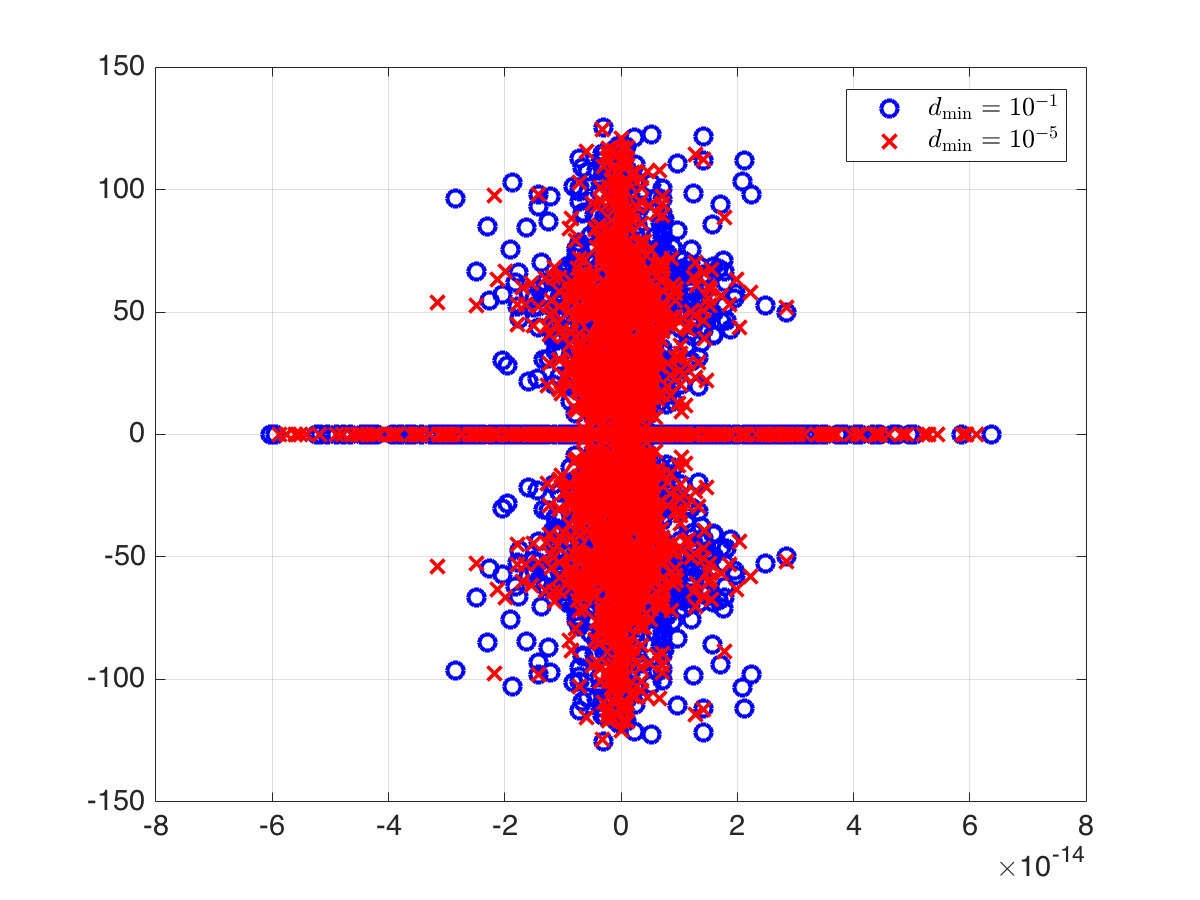
\includegraphics[width=.475\textwidth]{figs/spectra_tau0.png}}
%\hspace{1em}
\subfloat[$\tau_v = \tau_\sigma = 1$]{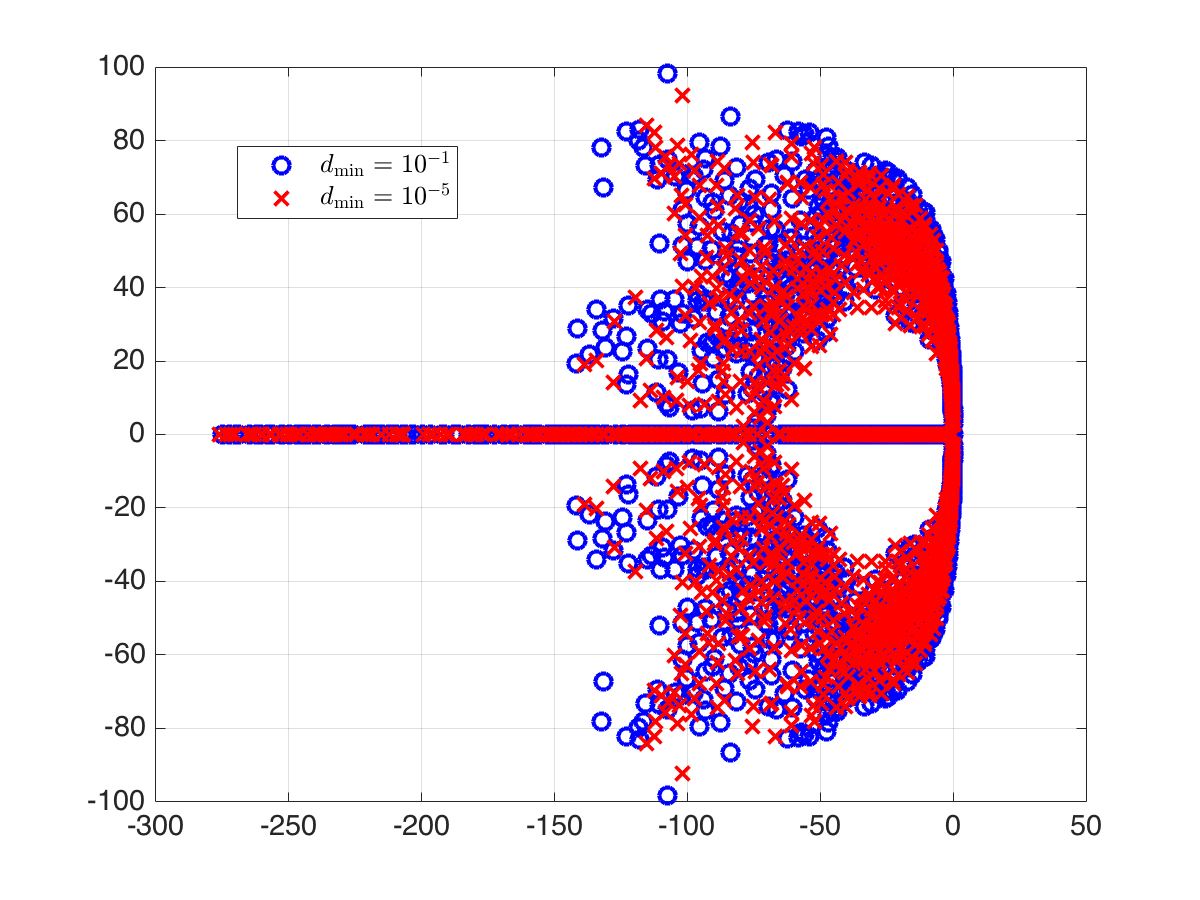
\includegraphics[width=.475\textwidth]{figs/spectra_tau1.png}}
\caption{Spectra for $N=4$ and $h = 1/4$, using randomly chosen $\bm{C}(\bm{x})$ with eigenvalues between $[d_{\min}, 1]$ at each quadrature point.  For both $\tau_v = \tau_\sigma = 0$ and $\tau_v = \tau_\sigma = 1$, the largest real part of the spectra is $O(10^{-14})$.}
\label{fig:spectra}
\end{figure}

For practical simulations, the choice of $\tau_v, \tau_\sigma$ remains to be specified.  Increasing $\tau_v,\tau_\sigma$ results in greater damping of under-resolved spurious components of the solution \cite{chan2016short}; however, a naive selection of these penalty parameters can result in an overly restrictive time-step restriction for stability.  We wish to choose $\tau_v,\tau_\sigma$ as large as possible without increasing $\nor{\bm{A}_h}$.  

To avoid artificially increasing the stiffness of (\ref{eq:wadgmat}), it was argued in \cite{chan2016short} that the magnitude of the penalty parameter should depend on the largest singular value of $\bm{A}_n$, which is $O(1)$ in two and three dimensions.  However, this suggestion does not factor in the effect of $\rho$ and $\bm{C}^{-1}$ appearing in the left hand side.  These material coefficients can be taken into account by scaling the penalty parameters such that flux terms are dimensionally consistent.  One example of such a scaling is
\[
\tau_v = \gamma_v \sup_{\bm{x} \in f} \sqrt{\nor{\avg{\bm{C}(\bm{x})}}\avg{\rho(\bm{x})}}, \qquad \tau_\sigma =  \gamma_\sigma  \sup_{\bm{x} \in f} \frac{1}{\sqrt{\nor{\avg{\bm{C}(\bm{x})}}\avg{\rho(\bm{x})}}},
\]  
where the supremum is taken locally over each face and $\gamma_v, \gamma_\sigma$ are dimensionless constants.  %We adopt this scaling for all remaining experiments, with $\gamma_v = 1/2$, $\gamma_\sigma = 1$ 

% 


%We note that, for $\tau_v = \tau_\sigma = 1$, $\nor{\bm{A}_h}$ is over twice as large compared to when $\tau_v = \tau_\sigma = 0$.   This can result in a more restrictive stability condition on the time-step.  We observe that the growth in $\nor{\bm{A}_h}$ for $\tau_v,\tau_\sigma = 1$ is due to the presence of eigenvalues with large negative real parts, which suggests that larger time-steps may be used under time integrators with extended stability regions along the real axis \cite{abdulle2002fourth}.  

%Under this scaling, taking $\gamma_v = 1, \gamma_\sigma / d$, where $d$ is the spatial dimension 

%These coefficients can be taken into account by scaling only the stress penalization parameter with the average of local max norms over a face $f$
%\[
%\tau_{\sigma,f} \approx \frac{2}{\nor{\bm{C}^+(\bm{x})}_{2,\infty,f}+\nor{\bm{C}^-(\bm{x})}_{2,\infty,f}},
%\]
%where $\bm{C}^+,\bm{C}^-$ denote values of the stiffness matrix on elements which share the face $f$.  It may also be advantageous to rescale $\tau_\sigma$ for each individual component of stress based on the rows of $\bm{C}$.  Under this rescaling of the stress penalty parameter, we observe numerically that the norm of $\bm{A}_h$ remains roughly the same magnitude as for $\tau_p = \tau_\sigma = 0$.   We do not observe significant changes in computed $L^2$ errors under the aforementioned rescaling of $\tau_\sigma$.  



\subsection{Analytic solutions} 

Next, we study the accuracy and convergence of weight-adjusted DG method for several analytical solutions in linear elasticity.  In all cases, the solution is expressed terms of the displacement vector $\bm{u}(\bm{x},t) = (u_1,\ldots,u_d)$.  Initial conditions for velocity and stress are computed through 
\[
\bm{v}(\bm{x},t) = \pd{\bm{u}}{t}, \qquad \bm{\sigma} = \bm{C}\frac{1}{2}\LRp{\Grad\bm{u} + \Grad\bm{u}^T}.  
\]
Unless otherwise stated, we report relative $L^2$ errors for all components of the solution $\bm{U} = (\bm{v},\bm{\sigma})$ 
\[
\frac{\nor{\bm{U}-\bm{U}_h}_{L^2\LRp{\Omega}}}{\nor{\bm{U}}_{L^2\LRp{\Omega}}} = \frac{\LRp{\sum_{i=1}^m \nor{\bm{U}_i-\bm{U}_{i,h}}^2_{L^2\LRp{\Omega}}}^{1/2}}{\LRp{\sum_{i=1}^m\nor{\bm{U}_i}^2_{L^2\LRp{\Omega}}}^{1/2}}.
\]

\subsubsection{Harmonic oscillation of a square} 

We first examine convergence  on a unit square domain with  $\lambda = \mu = \rho = 1$.   The components of the displacement vector are given by
\begin{align*}
u_1(x,y,t) &= \cos(\omega\pi t)\cos(\pi x)\sin(\pi y)\\
u_2(x,y,t) &= -\cos(\omega\pi t)\sin(\pi x)\cos(\pi y),
\end{align*}
where $\omega = \sqrt{2\mu}$.  Zero traction boundary conditions are imposed.  Figure~\ref{fig:harmonic_osc} shows $L^2$ errors computed at time $T = 5$, using uniform triangular meshes constructed by bisecting a uniform mesh of quadrilaterals along the diagonal.  For $N = 1,\ldots, 5$, rates near the optimal $O(h^{N+1})$ rates of convergence are observed.  

\begin{figure}
\centering
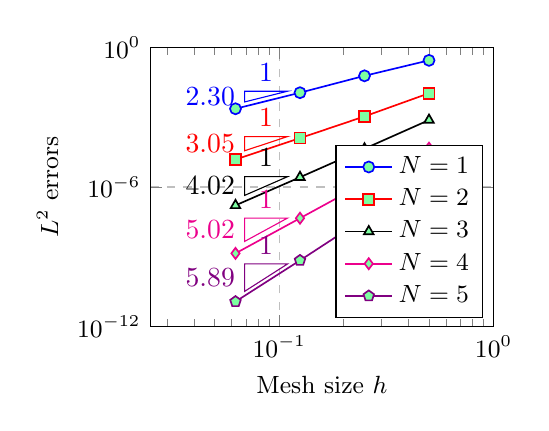
\begin{tikzpicture}
\begin{loglogaxis}[
	legend cell align=left,
	width=.49\textwidth,
    xlabel={Mesh size $h$},
       ylabel={$L^2$ errors}, 
    xmin=.025, xmax=1,
    ymin=1e-12, ymax=1,
    legend pos=south east,
    xmajorgrids=true,
    ymajorgrids=true,
    grid style=dashed,
] 

\addplot[color=blue,mark=*,semithick, mark options={fill=markercolor}]
coordinates{(0.5,0.281186)(0.25,0.0607224)(0.125,0.0114231)(0.0625,0.00232631)};
\logLogSlopeTriangleFlip{0.4}{0.125}{0.805}{2.30}{blue}

\addplot[color=red,mark=square*,semithick, mark options={fill=markercolor}]
coordinates{(0.5,0.010807)(0.25,0.00109063)(0.125,0.000126864)(0.0625,1.53214e-05)};
\logLogSlopeTriangleFlip{0.4}{0.125}{0.63}{3.05}{red}

\addplot[color=black,mark=triangle*,semithick, mark options={fill=markercolor}]
coordinates{(0.5,0.000760654)(0.25,4.44169e-05)(0.125,2.63258e-06)(0.0625,1.62546e-07)};
\logLogSlopeTriangleFlip{0.4}{0.125}{0.47}{4.02}{black}

\addplot[color=magenta,mark=diamond*,semithick, mark options={fill=markercolor}]
coordinates{(0.5,4.68589e-05)(0.25,1.48545e-06)(0.125,4.55009e-08)(0.0625,1.39823e-09)};
\logLogSlopeTriangleFlip{0.4}{0.125}{0.305}{5.02}{magenta}

\addplot[color=violet,mark=pentagon*,semithick, mark options={fill=markercolor}]
coordinates{(0.5,3.03577e-06)(0.25,4.50412e-08)(0.125,6.98053e-10)(0.0625,1.17913e-11)};
\logLogSlopeTriangleFlip{0.4}{0.125}{0.126}{5.89}{violet}

\legend{$N=1$,$N=2$,$N=3$,$N=4$,$N=5$}
\end{loglogaxis}
\end{tikzpicture}
\caption{Convergence of $L^2$ errors for harmonic oscillation.}
\label{fig:harmonic_osc}
\end{figure}

\subsubsection{Rayleigh and Lamb waves}  

Next, we examine the convergence of WADG for Rayleigh and Lamb waves, both of which test the imposition of traction-free boundary conditions.  

Rayleigh waves are elastic surface waves which decay exponentially away from the surface.  These waves are given by the displacement vector
\begin{align*}
\bm{u}\LRp{x,y,t} &= e^{-\omega x \sqrt{1-\xi^2}}
\LRp{
\begin{array}{c}
\cos(\omega(y+c_r t)) \\
\sqrt{1-\xi^2}\sin(\omega(y+c_r t))
\end{array}
}\\
&+ \LRp{\frac{\xi^2}{2}-1}e^{-\omega x\sqrt{1-\frac{\xi^2\mu}{2\mu + \lambda}}}
\LRp{
\begin{array}{c}
\cos(\omega(y + c_r t))\\
{\sin(\omega(y+c_r t))}/{\sqrt{1-\frac{\xi^2\mu}{2\mu + \lambda}}}
\end{array}
},
\end{align*}
where $\omega$ is the wavespeed, $c_r$ is the Rayleigh phase velocity $c_r = \xi \sqrt{\mu}$, and $\xi$ satisfies
\[
\sqrt{1-\xi^2}\sqrt{1 - \frac{\xi^2\mu}{2\mu+\lambda}} - \LRp{\frac{\xi^2}{2}-1}^2 = 0.
\]
In our computations, we use $\rho = \mu = \lambda = 1$, $\xi = 0.949554083888034$, and $\omega = 2\pi$ \cite{wilcox2010high}.  We solve on the domain $[0,2]\times[0,1]$ using a sequence of uniform triangular meshes, and enforce traction-free boundary conditions at $x=0$ and exact Dirichlet boundary conditions at $x=2$.  Periodic boundary conditions are applied at $y = 0$ and $y = 1$.  

Lamb waves are supported by elastic waveguides with traction-free (free surface) boundary conditions at the top and bottom of the domain.  The displacement of these waves is given by
\begin{align*}
{u}_1\LRp{x,y,t} &= \LRp{-kB_1 \cos(p y)- qB_2 \cos(q y)} \sin(k x - \omega t)\\
{u}_2\LRp{x,y,t} &= \LRp{-pB_1 \sin(py) + kB_2 \sin(qy)} \cos(kx - \omega t)
\end{align*}
where $k$ is the wavenumber and $\omega$ is the frequency, and the constants $p$ and $q$ are defined as
\[
p^2 = \frac{\omega^2}{2\mu + \lambda} - k^2, \qquad q^2 = \frac{\omega^2}{\mu} - k^2.
\]
The wavenumber $k$ and frequency $\omega$ are related through a dispersion relation.  The ratio of the amplitudes $B_1/ B_2$ can be determined using other parameters, implying that $B_1, B_2$ are unique up to a scaling constant.  In our experiments, we use $\rho = \mu = 1$, $\lambda = 2$, $k = 2\pi$.  For these values, $\omega = 13.137063197233$, $B_1 = 126.1992721468$ and $B_2 = 53.88807700007$ \cite{wilcox2010high}.  We solve on the domain $[-1,1]\times[-1/2,1/2]$, with traction-free boundary conditions at $y = \pm 1/2$ and periodic boundary conditions at $x = \pm 1$.  

Figure~\ref{fig:rayleigh} shows $L^2$ errors for both waves at time $T = 5$.  Computed convergence rates fall between the optimal rate of $O(h^{N+1})$ and theoretical rate of $O(h^{N+1/2})$ \cite{johnson1986analysis}.  

\begin{figure}
\centering
\subfloat[Rayleigh wave]{
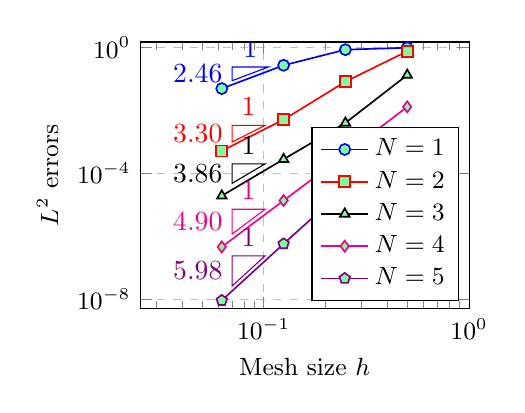
\begin{tikzpicture}
\begin{loglogaxis}[
    legend cell align=left,
    width=.475\textwidth,
    xlabel={Mesh size $h$},
    ylabel={$L^2$ errors}, 
    xmin=.025, xmax=1,
    ymin=5e-9, ymax=1.5,
    legend pos=south east,
    xmajorgrids=true,
    ymajorgrids=true,
    grid style=dashed,
] 

\addplot[color=blue,mark=*,semithick, mark options={fill=markercolor}]
coordinates{(0.5,0.987525)(0.25,0.856084)(0.125,0.272343)(0.0625,0.0495455)};
\logLogSlopeTriangleFlip{.39}{0.11}{0.855}{2.46}{blue}

\addplot[color=red,mark=square*,semithick, mark options={fill=markercolor}]
coordinates{(0.5,0.762022)(0.25,0.0822137)(0.125,0.00510445)(0.0625,0.000517961)};
\logLogSlopeTriangleFlip{.38}{0.1}{0.625}{3.30}{red}

\addplot[color=black,mark=triangle*,semithick, mark options={fill=markercolor}]
coordinates{(0.5,0.133471)(0.25,0.00400974)(0.125,0.000280342)(0.0625,1.93442e-05)};
\logLogSlopeTriangleFlip{.38}{0.1}{0.47}{3.86}{black}

\addplot[color=magenta,mark=diamond*,semithick, mark options={fill=markercolor}]
coordinates{(0.5,0.0130378)(0.25,0.000405004)(0.125,1.36821e-05)(0.0625,4.57998e-07)};
\logLogSlopeTriangleFlip{.38}{0.1}{0.28}{4.90}{magenta}

\addplot[color=violet,mark=pentagon*,semithick, mark options={fill=markercolor}]
coordinates{(0.5,0.00157091)(0.25,3.42541e-05)(0.125,5.7373e-07)(0.0625,9.09776e-09)};
\logLogSlopeTriangleFlip{.38}{0.1}{0.085}{5.98}{violet}

%\node at (axis cs:.03,6.8e-10) {$u$ discontinuous};
\legend{$N=1$,$N=2$,$N=3$,$N=4$,$N=5$}
\end{loglogaxis}
\end{tikzpicture}
}
\subfloat[Lamb wave]{
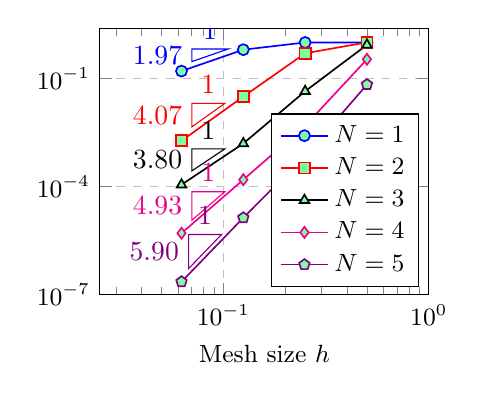
\begin{tikzpicture}
\begin{loglogaxis}[
	legend cell align=left,
	width=.475\textwidth,
    xlabel={Mesh size $h$},
%       ylabel={$L^2$ errors}, 
    xmin=.025, xmax=1,
    ymin=1e-7, ymax=2.5,
    legend pos=south east,
    xmajorgrids=true,
    ymajorgrids=true,
    grid style=dashed,
] 

\addplot[color=blue,mark=*,semithick, mark options={fill=markercolor}]
coordinates{(0.5,1.00019)(0.25,1.00515)(0.125,0.633842)(0.0625,0.161762)};
\logLogSlopeTriangleFlip{.39}{0.11}{0.875}{1.97}{blue}

\addplot[color=red,mark=square*,semithick, mark options={fill=markercolor}]
coordinates{(0.5,1.01296)(0.25,0.503696)(0.125,0.0316637)(0.0625,0.00188428)};
\logLogSlopeTriangleFlip{.38}{0.1}{0.63}{4.07}{red}

\addplot[color=black,mark=triangle*,semithick, mark options={fill=markercolor}]
coordinates{(0.5,0.865781)(0.25,0.0445608)(0.125,0.00158453)(0.0625,0.000113704)};
\logLogSlopeTriangleFlip{.38}{0.1}{0.465}{3.80}{black}

\addplot[color=magenta,mark=diamond*,semithick, mark options={fill=markercolor}]
coordinates{(0.5,0.343325)(0.25,0.00491357)(0.125,0.000156595)(0.0625,5.13222e-06)};
\logLogSlopeTriangleFlip{.38}{0.1}{0.28}{4.93}{magenta}

\addplot[color=violet,mark=pentagon*,semithick, mark options={fill=markercolor}]
coordinates{(0.5,0.0682545)(0.25,0.000718077)(0.125,1.37715e-05)(0.0625,2.30844e-07)};
\logLogSlopeTriangleFlip{0.37}{0.1}{0.0985}{5.90}{violet}

\legend{$N=1$,$N=2$,$N=3$,$N=4$,$N=5$}
\end{loglogaxis}
\end{tikzpicture}
}
\caption{Convergence of $L^2$ errors for Rayleigh and Lamb wave solutions.}
\label{fig:rayleigh}
\end{figure}

\subsubsection{Rayleigh waves in near-incompressible materials}
\label{sec:incomp}

As noted in Section~\ref{sec:wadgelas}, error estimates for isotropic elasticity no longer hold in the incompressible limit $\mu / \lambda \rightarrow 0$ due to the fact that $\bm{C}$ becomes singular.  We use the propagation of Rayleigh waves to examine the behavior of WADG for near-incompressible materials.  We follow \cite{sjogreen2012fourth, appelo2015energy} and fix $\lambda = 1$ and set $\mu = 1, .1, .01, .001, .0001$.  Since the Rayleigh wave propagates with speed proportional to $\sqrt{\mu}$, we compute $L^2$ errors at the final time $1 / (4\sqrt{\mu})$ to ensure a fair comparison between solutions at different values of $\mu$.  

%Table~\ref{tab:incomp} shows total relative errors and relative errors for $\bm{v}$, $\bm{\sigma}$ individually at different orders and mesh sizes.  While the relative errors for $\bm{\sigma}$ grow as $\mu/\lambda \rightarrow 0$, total errors and errors for $\bm{v}$ remain roughly the same magnitude for all values of $\mu$.  
Table~\ref{tab:incomp} shows relative errors for $\bm{v}$, $\bm{\sigma}$ at different orders and mesh sizes.  The relative errors for $\bm{\sigma}$ grow as $\mu/\lambda \rightarrow 0$.  This is not surprising, as the constant in the error estimates of Section~\ref{sec:mwadgprop} depends on $\nor{\bm{C}}$, which blows up in the incompressible limit.  However, because the magnitude of $\bm{\sigma}$ also decreases as $\mu/\lambda\rightarrow 0$, relative errors for $\bm{v}$ remain roughly the same magnitude for near-incompressible materials.  Decreasing $\mu$ by four orders of magnitude results in up to a ten-fold increase in relative error for $\bm{\sigma}$, but less than a two-fold increase in error for $\bm{v}$.  

\begin{table}
\centering
\subfloat[Relative error in $\bm{v}$]{
\begin{tabular}{|c||c|c|c|c|c|}
\hline
 & $\mu = 1$ & $\mu = .1$ & $\mu = .01$ & $\mu = .001$ & $\mu = .0001$  \\
\hhline{|=|=|=|=|=|=|}
$N = 2$, $h = 1/4$ &  3.1063e-02  &  2.6972e-02  & 3.0858e-02 &  4.0103e-02  & 5.6835e-02\\
\hline
$N = 3$, $h = 1/4$ & 3.1677e-03 &  2.6848e-03 &  2.9854e-03 &  3.6960e-03 &  4.9362e-03\\
\hline
$N = 4$, $h = 1/4$ & 2.8726e-04 &  2.4990e-04 &  2.9142e-04 &  3.9774e-04 &  5.2469e-04\\      

\hhline{|=|=|=|=|=|=|}
$N = 2$, $h = 1/8$ & 3.1819e-03  & 2.5476e-03 &  2.8877e-03 &  3.5608e-03  & 4.7010e-03 \\
\hline
$N = 3$, $h = 1/8$ & 1.8867e-04  & 1.6925e-04  & 1.8509e-04  & 2.2520e-04  & 2.8301e-04\\
\hline
$N = 4$, $h = 1/8$ & 8.4999e-06  & 7.5750e-06 &  8.1094e-06  & 1.0760e-05  & 1.4886e-05\\
\hline         
\end{tabular}
}\\
\subfloat[Relative error in $\bm{\sigma}$]{
\begin{tabular}{|c||c|c|c|c|c|}
\hline
 & $\mu = 1$ & $\mu = .1$ & $\mu = .01$ & $\mu = .001$& $\mu = .0001$ \\
\hhline{|=|=|=|=|=|=|}
$N = 2$, $h = 1/4$ & 6.8250e-02  & 7.4130e-02 &  1.2104e-01 &  2.1333e-01 &  4.1451e-01\\
\hline
$N = 3$, $h = 1/4$ & 9.2980e-03  & 1.0685e-02 &  1.8109e-02 &  3.2046e-02 &  5.7612e-02\\
\hline
$N = 4$, $h = 1/4$ & 9.7251e-04  & 1.1687e-03  & 2.1941e-03 &  4.1378e-03 &  6.8404e-03\\
\hhline{|=|=|=|=|=|=|}
$N = 2$, $h = 1/8$ & 9.8138e-03  & 1.1429e-02  & 2.0331e-02 &  3.7889e-02 & 7.6516e-02\\
\hline
$N = 3$, $h = 1/8$ & 6.6596e-04  & 7.8157e-04  & 1.5353e-03  & 3.1239e-03 &  5.6341e-03\\
\hline
$N = 4$, $h = 1/8$ & 3.4272e-05  & 4.2639e-05 &  8.8393e-05  & 1.9764e-04 &  3.6052e-04 \\
\hline
\end{tabular}
}
%\\
%\subfloat[Total relative error ]{
%\begin{tabular}{|c||c|c|c|c|c|}
%\hline
% & $\mu = 1$ & $\mu = .1$ & $\mu = .01$ & $\mu = .001$ & \mu = .0001$ \\
%\hhline{|=|=|=|=|=|=|}
%$N = 2$, $h = 1/4$ & 0.0539 & 0.0369  &  0.0339 & 0.0409 & 0.0571\\
%\hline
%$N = 3$, $h = 1/4$ & 0.0073 & 0.0046 &0.0037 &0.0039 & 0.0050\\
%\hline
%$N = 4$, $h = 1/4$ & 7.7419e-04 & 4.8735e-04 & 3.9193e-04 &4.2768e-04 &5.3111e-04\\
%\hhline{|=|=|=|=|=|=|}
%$N = 2$, $h = 1/8$ & 0.0074 & 0.0048  & 0.0038 &  0.0038 & 0.0048  \\
%\hline
%$N = 3$, $h = 1/8$ & 5.4120e-04 & 3.2760e-04 &2.6070e-04 & 2.5465e-04 & 2.9104e-04\\
%\hline
%$N = 4$, $h = 1/8$ & 2.7006e-05 & 1.7103e-05 &1.3344e-05 &1.3133e-05&1.5507e-05\\
%\hline
%\end{tabular}
%}
\caption{Behavior of WADG for linear elastic wave propagation in the incompressible limit as $\mu / \lambda \rightarrow 0$.  Errors are shown for various orders and mesh resolutions.  }
\label{tab:incomp}
\end{table}

\subsubsection{Stoneley waves} 

A Stoneley wave is supported along the interface between two solids \cite{stoneley1924elastic}.  Like Rayleigh waves, Stoneley waves decay exponentially away from the interface, and test the effectiveness of numerical fluxes across interfaces.  We follow \cite{wilcox2010high,appelo2015energy} and use discontinuous media defined by
\[
(\rho,\lambda,\mu) = \begin{cases}
(10 ,3,3) & y > 0\\
(1,1,1) & y < 0.
\end{cases}.
\]
The displacement vector for a Stoneley wave is then given by
\begin{align*}
u_1(x,y,t) &= \begin{cases}
{\rm Re}\LRp{\LRp{ikB_1e^{-kb_{1p}y} + kb_{1s}B_2 e^{-kb_{1s}y}}e^{i(ky-\omega t)}}, & y > 0\\
{\rm Re}\LRp{\LRp{-k b_{1p}B_1e^{-k b_{1p} y} + i kB_2e^{-kb_{1s}y}}e^{i(kx-\omega t)}}, & y < 0
\end{cases}\\
u_2(x,y,t) &= \begin{cases}
{\rm Re}\LRp{\LRp{ikB_3 e^{k b_{2p} y} - kb_{2s}B_4 e^{k b_{2s}y }} e^{i(kx-\omega t)}}, & y > 0\\
{\rm Re}\LRp{\LRp{k b_{2p} B_3 e^{k b_{2p}y} + ikB_4 e^{k b_{2s}y}}e^{i(kx-\omega t)}}, & y < 0
\end{cases},
\end{align*}
where $c_{st}$ is the Stoneley wave speed, and 
\[
k = \omega/ c_{st}, \qquad b_{jp} = \sqrt{1 - \frac{c_{st}^2}{(2\mu_j + \lambda_j)/\rho_j}}, \qquad  b_{js} = \sqrt{1 - \frac{c_{st}^2}{(\mu_j)/\rho_j}}, \qquad j = 1,2.
\]
The Stoneley wave speed $c_{st}$ can be determined based material parameters and interface conditions, and the amplitudes $B_1,B_2,B_3,B_4$ are determined from $c_{st}$ up to scaling by a constant.  For the parameters used in this study, we take $c_{st} = 0.546981324213884$, $B_1 = i0.2952173626624, B_2 = -0.6798795208473, B_3 = i0.5220044931212$, and $B_4 = -0.9339639688697$ \cite{wilcox2010high}.  We assume $k =1$, which gives $\omega=c_{st}$.  

We solve on the domain $[-1,1]\times [-5,5]$, and enforce Dirichlet boundary conditions at all boundaries using the exact solution.  Figure~\ref{fig:stoneley} shows $L^2$ errors for two uniform meshes of triangles constructed by bisecting a quadrilateral mesh of $K_{\rm 1D} \times 5K_{\rm 1D}$ elements. Figure~\ref{subfig:stoneley1} shows errors at time $T=5$ when $K_{\rm 1D}$ is even and the mesh is fitted to the interface at $y = 0$, while Figure~\ref{subfig:stoneley2} shows errors when $K_{\rm 1D}$ is odd and the interface cuts through element interiors.  

When the mesh is fitted to the interface, computed convergence rates match the estimated $O(h^{N+1/2})$ rate.  When the mesh is not fitted to the interface exactly, we compute the application of the weight-adjusted mass matrix inverse using a quadrature rule from Xiao and Gimbutas \cite{xiao2010quadrature} which is exact for degree $2N+1$ polynomials.  Since the values of $\rho,\mu$, and $\lambda$ are positive at all quadrature points, the method is energy stable.  However, since the exact solution is discontinuous, the error in elements cut by the interface is $O(1)$, resulting in $L^2$ errors which converge at rate $O(h^{1/2})$.  We note that, when using piecewise constant approximations of $\mu$ and $\lambda$, we observe the same $O(h^{1/2})$ convergence rate, though errors are roughly twice as large in magnitude.  

\begin{figure}
\centering
\subfloat[Fitted interface]{
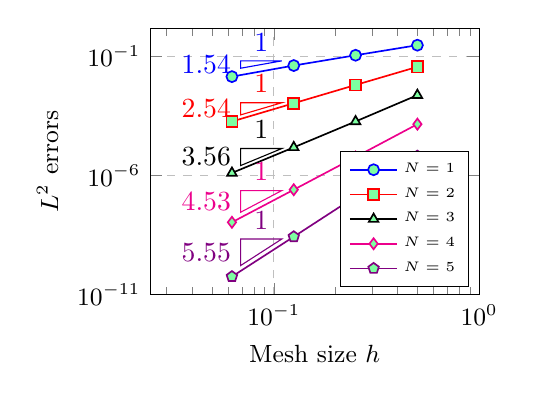
\begin{tikzpicture}
\begin{loglogaxis}[
    legend cell align=left,
    legend style={legend pos=south east, font=\tiny},
    width=.475\textwidth,
    xlabel={Mesh size $h$},
    ylabel={$L^2$ errors}, 
    xmin=.025, xmax=1,
    ymin=1e-11, ymax=1.5,
    xmajorgrids=true,
    ymajorgrids=true,
    grid style=dashed,
] 

\addplot[color=blue,mark=*,semithick, mark options={fill=markercolor}]
coordinates{(0.5,0.291816)(0.25,0.110431)(0.125,0.0409099)(0.0625,0.0140493)};
\logLogSlopeTriangleFlip{.4}{0.125}{0.85}{1.54}{blue}

\addplot[color=red,mark=square*,semithick, mark options={fill=markercolor}]
coordinates{(0.5,0.0360738)(0.25,0.00627358)(0.125,0.00107612)(0.0625,0.0001848)};
\logLogSlopeTriangleFlip{.4}{0.125}{0.675}{2.54}{red}

\addplot[color=black,mark=triangle*,semithick, mark options={fill=markercolor}]
coordinates{(0.5,0.00234802)(0.25,0.000185264)(0.125,1.51976e-05)(0.0625,1.28801e-06)};
\logLogSlopeTriangleFlip{.4}{0.125}{0.485}{3.56}{black}

\addplot[color=magenta,mark=diamond*,semithick, mark options={fill=markercolor}]
coordinates{(0.5,0.000142893)(0.25,5.99393e-06)(0.125,2.55178e-07)(0.0625,1.10265e-08)};
\logLogSlopeTriangleFlip{.4}{0.125}{0.31}{4.53}{magenta}

\addplot[color=violet,mark=pentagon*,semithick, mark options={fill=markercolor}]
coordinates{(0.5,6.55362e-06)(0.25,1.31822e-07)(0.125,2.7319e-09)(0.0625,5.82544e-11)};
\logLogSlopeTriangleFlip{0.4}{0.125}{0.11}{ 5.55}{violet}
%1.5419    2.5418    3.5606    4.5325    5.5514
%\node at (axis cs:.03,6.8e-10) {$u$ discontinuous};
\legend{$N=1$,$N=2$,$N=3$,$N=4$,$N=5$}
\end{loglogaxis}
\end{tikzpicture}
\label{subfig:stoneley1}
}
\subfloat[Non-fitted interface]{
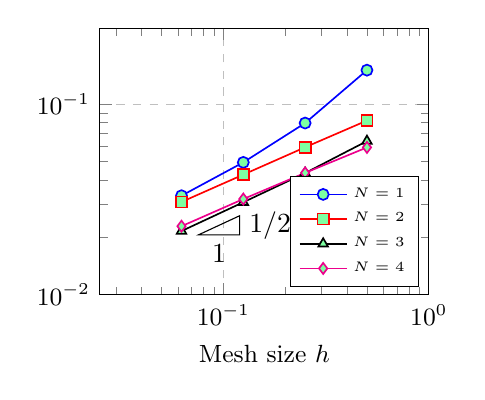
\begin{tikzpicture}
\begin{loglogaxis}[
    legend cell align=left,
    legend style={legend pos=south east, font=\tiny},
    width=.475\textwidth,
    xlabel={Mesh size $h$},
%    ylabel={$L^2$ errors}, 
    xmin=.025, xmax=1,
    ymin=1e-2, ymax=.25,
    xmajorgrids=true,
    ymajorgrids=true,
    grid style=dashed,
] 

\addplot[color=blue,mark=*,semithick, mark options={fill=markercolor}]
coordinates{(0.5,0.1507)(0.25,0.0796)(0.125,0.0495)(0.0625,0.0331)}; 
%\logLogSlopeTriangleFlip{0.32}{0.125}{0.84}{1}{blue}

\addplot[color=red,mark=square*,semithick, mark options={fill=markercolor}]
coordinates{(0.5,0.0820)(0.25,0.0594)(0.125,0.0427)(0.0625, 0.0307)};
%\logLogSlopeTriangleFlip{0.32}{0.125}{0.62}{3}{red}

\addplot[color=black,mark=triangle*,semithick, mark options={fill=markercolor}]
coordinates{(0.5, 0.0640)(0.25,0.0435)(0.125,0.0306)(0.0625,0.0216)};
%\logLogSlopeTriangleFlip{0.32}{0.125}{0.41}{4}{black}

\addplot[color=magenta,mark=diamond*,semithick, mark options={fill=markercolor}]
coordinates{(0.5, 0.0593)(0.25, 0.0436)(0.125, 0.0318)(0.0625,0.0229)};
\logLogSlopeTriangle{0.425}{0.125}{0.225}{1/2}{black}

%\node at (axis cs:.03,6.8e-10) {$u$ discontinuous};
\legend{$N=1$,$N=2$,$N=3$,$N=4$}
\end{loglogaxis}
\end{tikzpicture}
\label{subfig:stoneley2}
}
\caption{Convergence of WADG for a Stoneley wave using a fitted mesh aligned with the interface (Figure~\ref{subfig:stoneley1}) and a non-fitted mesh where the interface does not lie exactly on an element boundary (Figure~\ref{subfig:stoneley2}). }
\label{fig:stoneley}
\end{figure}

\subsubsection{Convergence to a reference solution}

Finally, we examine the accuracy of the WADG method for smoothly varying heterogeneous media by comparing against a reference spectral method solution with order $N = 50$ on a unit square $[-1,1]^2$.  Boundary conditions are enforced weakly through numerical fluxes \cite{wilcox2010high}.  We use a heterogeneous isotropic medium with $\rho,\lambda, \mu$ set to
\[
\rho(\bm{x}) = 1, \qquad \lambda(\bm{x}) = 1 + .25\sin(\pi x)\sin(\pi y), \qquad \mu(\bm{x}) = 1 + .25\cos(\pi x) \cos(\pi y).  
\]
Initial stresses are set to zero, while the initial velocity is set to 
\[
v_1(\bm{x}) = \cos(\pi x)\sin(\pi y), \qquad v_2(\bm{x}) = -\sin(\pi x)\cos(\pi y).
\]
Zero traction boundary conditions are enforced on all domain boundaries.  Figure~\ref{fig:refsol} shows $L^2$ errors with respect to the reference solution at time $T=1/2$ for different mesh sizes and orders of approximation.  Computed convergence rates fall between the optimal $O(h^{N+1})$ and predicted $O(h^{N+1/2})$.  
\begin{figure}
\centering
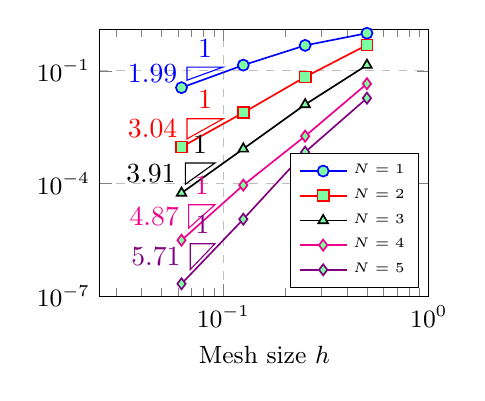
\begin{tikzpicture}
\begin{loglogaxis}[
    legend cell align=left,
    legend style={legend pos=south east, font=\tiny},
    width=.475\textwidth,
    xlabel={Mesh size $h$},
%    ylabel={$L^2$ errors}, 
    xmin=.025, xmax=1,
    ymin=1e-7, ymax=1.25,
    xmajorgrids=true,
    ymajorgrids=true,
    grid style=dashed,
] 

\addplot[color=blue,mark=*,semithick, mark options={fill=markercolor}]
coordinates{(0.5,1)(0.25,0.473741)(0.125,0.141342)(0.0625,0.0355409)};    
\logLogSlopeTriangleFlip{0.375}{0.11}{0.81}{1.99}{blue}

\addplot[color=red,mark=square*,semithick, mark options={fill=markercolor}]
coordinates{(0.5,0.484875)(0.25,0.0686547)(0.125,0.00767686)(0.0625,0.000933392)};   
\logLogSlopeTriangleFlip{0.375}{0.11}{0.59}{3.04}{red}

\addplot[color=black,mark=triangle*,semithick, mark options={fill=markercolor}]
coordinates{(0.5,0.141415)(0.25,0.0126263)(0.125,0.0008361)(0.0625,5.57276e-05)};    
\logLogSlopeTriangleFlip{0.35}{0.09}{0.42}{3.91}{black}

\addplot[color=magenta,mark=diamond*,semithick, mark options={fill=markercolor}]
coordinates{(0.5,0.0452398)(0.25,0.00182005)(0.125,9.0346e-05)(0.0625,3.08518e-06)};   
\logLogSlopeTriangleFlip{0.35}{0.08}{0.255}{4.87}{magenta}

\addplot[color=violet,mark=diamond*,semithick, mark options={fill=markercolor}]
coordinates{(0.5,0.0186937)(0.25,0.000684602)(0.125,1.12013e-05)(0.0625,2.13796e-07)};    
\logLogSlopeTriangleFlip{0.35}{0.075}{0.1}{5.71}{violet}

\legend{$N=1$,$N=2$,$N=3$,$N=4$,$N=5$}
\end{loglogaxis}
\end{tikzpicture}
\caption{Convergence of WADG under mesh refinement to a reference $N=50$ spectral method solution with smoothly varying heterogeneous media for $N=1,\ldots,5$.}
\label{fig:refsol}
\end{figure}

%\subsubsection{Harmonic oscillation of an annulus}
%
%This example tests the convergence of WADG for curvilinear mappings.  


\subsection{Application examples}

We next demonstrate the accuracy and flexibility of WADG for several application-based problems in linear elasticity with heterogeneity and anisotropy.  

\subsubsection{Stiff inclusion}

The stiff inclusion problem  is a common test of methods for linear elastic wave propagation \cite{leveque2002finite,kaser2006arbitrary,appelo2015energy}, where an inclusion with higher wavespeed is embedded within a non-stiff region.  Waves which reach this region of high wavespeed are transmitted through the inclusion, bouncing back and forth within the region.  This vibration then produces waves which propagate outward from the inclusion.  

We solve on a domain $[-1,1]\times [-.5, .5]$ with a rectangular inclusion located at $[-.5,.5]\times[-.1,.1]$.  Outside of the inclusion, material parameters are taken to be 
\[
\rho = 1, \qquad \mu = 1,\qquad \lambda = 2.
\]
Within the inclusion, material parameters are taken to be
\[
\rho = 1, \qquad \mu = 100,\qquad \lambda = 200,
\]
such that the wave speed in the rectangular inclusion is ten times that of the wave speed outside.  A pulse is generated through velocity boundary conditions at $x = -1$
\[
v_1(x,y,t) = \begin{cases}
\sin(\pi t / t_0), & t < t_0\\
0, & t \geq t_0
\end{cases}, \qquad
v_2(x,y,t) = 0.
\]
In our experiments, we take $t_0 = .025$.  Traction free boundary conditions are enforced at all other domain boundaries.  

\begin{figure}
\centering
\subfloat[$\LRb{\bm{\sigma}_{xx}+\bm{\sigma}_{yy}}$]{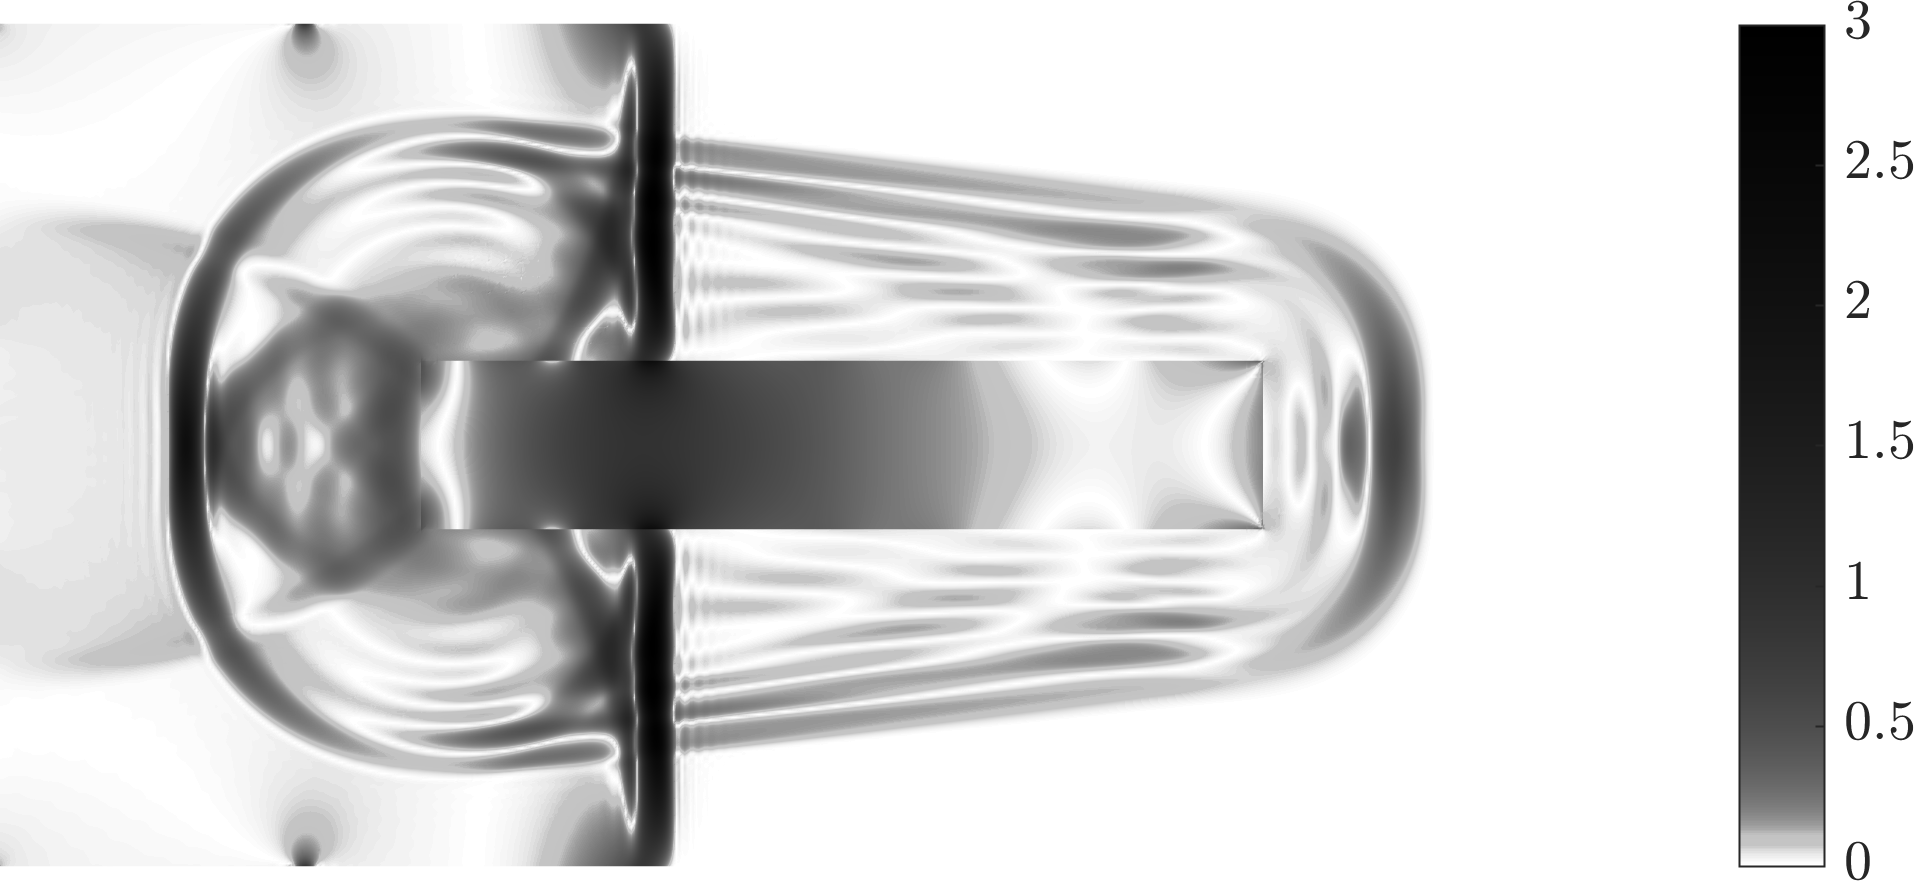
\includegraphics[width=.475\textwidth]{figs/inclusion_aligned.png}}
\hspace{2em}
\subfloat[$\LRb{\bm{\sigma}_{xy}}$]{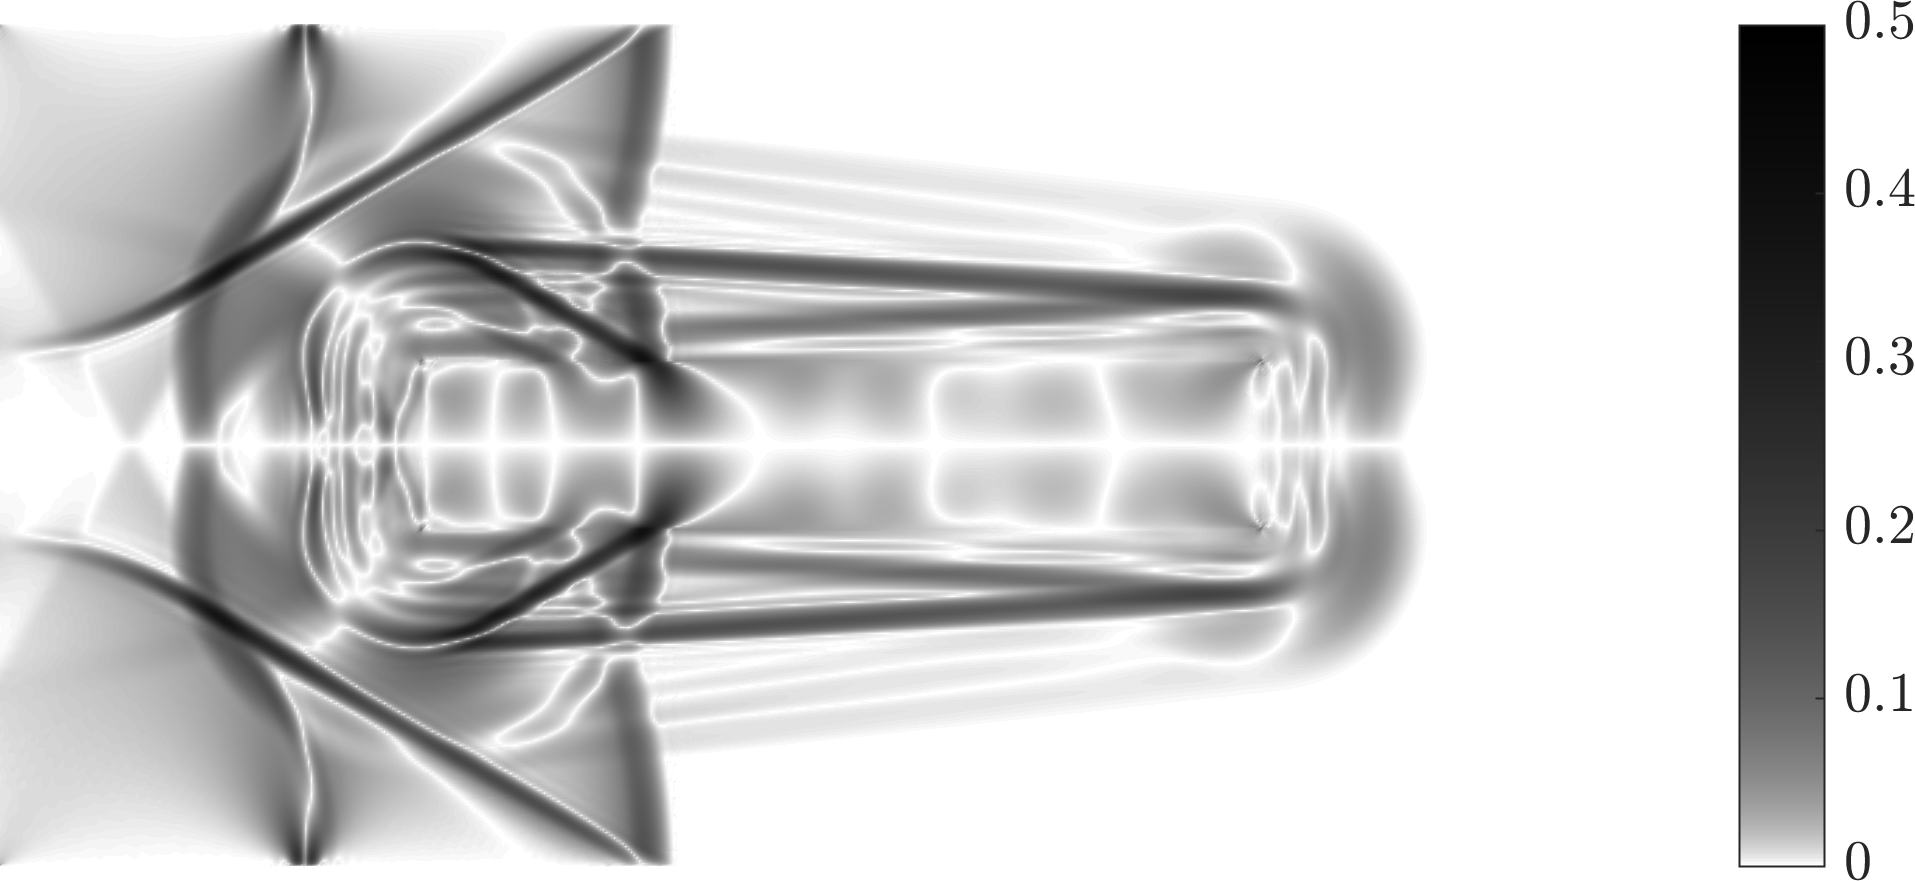
\includegraphics[width=.475\textwidth]{figs/inclusion_aligned_shear.png}}
%\subfloat[Aligned mesh (zoom)]{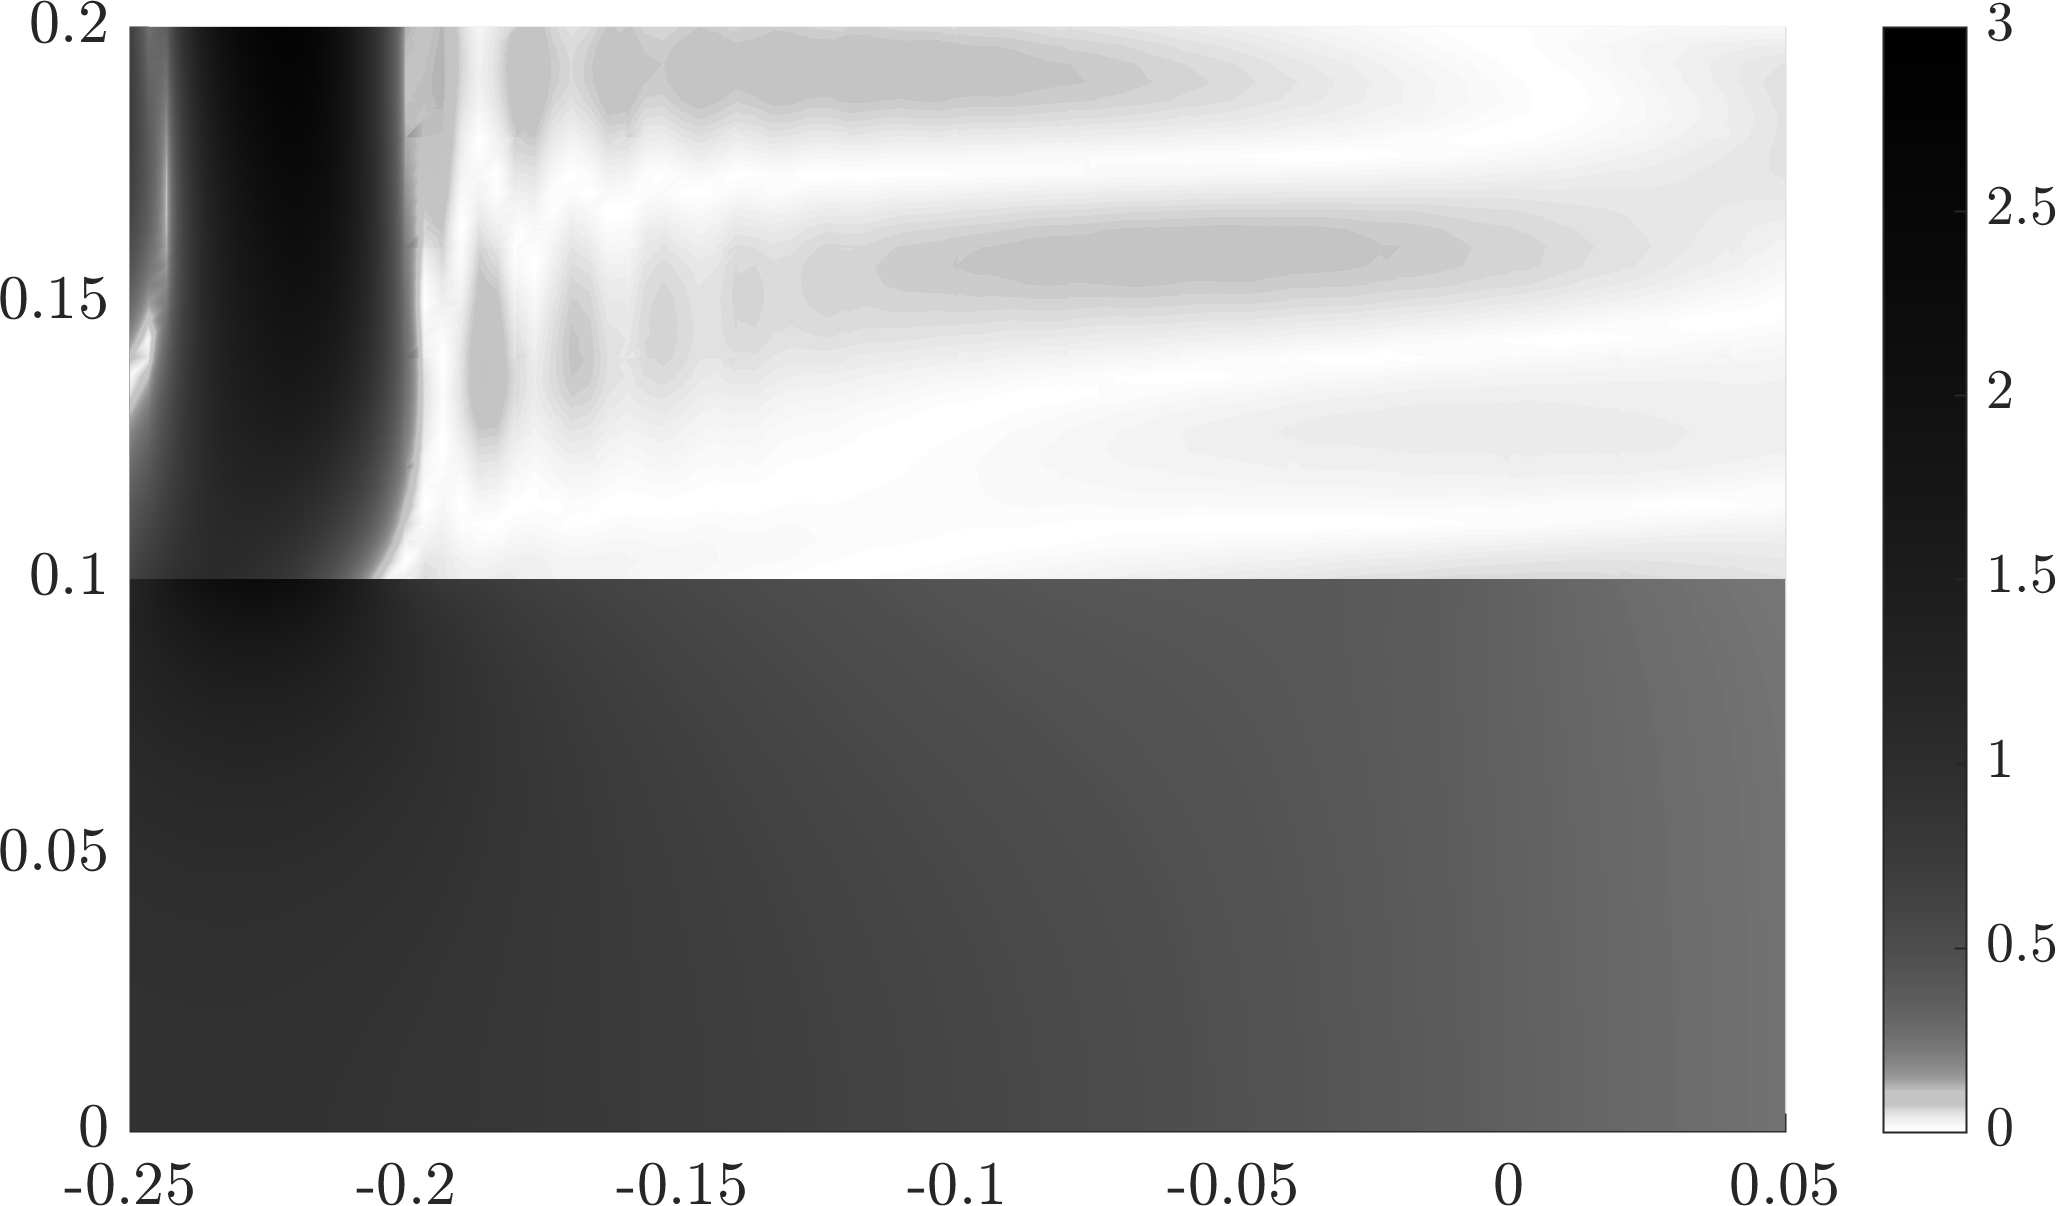
\includegraphics[height=.24\textwidth]{figs/inclusion_aligned_zoom.png}}
%\\
%\subfloat[Un-aligned mesh]{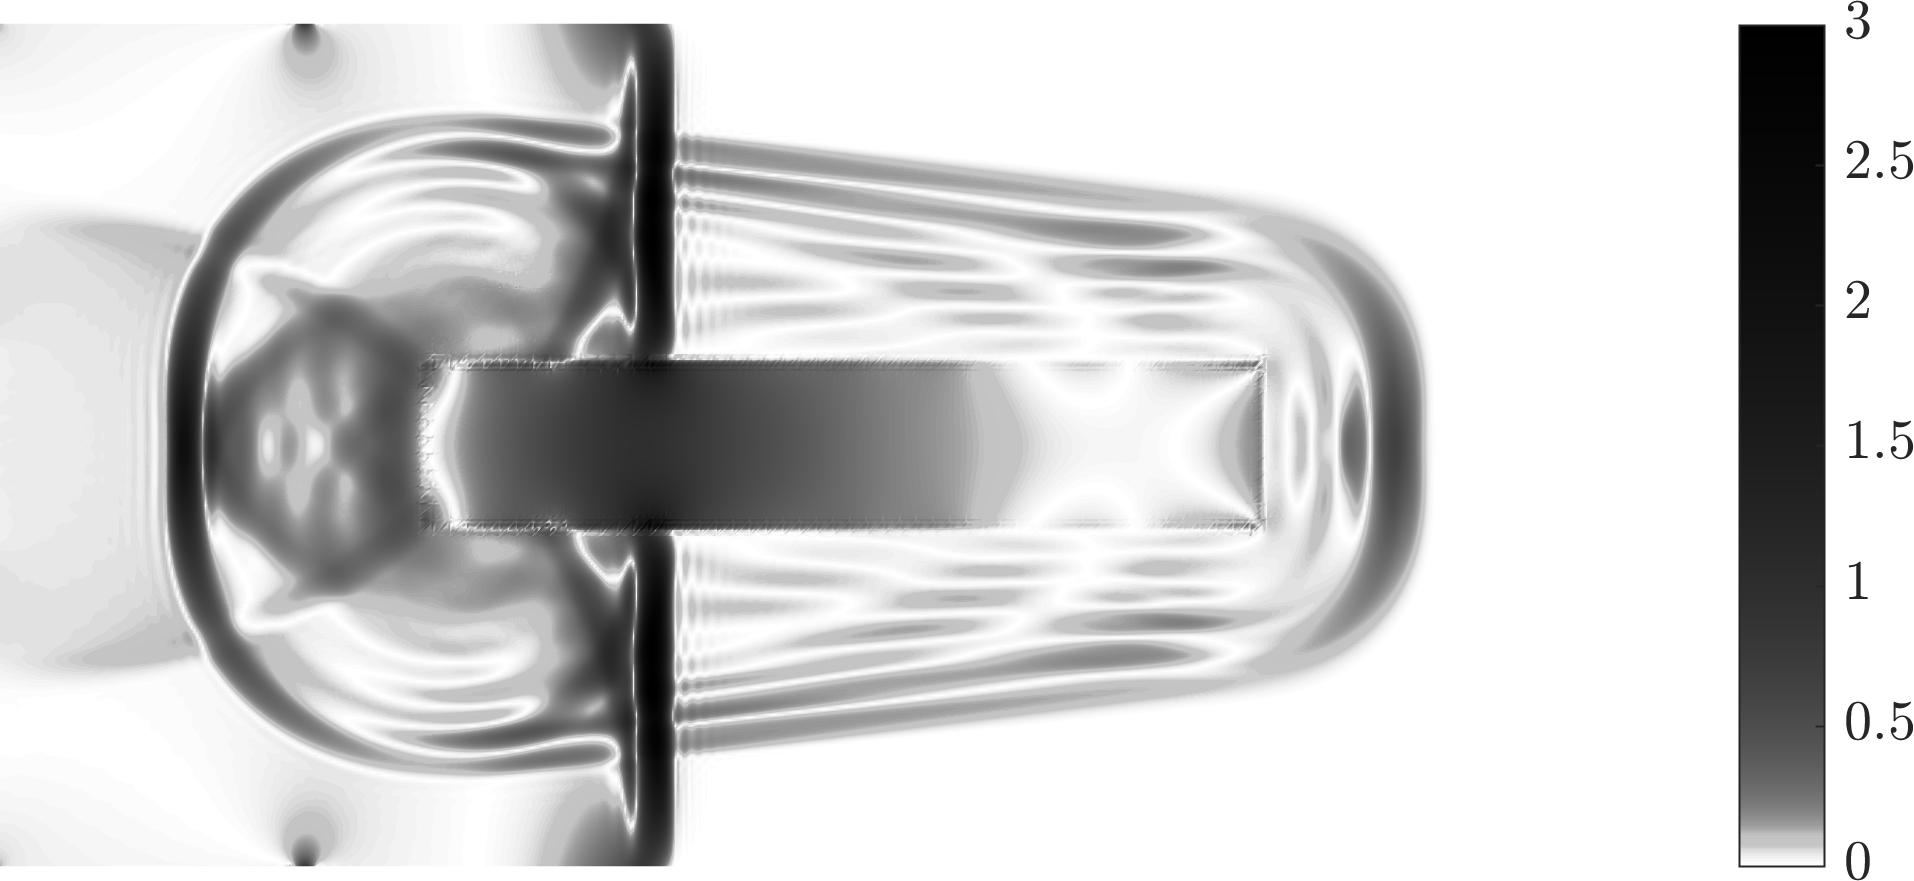
\includegraphics[height=.24\textwidth]{figs/inclusion_unaligned.png}}
%\hspace{2em}
%\subfloat[Un-aligned mesh (zoom)]{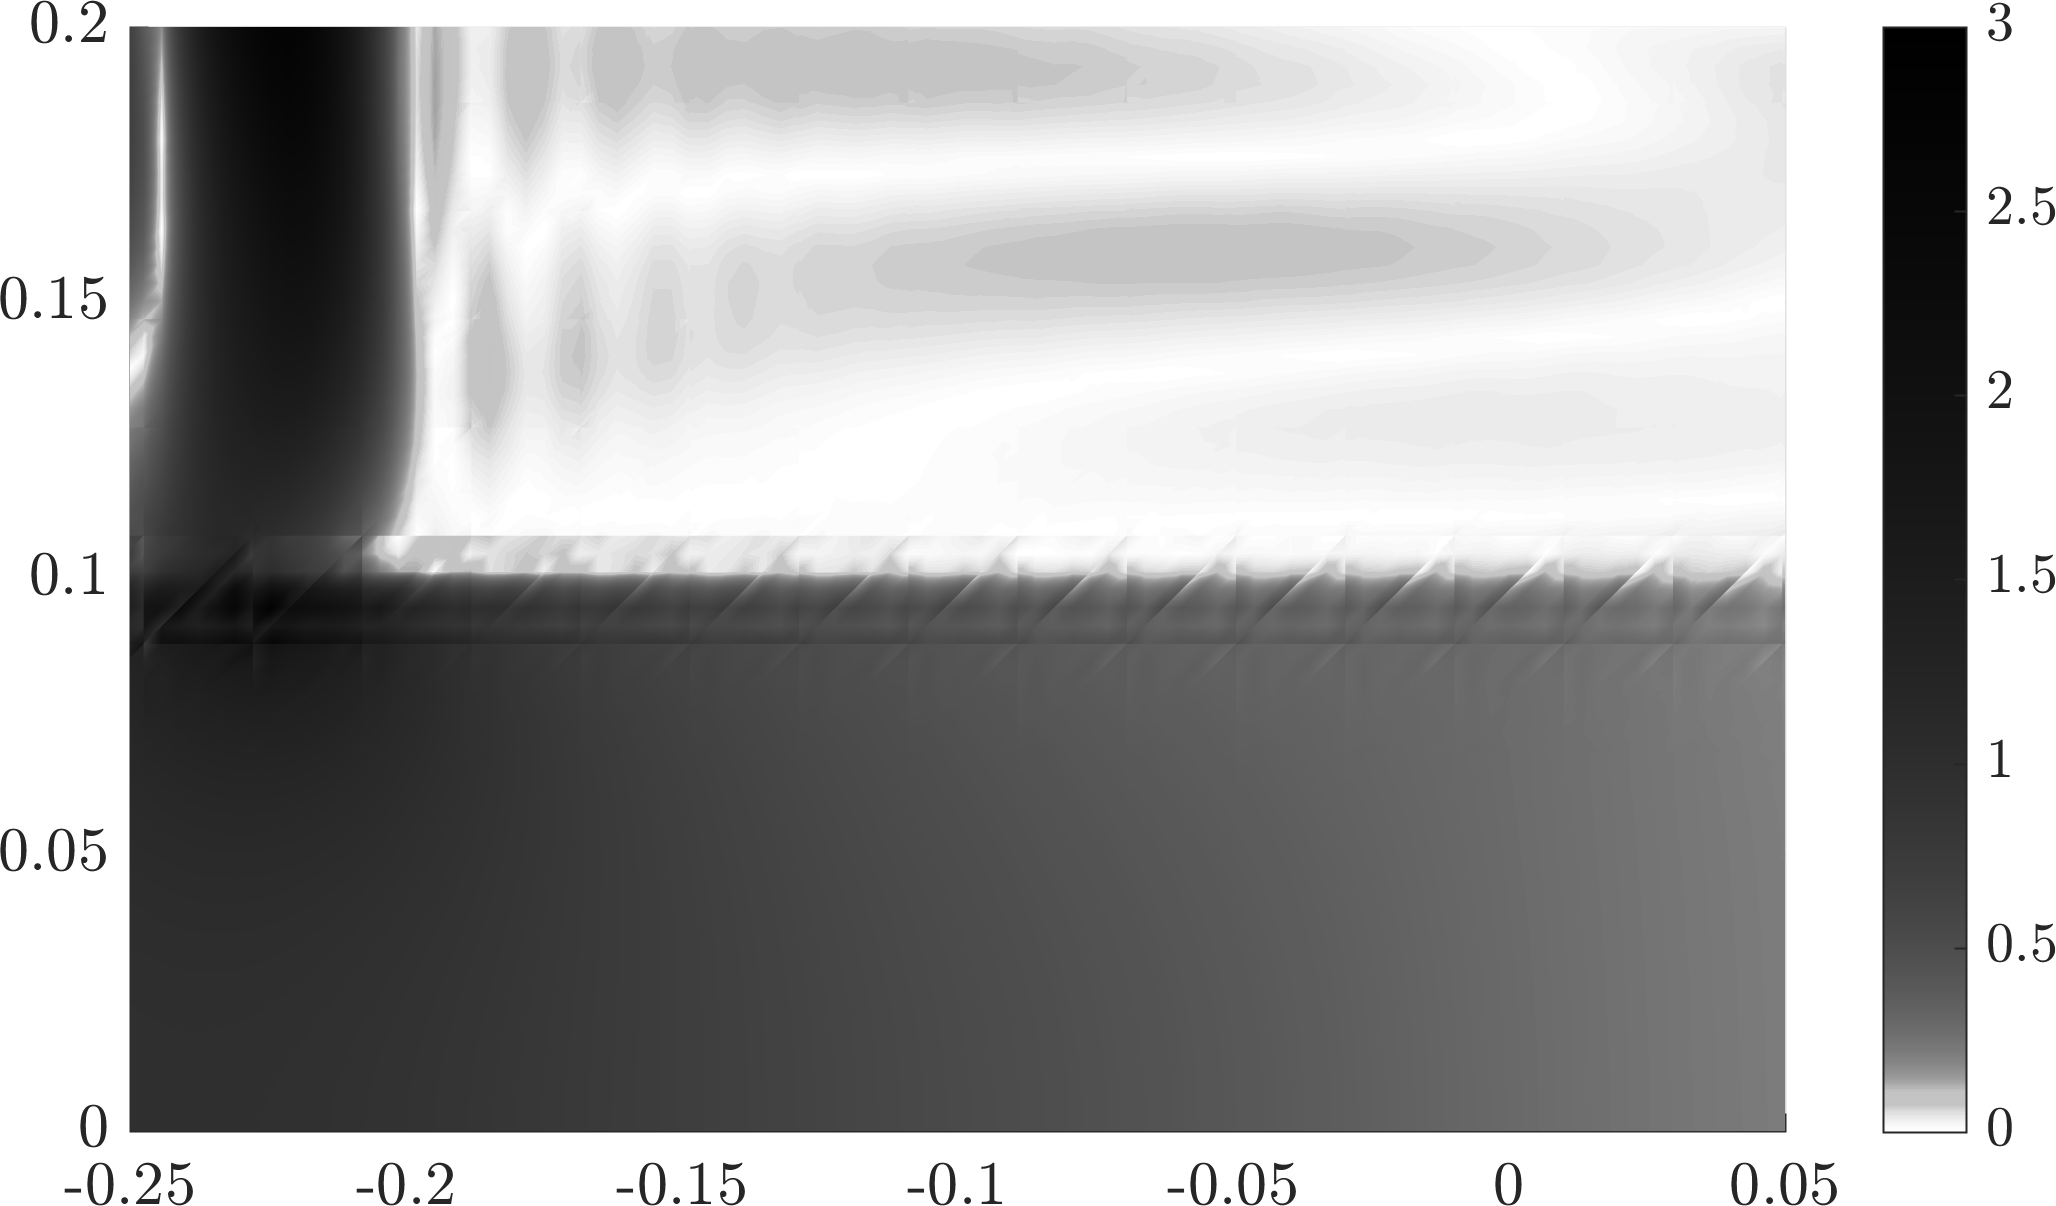
\includegraphics[height=.24\textwidth]{figs/inclusion_unaligned_zoom.png}}
\caption{Values of different solution fields at $T=.4$ for the stiff inclusion problem of Leveque \cite{leveque2002finite} with order of approximation $N=5$.}
\label{fig:incl}
\end{figure}

%We consider both aligned meshes where the inclusion boundary coincides with interior faces and an un-aligned mesh where the inclusion cuts through element interiors.  Both are constructed by dividing each element of a quadrilateral meshes along the diagonal to produce triangular meshes.  The aligned mesh is constructed using $100 \times 50$ quadrilateral elements in the $x$ and $y$ coordinates, respectively, while the un-aligned mesh was constructed using $101 \times 51$ elements.  Figure~\ref{fig:incl} shows values of $\LRb{\bm{\sigma}_{xx} + \bm{\sigma}_{yy}}$ at final time $T=.4$, along with a zoomed-in view along the interface.  The results for the interface-aligned mesh show good agreement with results in the literature \cite{leveque2002finite,kaser2006arbitrary,appelo2015energy}.  %The sub-element resolution of $\mu,\lambda$, an error is still incurred when the�mesh is un-aligned with the interface 
%For the un-aligned mesh, the sub-element resolution of material data is clearly visible, though an interface error is still incurred by the under-resolution of the interface \cite{symes2009interface}.

We construct a uniform triangular mesh by dividing each element of a quadrilateral meshes along the diagonal to produce triangular meshes, using $100 \times 50$ quadrilateral elements in the $x$ and $y$ coordinates, respectively.  Penalty parameters of $\tau_v = \tau_\sigma = 1/2$ are chosen.  Figure~\ref{fig:incl} shows values of $\LRb{\bm{\sigma}_{xx} + \bm{\sigma}_{yy}}$ at final time $T=.4$.  Following \cite{leveque2002finite}, a nonlinear color scale is used in order to distinguish small-amplitude waves.  The results show qualitatively good agreement with results in the literature \cite{leveque2002finite,kaser2006arbitrary,appelo2015energy}.  

%\note{Finish}

\subsubsection{Heterogeneous anisotropic material}

We next examine a model wave propagation problem in heterogeneous anisotropy media \cite{carcione1988wave,komatitsch2000simulation,de2007arbitrary}.   The density $\rho = 7100$ is constant over the domain, while the entries of the stiffness matrix $\bm{C}$ are taken to be
\begin{align*}
\bm{C}_{11} &= .165, \quad \bm{C}_{12} = .05, \quad \bm{C}_{22} = .062, \quad \bm{C}_{33} = .0396, \qquad x < 0\\
\bm{C}_{11} &= .165, \quad \bm{C}_{12} = .0858, \quad \bm{C}_{22} = .165, \quad \bm{C}_{33} = .0396, \qquad x > 0,
\end{align*}
with the remaining entries determined by symmetry or set to zero if unspecified.  For $ x < 0$, this corresponds to an anisotropic material, while for $x > 0$, this corresponds to an isotropic material with $\mu = .0396, \lambda = .0858$.

The computational domain is taken to be $[-.32, .32]^2$, and following \cite{komatitsch2000simulation,de2007arbitrary}, we use $N=5$ and a triangular mesh of $32768$ elements constructed by subdividing a grid of $128\times 128$ uniform quadrilaterals.  This mesh corresponds to an element size of $.005$, as used in \cite{komatitsch2000simulation,de2007arbitrary}.  Forcing is applied to the $y$-component of the velocity by a Ricker wavelet point source 
\[
f(\bm{x},t) = \LRp{1 - 2(\pi f_0 (t-t_0))^2} e^{-(\pi f_0 (t-t_0))^2}\delta(x-x_0),
\]
where $x_0 = -.02$, $f_0 = .17$, and $t_0 = 1/f_0$.\footnote{All values and units are adapted from \cite{komatitsch2000simulation,de2007arbitrary}, and correspond to units of meters, kg, and microseconds.}  The penalty parameters are taken to be $\tau_\rho = \tau_\sigma = 1/2$.  Figure~\ref{fig:aniso} shows the $y$-component of velocity $\bm{v}_2$ at times $T = 30 \mu s$ (zoomed in) and $T= 60 \mu s$.  Both results show qualitative agreement with reference results from \cite{carcione1988wave,komatitsch2000simulation,de2007arbitrary}.  
\begin{figure}
\centering
%\subfloat[$\bm{v}_1$]{\includegraphics[width=.45\textwidth]{}}
%\subfloat[$\bm{v}_2$]{\includegraphics[width=.45\textwidth]{}}
\subfloat[$T=30 \mu s$ (zoomed in)]{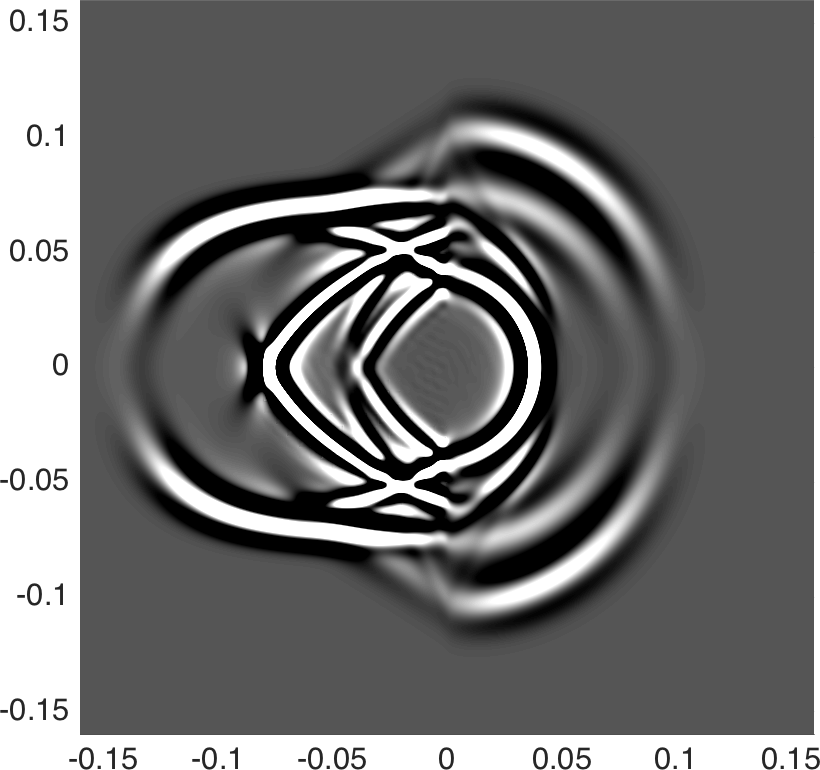
\includegraphics[height=18em]{figs/aniso1.png}}
\hspace{3em}
\subfloat[$T=60 \mu s$]{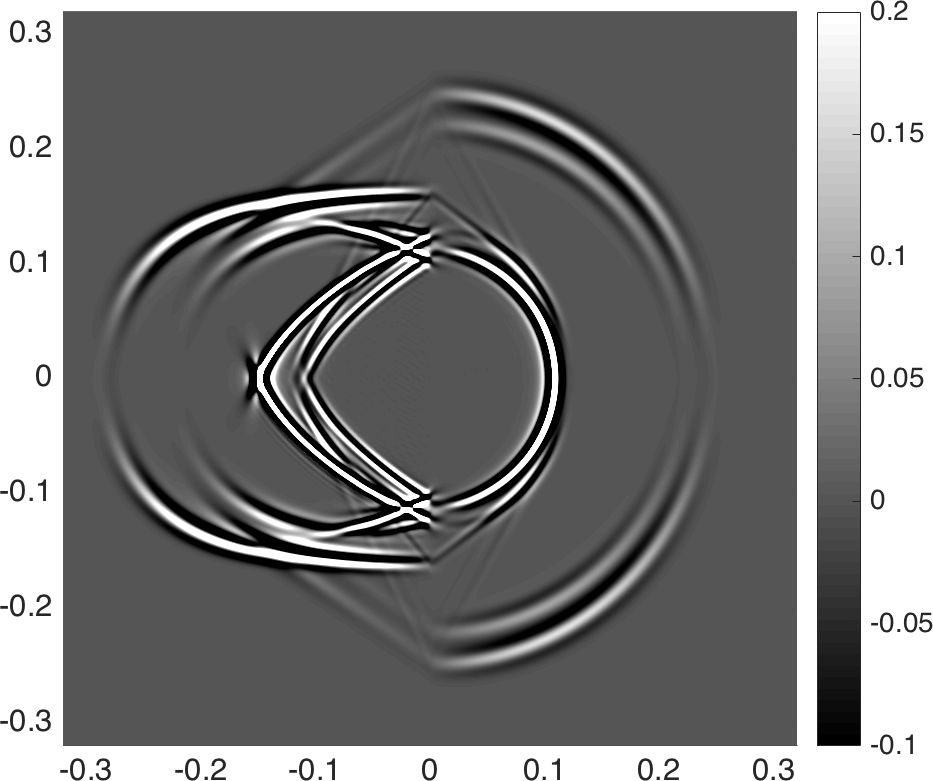
\includegraphics[height=18.25em]{figs/aniso2.png}}
\caption{An example of wave propagation in heterogeneous anisotropic media.  The vertical component of the velocity $\bm{v}_2$ is shown at $T = 30$ and $T=60$ microseconds. }
\label{fig:aniso}
\end{figure}

\subsection{A three-dimensional example}

Finally, we present a three-dimensional example of elastic wave propagation in heterogeneous media with sub-element variations and a discontinuity across an interface.  We consider isotropic elastic wave propagation on the cube $[-.5,.5]^3$ with a discontinuity in material coefficients across $z = 0$
\[
\rho = 1, \qquad \mu(\bm{x}) = \begin{cases}
2 + w(\bm{x}), & z < 0\\
1 + w(\bm{x}), & z > 0
\end{cases},
\qquad
\lambda(\bm{x}) = \begin{cases}
2, & z < 0\\
1, & z > 0
\end{cases}
\]
where $w(\bm{x})$ is a spatially varying weight.  
%isotropic media for $z < 0$ and a transversely isotropic media for $z > 0$.  For isotropic media, we take $\mu(\bm{x}) = w(\bm{x})$ and $\lambda(\bm{x}) = 2w(\bm{x})$, where $w(\bm{x})$ is a spatially varying weight function to be specified.  For $z > 0$, we take $\bm{C}$ to be 
%\[
%\bm{C} &= w(\bm{x}) \LRp{
%\begin{array}{cccccc}
%c_{11} & c_{12} & \lambda & & &\\
%c_{12} & c_{11} & \lambda & & &\\
%\lambda & \lambda & 2\mu+\lambda & & &\\
%& & & \mu & &\\
%& & & & \mu &\\
%& & & & & (c_{11}-c_{12})/2\\
%\end{array}
%}
%\]
%with $c_{11} = 1$ and $c_{12} = .5$.  
Forcing is applied to the $x$-component of velocity through a smoothed point source and Ricker wavelet
\[
f(\bm{x},t) = \LRp{1 - 2(\pi f_0 (t-t_0))^2} e^{-(\pi f_0 (t-t_0))^2}e^{- \LRp{a \nor{\bm{x}-\bm{x}_0}}^2}
\]
where $\bm{x}_0 = (0,0,.1)^T$, $a = 100$, $f_0 = 10$, and $t_0 = 1/f_0$.  
\begin{figure}
\centering
\subfloat[Computational mesh]{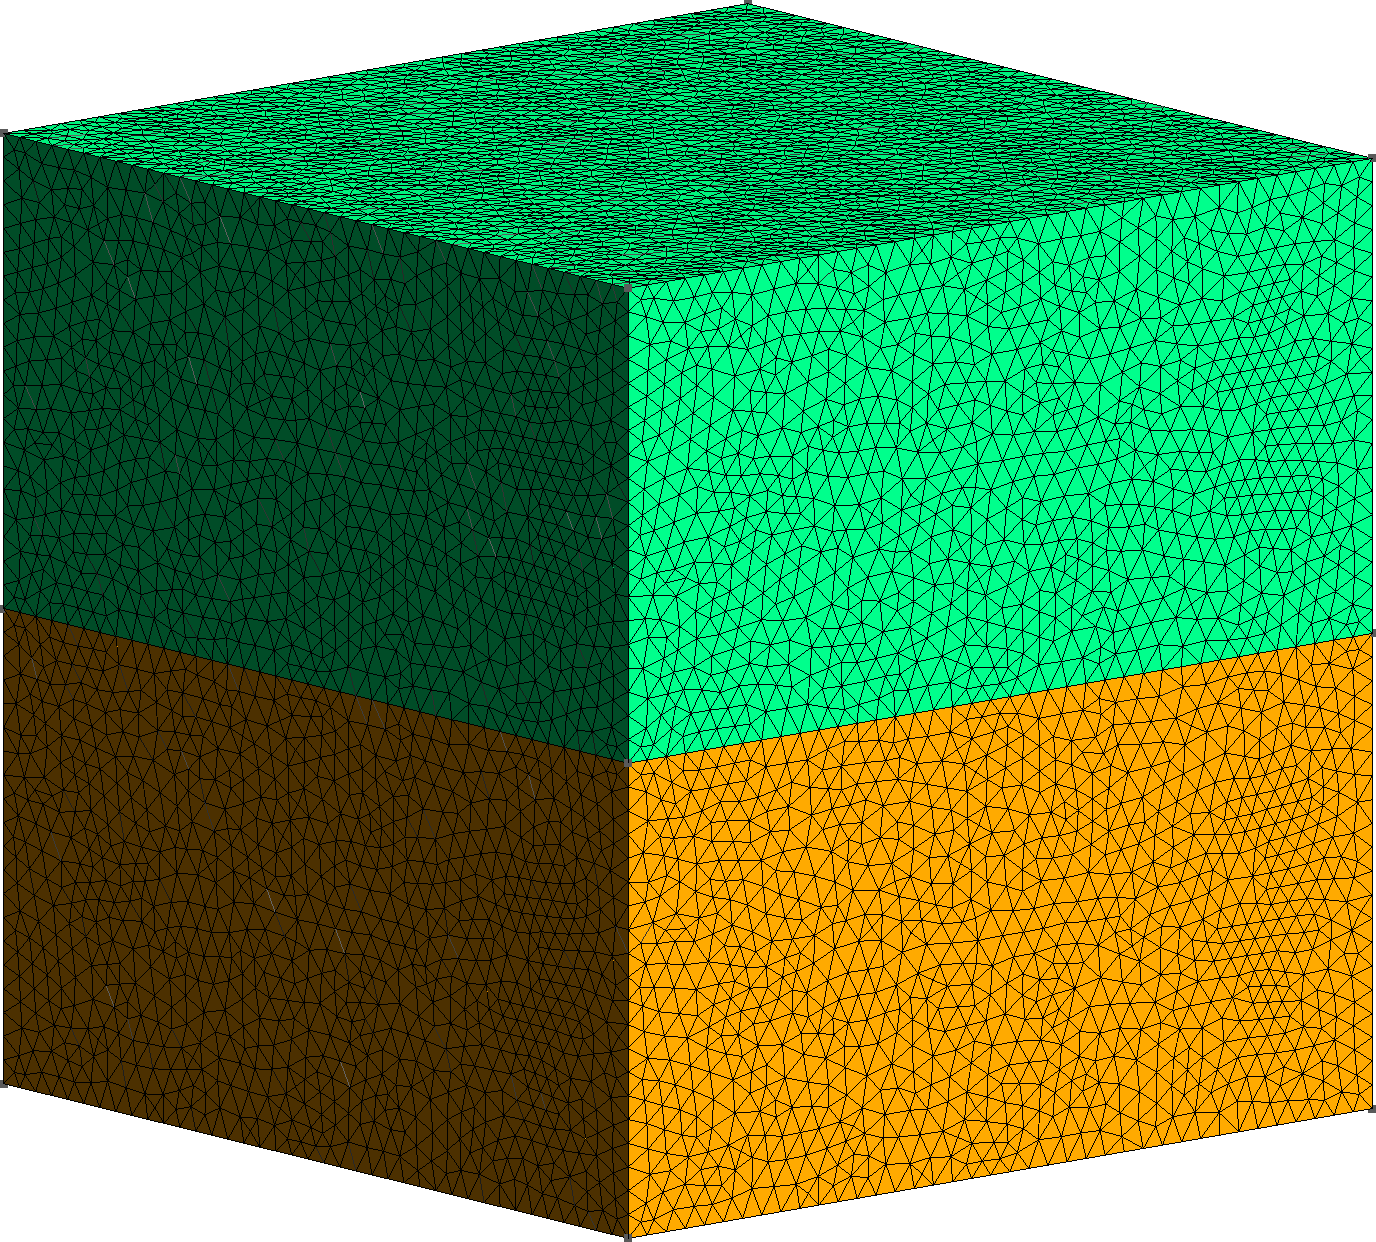
\includegraphics[width=.28\textwidth]{figs/cubeSplitFine.png}\label{subfig:mesh}}
\hspace{.5em}
\subfloat[$w(\bm{x}) = 0$]{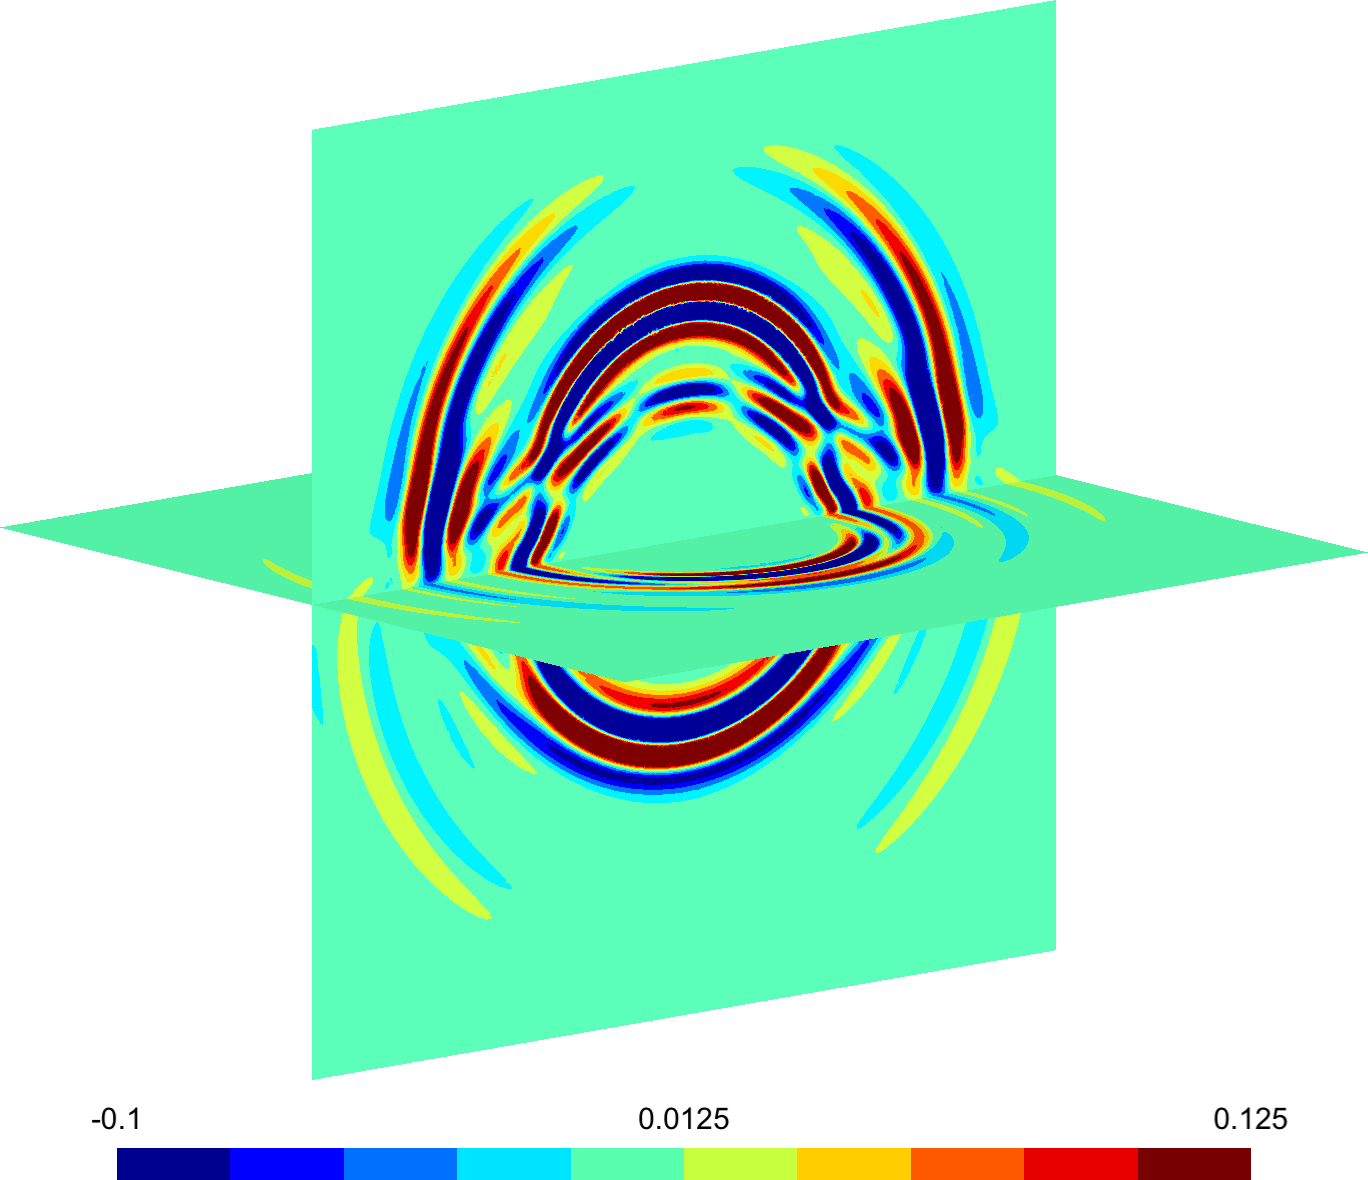
\includegraphics[width=.35\textwidth]{figs/pplane0.png}}
%\hspace{.25em}
\subfloat[$w(\bm{x})  = .5 \cos(3\pi x)\cos(3\pi y)\cos(3\pi z) $]{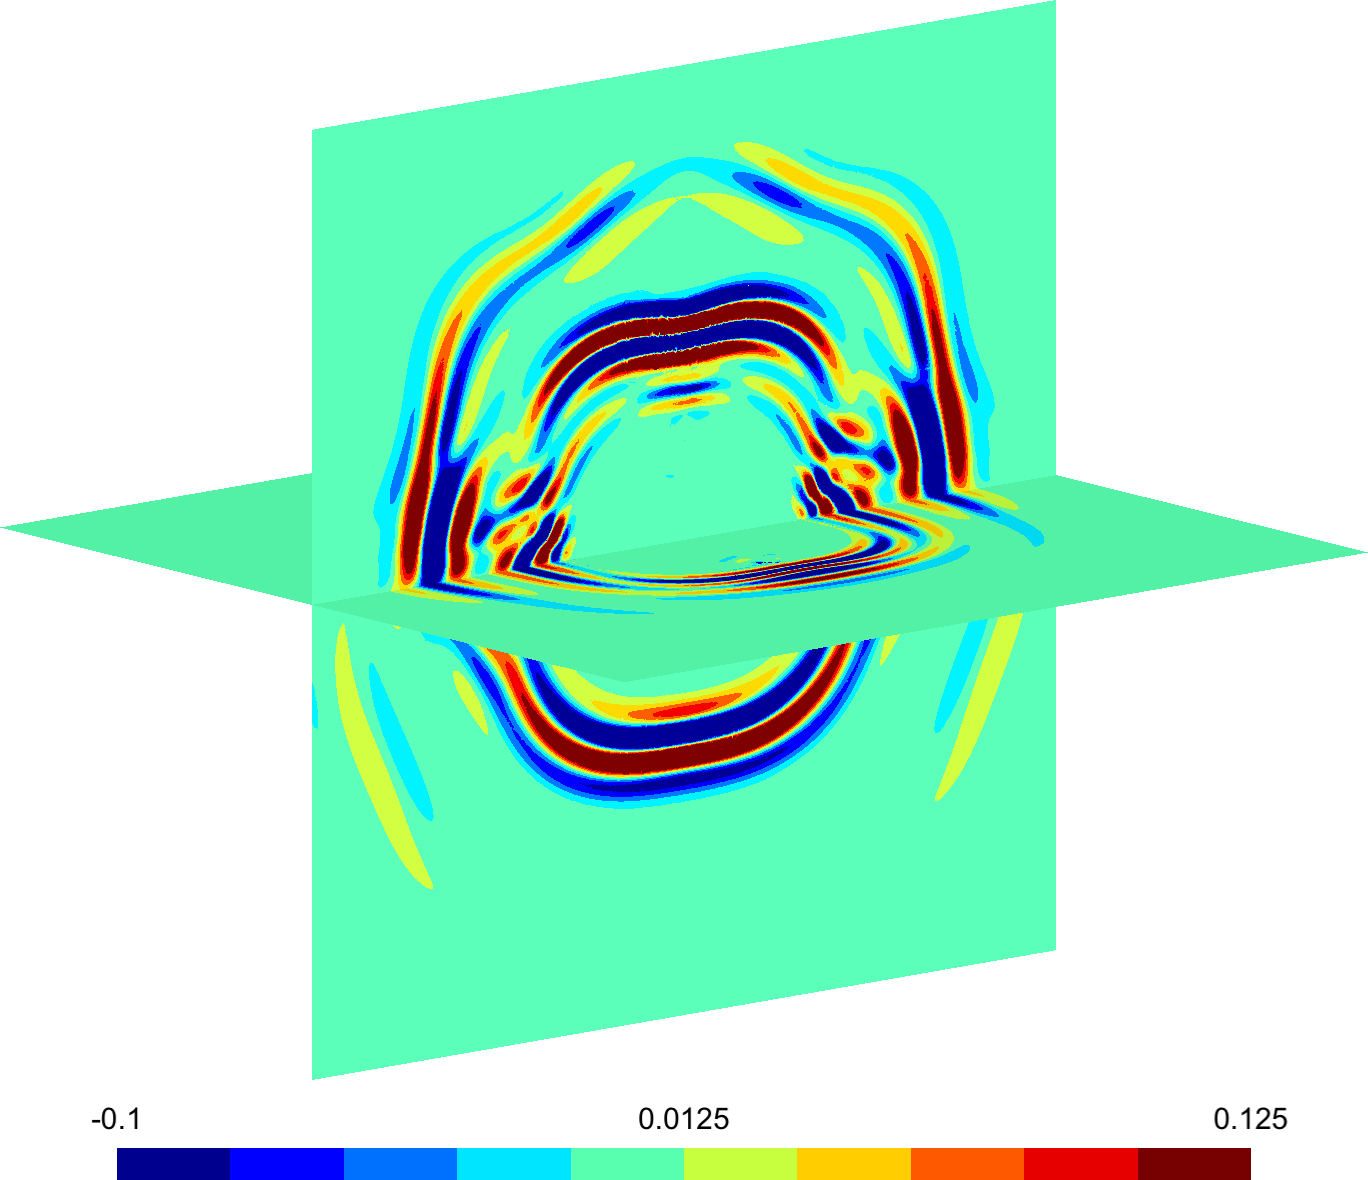
\includegraphics[width=.35\textwidth]{figs/pplanew0.png}}
\caption{Mesh and $xz$, $xy$ slices of $\bm{v}_1$ at $T = .5$.  The order of approximation is taken to be $N=5$.  }
\label{fig:3d}
\end{figure}
Figure~\ref{fig:3d} shows the $x$-velocity of the computed solution at $T = .5$ with
\[
w(\bm{x}) = .5 \cos(3\pi x)\cos(3\pi y)\cos(3\pi z), 
\]  
as well as $w(\bm{x}) = 0$ for reference.  Figure~\ref{subfig:mesh} shows the unstructured mesh of 222824 tetrahedral elements of degree $N=5$ used to compute both solutions. 

 These computations are performed on an AMD Tahiti GPU, following the implementation of GPU-accelerated DG methods outlined in \cite{klockner2009nodal}.  This approach breaks the computational work for each time-step into \emph{volume} and \emph{surface} kernels (for the evaluation of the DG formulation) and an \emph{update} kernel (for the application of a time integration method).    In this implementation, we apply the weight-adjusted mass matrix inverse within the update kernel as well.  Strategies for volume and surface kernels follow \cite{klockner2009nodal}, while computational approaches for WADG are outlined in \cite{chan2016weight2}.  

\section{Conclusions}
\label{sec:conclusions}

This work presents a weight-adjusted discontinuous Galerkin (WADG) method for the linear elastic wave equations with arbitrary heterogeneous media.  The method is energy stable and high order accurate for arbitrary stiffness matrices, and a slight modification results in an energy stable method for curvilinear meshes as well.  The penalty numerical fluxes for this formulation are simple to derive and implement, and their lack of dependence on the stiffness matrix allows for a unified treatment of isotropic and anisotropic media.  Numerical examples confirm the accuracy of this method for analytic solutions in of the elastic wave equations, as well as its high order accuracy with respect to a reference solution for smoothly varying heterogeneous media.  Results obtained using this method also show good agreement with existing results in the literature for both problems involving both isotropic and anisotropic heterogeneous media.  

We note that the implementation of this method reduces to the application of the weight-adjusted mass matrix inverse and the evaluation of constant-coefficient terms in the DG formulation.  The cost of the latter step can be reduced (especially at high orders of approximation) by using fast methods based on Bernstein-Bezier bases for the application of derivative and lift matrices for constant-coefficient terms \cite{chan2015bbdg}.  %Finally, the approach presented here is more generally applicable to problems involving a weighted mass matrix with a matrix-valued weight, including hyperbolic systems of PDEs with a left hand side of the form $\bm{A}_{0}(\bm{x})\pd{\bm{U}}{t}$, such as Maxwell's equations for cloaking problems \cite{li2012time}.  

%Extension to hybrid meshes in 3D, care must be taken with pyramids \cite{chan2015orthogonal, chan2015gpu}.

\section{Acknowledgments}

The author gratefully thanks Thomas Hagstrom, Tim Warburton, Axel Modave, Ruichao Ye, and Mario Bencomo for helpful and informative discussions.  

\bibliographystyle{unsrt}
\bibliography{dgpenalty}


\end{document}


